
%% bare_jrnl_compsoc.tex
%% V1.4a
%% 2014/09/17
%% by Michael Shell
%% See:
%% http://www.michaelshell.org/
%% for current contact information.
%%
%% This is a skeleton file demonstrating the use of IEEEtran.cls
%% (requires IEEEtran.cls version 1.8a or later) with an IEEE
%% Computer Society journal paper.
%%
%% Support sites:
%% http://www.michaelshell.org/tex/ieeetran/
%% http://www.ctan.org/tex-archive/macros/latex/contrib/IEEEtran/
%% and
%% http://www.ieee.org/

%%*************************************************************************
%% Legal Notice:
%% This code is offered as-is without any warranty either expressed or
%% implied; without even the implied warranty of MERCHANTABILITY or
%% FITNESS FOR A PARTICULAR PURPOSE!
%% User assumes all risk.
%% In no event shall IEEE or any contributor to this code be liable for
%% any damages or losses, including, but not limited to, incidental,
%% consequential, or any other damages, resulting from the use or misuse
%% of any information contained here.
%%
%% All comments are the opinions of their respective authors and are not
%% necessarily endorsed by the IEEE.
%%
%% This work is distributed under the LaTeX Project Public License (LPPL)
%% ( http://www.latex-project.org/ ) version 1.3, and may be freely used,
%% distributed and modified. A copy of the LPPL, version 1.3, is included
%% in the base LaTeX documentation of all distributions of LaTeX released
%% 2003/12/01 or later.
%% Retain all contribution notices and credits.
%% ** Modified files should be clearly indicated as such, including  **
%% ** renaming them and changing author support contact information. **
%%
%% File list of work: IEEEtran.cls, IEEEtran_HOWTO.pdf, bare_adv.tex,
%%                    bare_conf.tex, bare_jrnl.tex, bare_conf_compsoc.tex,
%%                    bare_jrnl_compsoc.tex, bare_jrnl_transmag.tex
%%*************************************************************************


% *** Authors should verify (and, if needed, correct) their LaTeX system  ***
% *** with the testflow diagnostic prior to trusting their LaTeX platform ***
% *** with production work. IEEE's font choices and paper sizes can       ***
% *** trigger bugs that do not appear when using other class files.       ***                          ***
% The testflow support page is at:
% http://www.michaelshell.org/tex/testflow/


\documentclass[10pt,journal,compsoc]{IEEEtran}
%
% If IEEEtran.cls has not been installed into the LaTeX system files,
% manually specify the path to it like:
% \documentclass[10pt,journal,compsoc]{../sty/IEEEtran}





% Some very useful LaTeX packages include:
% (uncomment the ones you want to load)


% *** MISC UTILITY PACKAGES ***
%
%\usepackage{ifpdf}
% Heiko Oberdiek's ifpdf.sty is very useful if you need conditional
% compilation based on whether the output is pdf or dvi.
% usage:
% \ifpdf
%   % pdf code
% \else
%   % dvi code
% \fi
% The latest version of ifpdf.sty can be obtained from:
% http://www.ctan.org/tex-archive/macros/latex/contrib/oberdiek/
% Also, note that IEEEtran.cls V1.7 and later provides a builtin
% \ifCLASSINFOpdf conditional that works the same way.
% When switching from latex to pdflatex and vice-versa, the compiler may
% have to be run twice to clear warning/error messages.






% *** CITATION PACKAGES ***
%
\ifCLASSOPTIONcompsoc
  % IEEE Computer Society needs nocompress option
  % requires cite.sty v4.0 or later (November 2003)
  \usepackage[nocompress]{cite}
\else
  % normal IEEE
  \usepackage{cite}
\fi
% cite.sty was written by Donald Arseneau
% V1.6 and later of IEEEtran pre-defines the format of the cite.sty package
% \cite{} output to follow that of IEEE. Loading the cite package will
% result in citation numbers being automatically sorted and properly
% "compressed/ranged". e.g., [1], [9], [2], [7], [5], [6] without using
% cite.sty will become [1], [2], [5]--[7], [9] using cite.sty. cite.sty's
% \cite will automatically add leading space, if needed. Use cite.sty's
% noadjust option (cite.sty V3.8 and later) if you want to turn this off
% such as if a citation ever needs to be enclosed in parenthesis.
% cite.sty is already installed on most LaTeX systems. Be sure and use
% version 5.0 (2009-03-20) and later if using hyperref.sty.
% The latest version can be obtained at:
% http://www.ctan.org/tex-archive/macros/latex/contrib/cite/
% The documentation is contained in the cite.sty file itself.
%
% Note that some packages require special options to format as the Computer
% Society requires. In particular, Computer Society  papers do not use
% compressed citation ranges as is done in typical IEEE papers
% (e.g., [1]-[4]). Instead, they list every citation separately in order
% (e.g., [1], [2], [3], [4]). To get the latter we need to load the cite
% package with the nocompress option which is supported by cite.sty v4.0
% and later. Note also the use of a CLASSOPTION conditional provided by
% IEEEtran.cls V1.7 and later.





% *** GRAPHICS RELATED PACKAGES ***
%
\ifCLASSINFOpdf
  % \usepackage[pdftex]{graphicx}
  % declare the path(s) where your graphic files are
  % \graphicspath{{../pdf/}{../jpeg/}}
  % and their extensions so you won't have to specify these with
  % every instance of \includegraphics
  % \DeclareGraphicsExtensions{.pdf,.jpeg,.png}
\else
  % or other class option (dvipsone, dvipdf, if not using dvips). graphicx
  % will default to the driver specified in the system graphics.cfg if no
  % driver is specified.
  % \usepackage[dvips]{graphicx}
  % declare the path(s) where your graphic files are
  % \graphicspath{{../eps/}}
  % and their extensions so you won't have to specify these with
  % every instance of \includegraphics
  % \DeclareGraphicsExtensions{.eps}
\fi
% graphicx was written by David Carlisle and Sebastian Rahtz. It is
% required if you want graphics, photos, etc. graphicx.sty is already
% installed on most LaTeX systems. The latest version and documentation
% can be obtained at:
% http://www.ctan.org/tex-archive/macros/latex/required/graphics/
% Another good source of documentation is "Using Imported Graphics in
% LaTeX2e" by Keith Reckdahl which can be found at:
% http://www.ctan.org/tex-archive/info/epslatex/
%
% latex, and pdflatex in dvi mode, support graphics in encapsulated
% postscript (.eps) format. pdflatex in pdf mode supports graphics
% in .pdf, .jpeg, .png and .mps (metapost) formats. Users should ensure
% that all non-photo figures use a vector format (.eps, .pdf, .mps) and
% not a bitmapped formats (.jpeg, .png). IEEE frowns on bitmapped formats
% which can result in "jaggedy"/blurry rendering of lines and letters as
% well as large increases in file sizes.
%
% You can find documentation about the pdfTeX application at:
% http://www.tug.org/applications/pdftex






% *** MATH PACKAGES ***
%
%\usepackage[cmex10]{amsmath}
% A popular package from the American Mathematical Society that provides
% many useful and powerful commands for dealing with mathematics. If using
% it, be sure to load this package with the cmex10 option to ensure that
% only type 1 fonts will utilized at all point sizes. Without this option,
% it is possible that some math symbols, particularly those within
% footnotes, will be rendered in bitmap form which will result in a
% document that can not be IEEE Xplore compliant!
%
% Also, note that the amsmath package sets \interdisplaylinepenalty to 10000
% thus preventing page breaks from occurring within multiline equations. Use:
%\interdisplaylinepenalty=2500
% after loading amsmath to restore such page breaks as IEEEtran.cls normally
% does. amsmath.sty is already installed on most LaTeX systems. The latest
% version and documentation can be obtained at:
% http://www.ctan.org/tex-archive/macros/latex/required/amslatex/math/





% *** SPECIALIZED LIST PACKAGES ***
%
%\usepackage{algorithmic}
% algorithmic.sty was written by Peter Williams and Rogerio Brito.
% This package provides an algorithmic environment fo describing algorithms.
% You can use the algorithmic environment in-text or within a figure
% environment to provide for a floating algorithm. Do NOT use the algorithm
% floating environment provided by algorithm.sty (by the same authors) or
% algorithm2e.sty (by Christophe Fiorio) as IEEE does not use dedicated
% algorithm float types and packages that provide these will not provide
% correct IEEE style captions. The latest version and documentation of
% algorithmic.sty can be obtained at:
% http://www.ctan.org/tex-archive/macros/latex/contrib/algorithms/
% There is also a support site at:
% http://algorithms.berlios.de/index.html
% Also of interest may be the (relatively newer and more customizable)
% algorithmicx.sty package by Szasz Janos:
% http://www.ctan.org/tex-archive/macros/latex/contrib/algorithmicx/




% *** ALIGNMENT PACKAGES ***
%
%\usepackage{array}
% Frank Mittelbach's and David Carlisle's array.sty patches and improves
% the standard LaTeX2e array and tabular environments to provide better
% appearance and additional user controls. As the default LaTeX2e table
% generation code is lacking to the point of almost being broken with
% respect to the quality of the end results, all users are strongly
% advised to use an enhanced (at the very least that provided by array.sty)
% set of table tools. array.sty is already installed on most systems. The
% latest version and documentation can be obtained at:
% http://www.ctan.org/tex-archive/macros/latex/required/tools/


% IEEEtran contains the IEEEeqnarray family of commands that can be used to
% generate multiline equations as well as matrices, tables, etc., of high
% quality.




% *** SUBFIGURE PACKAGES ***
%\ifCLASSOPTIONcompsoc
%  \usepackage[caption=false,font=footnotesize,labelfont=sf,textfont=sf]{subfig}
%\else
%  \usepackage[caption=false,font=footnotesize]{subfig}
%\fi
% subfig.sty, written by Steven Douglas Cochran, is the modern replacement
% for subfigure.sty, the latter of which is no longer maintained and is
% incompatible with some LaTeX packages including fixltx2e. However,
% subfig.sty requires and automatically loads Axel Sommerfeldt's caption.sty
% which will override IEEEtran.cls' handling of captions and this will result
% in non-IEEE style figure/table captions. To prevent this problem, be sure
% and invoke subfig.sty's "caption=false" package option (available since
% subfig.sty version 1.3, 2005/06/28) as this is will preserve IEEEtran.cls
% handling of captions.
% Note that the Computer Society format requires a sans serif font rather
% than the serif font used in traditional IEEE formatting and thus the need
% to invoke different subfig.sty package options depending on whether
% compsoc mode has been enabled.
%
% The latest version and documentation of subfig.sty can be obtained at:
% http://www.ctan.org/tex-archive/macros/latex/contrib/subfig/




% *** FLOAT PACKAGES ***
%
%\usepackage{fixltx2e}
% fixltx2e, the successor to the earlier fix2col.sty, was written by
% Frank Mittelbach and David Carlisle. This package corrects a few problems
% in the LaTeX2e kernel, the most notable of which is that in current
% LaTeX2e releases, the ordering of single and double column floats is not
% guaranteed to be preserved. Thus, an unpatched LaTeX2e can allow a
% single column figure to be placed prior to an earlier double column
% figure. The latest version and documentation can be found at:
% http://www.ctan.org/tex-archive/macros/latex/base/


%\usepackage{stfloats}
% stfloats.sty was written by Sigitas Tolusis. This package gives LaTeX2e
% the ability to do double column floats at the bottom of the page as well
% as the top. (e.g., "\begin{figure*}[!b]" is not normally possible in
% LaTeX2e). It also provides a command:
%\fnbelowfloat
% to enable the placement of footnotes below bottom floats (the standard
% LaTeX2e kernel puts them above bottom floats). This is an invasive package
% which rewrites many portions of the LaTeX2e float routines. It may not work
% with other packages that modify the LaTeX2e float routines. The latest
% version and documentation can be obtained at:
% http://www.ctan.org/tex-archive/macros/latex/contrib/sttools/
% Do not use the stfloats baselinefloat ability as IEEE does not allow
% \baselineskip to stretch. Authors submitting work to the IEEE should note
% that IEEE rarely uses double column equations and that authors should try
% to avoid such use. Do not be tempted to use the cuted.sty or midfloat.sty
% packages (also by Sigitas Tolusis) as IEEE does not format its papers in
% such ways.
% Do not attempt to use stfloats with fixltx2e as they are incompatible.
% Instead, use Morten Hogholm'a dblfloatfix which combines the features
% of both fixltx2e and stfloats:
%
% \usepackage{dblfloatfix}
% The latest version can be found at:
% http://www.ctan.org/tex-archive/macros/latex/contrib/dblfloatfix/




%\ifCLASSOPTIONcaptionsoff
%  \usepackage[nomarkers]{endfloat}
% \let\MYoriglatexcaption\caption
% \renewcommand{\caption}[2][\relax]{\MYoriglatexcaption[#2]{#2}}
%\fi
% endfloat.sty was written by James Darrell McCauley, Jeff Goldberg and
% Axel Sommerfeldt. This package may be useful when used in conjunction with
% IEEEtran.cls'  captionsoff option. Some IEEE journals/societies require that
% submissions have lists of figures/tables at the end of the paper and that
% figures/tables without any captions are placed on a page by themselves at
% the end of the document. If needed, the draftcls IEEEtran class option or
% \CLASSINPUTbaselinestretch interface can be used to increase the line
% spacing as well. Be sure and use the nomarkers option of endfloat to
% prevent endfloat from "marking" where the figures would have been placed
% in the text. The two hack lines of code above are a slight modification of
% that suggested by in the endfloat docs (section 8.4.1) to ensure that
% the full captions always appear in the list of figures/tables - even if
% the user used the short optional argument of \caption[]{}.
% IEEE papers do not typically make use of \caption[]'s optional argument,
% so this should not be an issue. A similar trick can be used to disable
% captions of packages such as subfig.sty that lack options to turn off
% the subcaptions:
% For subfig.sty:
% \let\MYorigsubfloat\subfloat
% \renewcommand{\subfloat}[2][\relax]{\MYorigsubfloat[]{#2}}
% However, the above trick will not work if both optional arguments of
% the \subfloat command are used. Furthermore, there needs to be a
% description of each subfigure *somewhere* and endfloat does not add
% subfigure captions to its list of figures. Thus, the best approach is to
% avoid the use of subfigure captions (many IEEE journals avoid them anyway)
% and instead reference/explain all the subfigures within the main caption.
% The latest version of endfloat.sty and its documentation can obtained at:
% http://www.ctan.org/tex-archive/macros/latex/contrib/endfloat/
%
% The IEEEtran \ifCLASSOPTIONcaptionsoff conditional can also be used
% later in the document, say, to conditionally put the References on a
% page by themselves.




% *** PDF, URL AND HYPERLINK PACKAGES ***
%
%\usepackage{url}
% url.sty was written by Donald Arseneau. It provides better support for
% handling and breaking URLs. url.sty is already installed on most LaTeX
% systems. The latest version and documentation can be obtained at:
% http://www.ctan.org/tex-archive/macros/latex/contrib/url/
% Basically, \url{my_url_here}.





% *** Do not adjust lengths that control margins, column widths, etc. ***
% *** Do not use packages that alter fonts (such as pslatex).         ***
% There should be no need to do such things with IEEEtran.cls V1.6 and later.
% (Unless specifically asked to do so by the journal or conference you plan
% to submit to, of course. )


% correct bad hyphenation here
\hyphenation{op-tical net-works semi-conduc-tor}

\usepackage[normalem]{ulem}
\usepackage{algpseudocode}
\usepackage{algorithm}

\usepackage{algorithm,algpseudocode}
\makeatletter
\newcommand{\StatexIndent}[1][3]{%
  \setlength\@tempdima{\algorithmicindent}%
  \Statex\hskip\dimexpr#1\@tempdima\relax}
\algdef{S}[WHILE]{WhileNoDo}[1]{\algorithmicwhile\ #1}%
\makeatother


\usepackage{amsmath}
%\usepackage{url}
\usepackage{graphicx}
\usepackage{subfigure}
\usepackage{multirow}
 \usepackage{url}
\usepackage[table]{xcolor}

\usepackage{footnote}
\makesavenoteenv{tabular}
\makesavenoteenv{table}

\algrenewcommand{\algorithmicrequire}{\textbf{Input:}}
\algrenewcommand{\algorithmicensure}{\textbf{Output:}}
\renewcommand{\algorithmicforall}{\textbf{for each}}

\begin{document}
\bstctlcite{IEEEexample:BSTcontrol}
%
% paper title
% Titles are generally capitalized except for words such as a, an, and, as,
% at, but, by, for, in, nor, of, on, or, the, to and up, which are usually
% not capitalized unless they are the first or last word of the title.
% Linebreaks \\ can be used within to get better formatting as desired.
% Do not put math or special symbols in the title.
\title{An interleaving approach to combinatorial testing and failure-inducing interaction identification}
%
%
% author names and IEEE memberships
% note positions of commas and nonbreaking spaces ( ~ ) LaTeX will not break
% a structure at a ~ so this keeps an author's name from being broken across
% two lines.
% use \thanks{} to gain access to the first footnote area
% a separate \thanks must be used for each paragraph as LaTeX2e's \thanks
% was not built to handle multiple paragraphs
%
%
%\IEEEcompsocitemizethanks is a special \thanks that produces the bulleted
% lists the Computer Society journals use for "first footnote" author
% affiliations. Use \IEEEcompsocthanksitem which works much like \item
% for each affiliation group. When not in compsoc mode,
% \IEEEcompsocitemizethanks becomes like \thanks and
% \IEEEcompsocthanksitem becomes a line break with idention. This
% facilitates dual compilation, although admittedly the differences in the
% desired content of \author between the different types of papers makes a
% one-size-fits-all approach a daunting prospect. For instance, compsoc
% journal papers have the author affiliations above the "Manuscript
% received ..."  text while in non-compsoc journals this is reversed. Sigh.
\author{ Xintao Niu, Changhai Nie,~\IEEEmembership{Member,~IEEE,} Hareton Leung,~\IEEEmembership{Member,~IEEE,}
   Jeff Y. Lei,~\IEEEmembership{Member,~IEEE,}
   Xiaoyin Wang, ~\IEEEmembership{Member,~IEEE,}
   JiaXi Xu and Yan Wang

%\author{Michael~Shell,~\IEEEmembership{Member,~IEEE,}
%        John~Doe,~\IEEEmembership{Fellow,~OSA,}
%        and~Jane~Doe,~\IEEEmembership{Life~Fellow,~IEEE}% <-this % stops a space
\IEEEcompsocitemizethanks{\IEEEcompsocthanksitem Xintao Niu and Changhai Nie are with the State Key Laboratory for Novel Software Technology, Nanjing University, China, 210023. \protect\\
% note need leading \protect in front of \\ to get a newline within \thanks as
% \\ is fragile and will error, could use \hfil\break instead.
E-mail: niuxintao@gmail.com, changhainie@nju.edu.cn
% note need leading \protect in front of \\ to get a newline within \thanks as
% \\ is fragile and will error, could use \hfil\break instead.
\IEEEcompsocthanksitem Hareton Leung is with Department of computing, Hong Kong Polytechnic University, Kowloon, Hong Kong. \protect\\
  E-mail: hareton.leung@polyu.edu.hk
\IEEEcompsocthanksitem Jeff Y. Lei is with Department of Computer Science and Engineering, The University of Texas at Arlington, Arlington, Texas. \protect\\
  E-mail: ylei@cse.uta.edu
\IEEEcompsocthanksitem Xiaoyin Wang is with Department of Computer Science, University of Texas at San Antonio. \protect\\
  E-mail: Xiaoyin.Wang@utsa.edu
\IEEEcompsocthanksitem JiaXi Xu and Yan Wang are with School of Information Engineering, Nanjing Xiaozhuang University. \protect\\
  E-mail: xujiaxi@njxzc.edu.cn, wangyan@njxzc.edu.cn}% <-this % stops an unwanted space
\thanks{Manuscript received April 19, 2005; revised September 17, 2014.}}

%\IEEEcompsocitemizethanks{



% note the % following the last \IEEEmembership and also \thanks -
% these prevent an unwanted space from occurring between the last author name
% and the end of the author line. i.e., if you had this:
%
% \author{....lastname \thanks{...} \thanks{...} }
%                     ^------------^------------^----Do not want these spaces!
%
% a space would be appended to the last name and could cause every name on that
% line to be shifted left slightly. This is one of those "LaTeX things". For
% instance, "\textbf{A} \textbf{B}" will typeset as "A B" not "AB". To get
% "AB" then you have to do: "\textbf{A}\textbf{B}"
% \thanks is no different in this regard, so shield the last } of each \thanks
% that ends a line with a % and do not let a space in before the next \thanks.
% Spaces after \IEEEmembership other than the last one are OK (and needed) as
% you are supposed to have spaces between the names. For what it is worth,
% this is a minor point as most people would not even notice if the said evil
% space somehow managed to creep in.



% The paper headers
\markboth{Journal of \LaTeX\ Class Files,~Vol.~13, No.~9, September~2014}%
{Shell \MakeLowercase{\textit{et al.}}: Bare Demo of IEEEtran.cls for Computer Society Journals}
% The only time the second header will appear is for the odd numbered pages
% after the title page when using the twoside option.
%
% *** Note that you probably will NOT want to include the author's ***
% *** name in the headers of peer review papers.                   ***
% You can use \ifCLASSOPTIONpeerreview for conditional compilation here if
% you desire.



% The publisher's ID mark at the bottom of the page is less important with
% Computer Society journal papers as those publications place the marks
% outside of the main text columns and, therefore, unlike regular IEEE
% journals, the available text space is not reduced by their presence.
% If you want to put a publisher's ID mark on the page you can do it like
% this:
%\IEEEpubid{0000--0000/00\$00.00~\copyright~2014 IEEE}
% or like this to get the Computer Society new two part style.
%\IEEEpubid{\makebox[\columnwidth]{\hfill 0000--0000/00/\$00.00~\copyright~2014 IEEE}%
%\hspace{\columnsep}\makebox[\columnwidth]{Published by the IEEE Computer Society\hfill}}
% Remember, if you use this you must call \IEEEpubidadjcol in the second
% column for its text to clear the IEEEpubid mark (Computer Society jorunal
% papers don't need this extra clearance.)



% use for special paper notices
%\IEEEspecialpapernotice{(Invited Paper)}



% for Computer Society papers, we must declare the abstract and index terms
% PRIOR to the title within the \IEEEtitleabstractindextext IEEEtran
% command as these need to go into the title area created by \maketitle.
% As a general rule, do not put math, special symbols or citations
% in the abstract or keywords.
\IEEEtitleabstractindextext{%
\begin{abstract}
Combinatorial testing(CT) seeks to detect potential faults caused by various interactions of factors that can influence the software systems. When applying CT, it is a common practice to first generate a set of test cases to cover each possible interaction and then to identify the failure-inducing interaction after a failure is detected. Although this conventional procedure is simple and forthright, we conjecture that it is not the ideal choice in practice. This is because 1) testers desire to identify the root cause of failures before all the needed test cases are generated and executed 2) the early identified failure-inducing interactions can guide the remaining test case generation so that many unnecessary and invalid test cases can be avoided. For these reasons, we propose a novel CT framework that allows both generation and identification process to interact with each other. As a result, both generation and identification stages will be done more effectively and efficiently. We conducted a series of empirical studies on several open-source software, the results of which show that our framework can identify the failure-inducing interactions more quickly than traditional approaches while requiring fewer test cases.
\end{abstract}

% Note that keywords are not normally used for peerreview papers.
\begin{IEEEkeywords}
Software Testing, Combinatorial Testing, Covering Array, Failure-inducing interactions
\end{IEEEkeywords}}


% make the title area
 \maketitle


% To allow for easy dual compilation without having to reenter the
% abstract/keywords data, the \IEEEtitleabstractindextext text will
% not be used in maketitle, but will appear (i.e., to be "transported")
% here as \IEEEdisplaynontitleabstractindextext when the compsoc
% or transmag modes are not selected <OR> if conference mode is selected
% - because all conference papers position the abstract like regular
% papers do.
\IEEEdisplaynontitleabstractindextext
% \IEEEdisplaynontitleabstractindextext has no effect when using
% compsoc or transmag under a non-conference mode.



% For peer review papers, you can put extra information on the cover
% page as needed:
% \ifCLASSOPTIONpeerreview
% \begin{center} \bfseries EDICS Category: 3-BBND \end{center}
% \fi
%
% For peerreview papers, this IEEEtran command inserts a page break and
% creates the second title. It will be ignored for other modes.
\IEEEpeerreviewmaketitle



\IEEEraisesectionheading{\section{Introduction}\label{sec:introduction}}
% Computer Society journal (but not conference!) papers do something unusual
% with the very first section heading (almost always called "Introduction").
% They place it ABOVE the main text! IEEEtran.cls does not automatically do
% this for you, but you can achieve this effect with the provided
% \IEEEraisesectionheading{} command. Note the need to keep any \label that
% is to refer to the section immediately after \section in the above as
% \IEEEraisesectionheading puts \section within a raised box.




% The very first letter is a 2 line initial drop letter followed
% by the rest of the first word in caps (small caps for compsoc).
%
% form to use if the first word consists of a single letter:
% \IEEEPARstart{A}{demo} file is ....
%
% form to use if you need the single drop letter followed by
% normal text (unknown if ever used by IEEE):
% \IEEEPARstart{A}{}demo file is ....
%
% Some journals put the first two words in caps:
% \IEEEPARstart{T}{his demo} file is ....
%
% Here we have the typical use of a "T" for an initial drop letter
% and "HIS" in caps to complete the first word.
\IEEEPARstart{M}odern software is becoming more and more complex. To test such software is challenging, as the candidate factors that can influence the system's behaviour, e.g., configuration options, system inputs, message events, are enormous. Even worse, the interactions between these factors can also crash the system, e.g., the incompatibility problems. In consideration of the scale of the industrial software, to test all the possible interactions of all the factors (we call them the interaction space) is not feasible, and even if it is possible, it is resource-inefficient to test all the interactions.

Many empirical studies show that, in real software systems, the effective interaction space, i.e., targeting fault detection, makes up only a small proportion of the overall interaction space \cite{kuhn2002investigation,kuhn2004software}. Further, the number of factors involved in these effective interactions is relatively small, of which 4 to 6 is usually the upper bounds\cite{kuhn2002investigation}. With this observation, applying Combinatorial testing(CT) in practice is appealing, as it is proven to be effective to detect the interaction faults in the system.

CT tests software with an elaborate test suite which checks all the required parameter value combinations. A typical CT life-cycle is shown in Figure \ref{ct-life}, which contains four main testing stages. At the very beginning of the testing, engineers should extract the specific model of the software under test (SUT). In detail, they should identify the factors, such as user inputs, and configure options, that could affect the system's behavior. Further effort is required to figure out the constraints and dependencies among each factor and corresponding values for valid testing. After the modeling stage, a set of test cases should be generated and executed to expose the potential faults in the system. In CT, each test case is a set of assignments of all the factors in the test model. Thus, when such a test case is executed, all the interactions contained in the test case are deemed to be checked. The main target of this stage is to design a relatively small set of test cases to achieve some specific coverage. The third testing stage in this cycle is the fault localization, which is responsible for identifying the failure-inducing interactions. To characterize the failure-inducing interactions of corresponding factors and values is important for future bug fixing, as it will reduce the scope of suspicious code to be inspected. The last testing stage of CT is evaluation. In this stage, testers will assess the quality of the previously conducted testing tasks. If the assessment result shows that the previous testing process does not fulfill the testing requirement, some testing stages should be improved, and sometimes, may even need to be re-conducted.

%based on metrics such as whether the failure-inducing interactions can reflect the failures detected, and whether the generated test cases is adequate to expose all the behaviors of the system. And
%based on metrics such as whether the failure-inducing interactions can reflect the failures detected, and whether the generated test cases is adequate to expose all the behaviors of the system. And
%, for CT the most common coverage is to check all the possible interactions with the number of factors no more than a prior fixed integer, i.e., strength \emph{t}.

Although this conventional CT framework is simple and straightforward, in terms of the test case generation and fault localization stages, we conjecture that first-generation-then-identification is not the proper choice in practice. The reasons are twofold. First, it is not realistic for developers to wait for all the needed test cases are generated before they can diagnose and fix the failures that have been detected \cite{yoo2013fault}; Second, and the most important, utilizing the early determined failure-inducing interactions can guide the following test case generations, such that many unnecessary and invalid test cases can be avoided. For this we get the key idea of this paper: \emph{Generation and Fault Localization process should be interleaving.}

Based on the idea, we propose a new CT framework, which integrates these two stages together instead of dividing the generation and identification into two independent stages. Specifically, we first execute one or more tests until a failure is observed. Next we immediately turn to the fault localization stage, i.e., identify failure-inducing interactions for that failure. These failure-inducing interactions are used to update the current coverage. In particular, interactions that are related to these failure-inducing interactions do not need to be covered in future executions. Then, we continue to perform regular combinatorial testing.

We remodel the test case generation and failure-inducing interactions identification modules to make them better adapt to this new framework. Specifically, for the generation part of our framework, we augment it by forbidding the appearance of test cases which contain the identified failure-inducing interactions. This is because those test cases containing a failure-inducing interaction will fail as expected so that it makes no sense for the further failure detection. For the failure-inducing identification module, we augment it by achieving higher coverage.  More specifically, we refine the additional test case generation in this module, so that it can not only help to identify the failure-inducing interactions, but also cover as many uncovered interactions as possible. As a result, our new CT framework needs fewer test cases than traditional CT.


%%%%%%%%%%%%%%%%%%%%%%%%%%%%%%%%%%%%%%%%%%%%%%%%%%%%%%%
%The new framework requires a high quality of the results of the failure-inducing interaction.
Our new framework has strict requirements in the accuracy of the identified failure-inducing interactions. This is mainly because it forbids the appearance of test cases which contain the identified interactions. Hence, if these interactions are not failure-inducing, they will never be covered again and an adequate testing will not be reached.
%Considering that existing approaches actually obtain approximation solution to the real . to percent , and existed failure-inducing interaction identification approach just give .
To improve the accuracy of the failure-inducing interaction identification results, we propose a novel feedback checking mechanism which aims at checking whether the interactions identified by our framework are accurate or not. Particularly, if these interactions do not pass the checking process, we will restart the failure-inducing identification module to re-identify other interactions.
%This process is important as it can significantly improve the quality of our results.

%the generation part of our framework adopts the one-test-one-time strategy, i.e., generate and execute one test case in one iteration. Rather than generating all the needed test cases at one time, this strategy is more flexible so that it allows terminating at any time during generation, no matter whether the coverage is reached or not. With this strategy, we can let the generation stops at the point we detect some failures, and then after identification we can utilize the diagnosing result to change the coverage  Then, based on the new coverage criteria, the generation process goes on.

%To adapt, we modified the traditional generation and MFS identification process.
%
%%We call this the Generation-Identification stage, which allows both generation and identification to better share each other's testing information.
%
%


We conducted a series of empirical studies on 5 open-source software to evaluate our new framework. These studies consist of two comparisons. The first one is to compare our new framework with the traditional one, which first generates a complete set of test cases and then performs the fault localization. The second one is to compare our framework with the Feedback-driven CT \cite{dumlu2011feedback,yilmaz2013reducing}, which also adapts an iterative framework to generate test cases and identifying failure-inducing interactions, but to address the problem of inadequate testing. The results show that, in terms of test case generation and failure-inducing interactions identification, our approach can significantly reduce the overall needed test cases and as a result it can more quickly identify the failure-inducing interactions of the system under test.
% Additionally, when combining our approach with Feedback-driven CT, the results can be more effective than both approaches alone.

The main contributions of this paper are as follows.

 \begin{enumerate}
 \item  We propose a new CT framework which combines the test case generation and fault localization more closely.
 \item  We augment the traditional CT test case generation and failure-inducing interactions identification process to make them adapt to the new framework.
 \item  We give a novel feedback checking mechanism which can check whether the interaction identified by our approach is failure-inducing or not, and it significantly improves the accuracy of the results of the failure-inducing interaction identification approach.
 \item We perform a series of comparisons with traditional CT and Feedback-driven CT. The results of the empirical studies are discussed.
\end{enumerate}


The rest of the paper is organised as follows: Section \ref{sec:back} presents the preliminary background of CT. Section \ref{sec:moti} presents a motivating example. Section \ref{sec:app} describes our new framework and a simple case study is also given. Section \ref{sec:emprical} presents the empirical studies and discusses the results. Section \ref{sec:related} shows the related works. Section \ref{sec:conclusion} concludes the paper and proposes some further work.

% Section \ref{sec:subject} describes the experiment subjects and its input model.
% Section \ref{sec:limit} gives the limitation of our approach as well as some corresponding measures to handle it.

\begin{figure}
 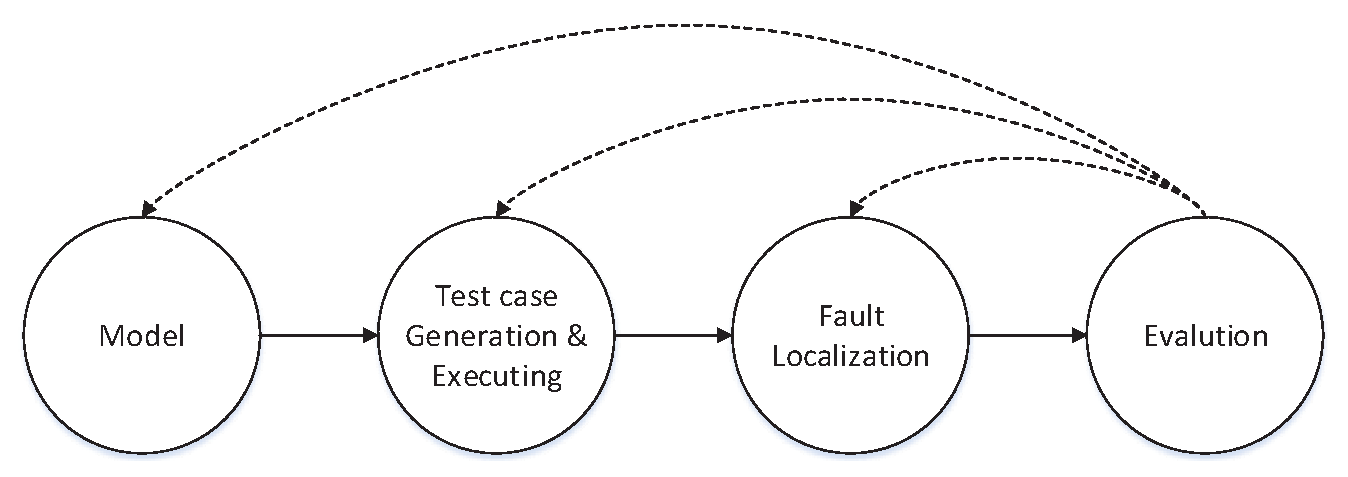
\includegraphics[width=3.4in]{CT_lifecircle.eps}
\caption{The life cycle of CT}
\label{ct-life}
\end{figure}

% An example of a floating figure using the graphicx package.




\section{Background}\label{sec:back}
This section presents some definitions and propositions to give a formal model for CT.

%\subsection{Failure-inducing interactions in CT}

Assume that the Software Under Test (SUT) is influenced by \emph{n} parameters, and each parameter $p_{i}$ can take the values from the finite set $V_{i}$, $|V_{i}|$ = $a_{i}$ ($i$ = 1,2,..n). The definitions below are originally defined in \cite{nie2011minimal}.

\newtheorem{definition}{Definition}
\begin{definition}
A \emph{test case} of the SUT is a tuple of \emph{n} values, one for each parameter of the SUT. It is denoted as  ($v_{1}$, $v_{2}$,...,$v_{n}$), where $v_{1}\in V_{1}$, $v_{2} \in V_{2}$ ... $v_{n} \in V_{n}$.
\end{definition}
%a \emph{n}-tuple

In practice, these parameters in the test case can represent many factors, such as input variables, run-time options, building options or various combination of them. We need to execute the SUT with these test cases to ensure the correctness of the behaviour of the SUT.

%\begin{definition}
We consider any abnormally executing test case as a \emph{fault}. It can be a thrown exception, a compilation error, an assertion failure, a constraint violation, etc. When faults are triggered by some test cases, it is desired to figure out the cause of these faults.
%Some subsets of these test cases should be analysed.
%\end{definition}


\begin{definition}
For the SUT, the \emph{n}-tuple (-,$v_{n_{1}}$,...,$v_{n_{k}}$,...)is called a \emph{k}-degree \emph{schema} ($0 < k \leq n $) when some k parameters have fixed values and other irrelevant parameters are represented as "-".

In effect, a test case itself is a k-degree \emph{schema} when k = n. Furthermore, if a test case contains a \emph{schema}, i.e., every fixed value in the schema is in this test case, we say this test case \emph{contains} the \emph{schema}.
%, which can be denoted as $k-value\  combination \in T$
\end{definition}
Note that the schema is a formal description of the interaction between parameter values we discussed before.

\begin{definition}
Let $c_{l}$ be a \emph{l}-degree schema, $c_{m}$ be an \emph{m}-degree schema in SUT and $l < m$. If all the fixed parameter values in $c_{l}$ are also in $c_{m}$, then $c_{m}$ \emph{subsumes} $c_{l}$. In this case, we can also say that $c_{l}$ is a \emph{sub-schema} of $c_{m}$ and $c_{m}$ is a \emph{super-schema} of $c_{l}$, which can be denoted as $c_{l} \prec  c_{m}$.
\end{definition}

For example,  the 2-degree schema (-, 4, 4, -) is a sub-schema of the 3-degree schema (-, 4, 4, 5), that is, (-,4,4,-) $\prec$ (-,4,4,5).

\begin{definition}
If all test cases that contain a schema, say $c$, trigger a particular fault, say $F$, then we call this schema $c$ the \emph{faulty schema} for $F$. Additionally, if none of sub-schema of $c$ is the \emph{faulty schema} for $F$, we then call the schema $c$ the \emph{minimal failure-causing schema (MFS)} \cite{nie2011minimal} for $F$.

%Based on this, if a test case $t$ hit such a failure-inducing combination, say $c(F)$, it should trigger the fault $F$, for which the test case can be put as $t(F)$
\end{definition}

Note that MFS is identical to the failure-inducing interaction discussed previously. In this paper, the terms \emph{failure-inducing interactions} and \emph{MFS} are used interchangeably. Figuring the MFS out helps to identify the root cause of a failure and thus facilitate the debugging process.

% Note that failures discussed are assumed to be deterministic in this paper. This assumption is a common assumption of CT\cite{zhang2011characterizing,ghandehari2012identifying,niu2013identifying}. It indicates that the outcome of executing a test case is reproducible and will not be affected by some random events. Some approaches have already proposed measures to handle this problem \cite{yilmaz2006covering,fouche2009incremental}.


\subsection{CT Test Case Generation}\label{sec:back:gen}
When applying CT, the most important work is to determine whether the SUT suffers from the interaction faults or not, i.e., to  detect the existence of the MFS. Rather than impractically executing exhaustive test cases, CT commonly designs a relatively small set of test cases to cover all the schemas with the degree no more than a prior fixed number, $t$. Such a set of test cases is called the \emph{covering array}.  If some test cases in the covering array failed in execution, then the interaction faults are considered to be detected. Let us formally define the covering array.

\begin{definition} $MCA(N; t, n,$ $(a_{1}, a_{2}, ..., a_{n})$) is a $t$-way \emph{covering array} in the form of $N \times n$ table, where each row represents a \emph{test case} and each column represents a parameter.  For any \emph{t} columns, each possible \emph{t}-degree interaction of the $t$ parameters (schema) must appear at least once. When $ a_{1} = a_{2} = ... = a_{n} = v $, a $t$-way covering array can be denoted as $CA(N; t, n, v)$.
\end{definition}

\begin{table}[!ht]
\renewcommand{\arraystretch}{1.3}
\caption{A covering array}
\label{ca_example}
\centering
\begin{tabular}{l|llll}
 \hline
ID &\multicolumn{4}{c}{\bfseries Test case} \\  \hline
$t_{1}$ &\multicolumn{4}{l}{0  \ \ \ \  0 \ \ \ \  0 \ \ \ \ 0} \\
$t_{2}$ &\multicolumn{4}{l}{0  \ \ \ \  1 \ \ \ \  1 \ \ \ \ 1} \\
$t_{3}$ &\multicolumn{4}{l}{1  \ \ \ \  0 \ \ \ \  1 \ \ \ \ 1} \\
$t_{4}$ &\multicolumn{4}{l}{1  \ \ \ \  1 \ \ \ \  0 \ \ \ \ 1} \\
$t_{5}$ &\multicolumn{4}{l}{1  \ \ \ \  1 \ \ \ \  1 \ \ \ \ 0} \\
 \hline
\end{tabular}
\end{table}

For example, Table \ref{ca_example} shows a 2-way covering array CA(5; 2, 4, 2) for the SUT with 4 boolean parameters. For any two columns, any 2-degree schema is covered. Covering array has proven to be effective in detecting the failures caused by interactions of parameters of the SUT. Many existing algorithms focus on constructing covering arrays such that the number of test cases, i.e., $N$, can be as small as possible. In general, most of these studies can be classified into three categories according to the construction strategy of the covering array\cite{nie2011survey}:

1) One test case one time: This strategy repeats generating one test case as one row of the covering array and counting the covered schemas achieved until all schemas are covered \cite{cohen1997aetg,bryce2007density,tung2000automating}.

%  generate a completed test case to cover

2) A  set of test cases one time:  This strategy generates a set of test cases at each iteration. Through mutating the values of some parameters of some test cases in this test set, it focuses on optimizing the coverage. If the coverage is finally satisfied, it will reduce the size of the set to see if fewer test cases can still fulfill the coverage. Otherwise, it will increase the size of the test set to cover all the schemas\cite{cohen2003augmenting,nurmela2004upper}.

3) IPO-like style:  This strategy differentiates from the previous two strategies in that it does not firstly generate complete test cases \cite{lei2008ipog}. Instead, it first focuses on assigning values to some part of the factors or parameters to cover the schemas that are related to these factors, and then fills up the remaining part to form complete test cases.

In this paper, we focus on the first strategy: One test case one time as it immediately gets a complete test case so that the testers can execute and diagnose in the early stage. As we will see later, with respect to the MFS identification, this strategy is the most flexible and efficient one compared with the other two strategies.

%To isolate the failure-inducing schemas and further bug fixing, the first step, is to detect them. To efficiently isolate the failure-inducing schemas, and to . Such a testing object, is covering array, which ,. Formally,
%
%\begin{definition}
%Covering array.
%\end{definition}

%Such a covering can , how to generate such a covering lying two facts.
%There are three different kinds of generation
%
%Overall test
%
%one test one time
%
%other special testing object.

%In order to fulfil the testing target, we choose the second object, one test one time, as we can .

\subsection{Identify the failure-inducing interactions}\label{sec:back:iden}
To detect the existence of MFS in the SUT is still far from figuring out the root cause of the failure \cite{colbourn2008locating,martinez2008algorithms,martinez2009locating}, as we do not know exactly which schemas in the failed test cases should be responsible for the failure. For example, if $t_{1}$ in Table \ref{ca_example} failed during testing, there are six 2-degree candidate failure-inducing schemas, which are (0, 0, -, -), (0, -, 0, -), (0, -, -, 0) , (-, 0, 0, -), (-, 0, -, 0), (-, -, 0, 0), respectively. Without
additional information, it is difficult to figure out the specific schemas in this suspicious set that caused the failure. Considering that the failure can be triggered by schemas with other degrees, e.g., (0, -, -, -) or (0, 0, 0, -), the problem of MFS identification becomes more complicated.

In fact, for a failing test case ($v_{1},v_{2},...,v_{n}$), there can be at most $2^{n} - 1$ possible schemas for the MFS. Hence, more test cases should be generated to identify the MFS. In CT, the main work in fault localization is to identify the failure-inducing interactions. So in this paper, we only focus on the MFS identification. Further works of fault localization such as isolating the specific defective source code will not be discussed.

A typical MFS identification process is shown in Table \ref{ofot-identify}. This example assumes the SUT has 3 parameters, each of which can take on 2 values, and the test case (1, 1, 1) fails. Then in Table \ref{ofot-identify}, as test case \emph{t} failed, we mutate one factor of test case \emph{t} one time to generate new test cases: $t_{1}$ -- $t_{3}$, It turns out that test case $t_{1}$ passed, which indicates that this test case breaks the MFS in the original test case \emph{t}. So (1,-,-) should be a failure-causing factor. Besides, since other mutating test cases all failed, there is no any other failure-inducing factor that is broken. Therefore, the MFS in \emph{t} is (1,-,-).

\begin{table}[!t]
\caption{OFOT example}
\label{ofot-identify}
\centering
\begin{tabular}{llllll}
 \hline
\multicolumn{5}{c}{\bfseries Original test case} & \bfseries Outcome \\  \hline
 $t$ & \multicolumn{4}{l}{1 \ \ \ \ 1 \ \ \ \  1 } & Fail \\
 \hline
\multicolumn{5}{c}{\bfseries Additional  test cases} &  \\  \hline
$t_{1}$ &\multicolumn{4}{l}{0  \ \ \ \  1 \ \ \ \  1 }& Pass \\
$t_{2}$ &\multicolumn{4}{l}{1  \ \ \ \  0 \ \ \ \  1 } & Fail \\
$t_{3}$ &\multicolumn{4}{l}{1  \ \ \ \  1 \ \ \ \  0 } & Fail \\
 \hline
\end{tabular}
\end{table}

This identification process mutate one factor of the original test case at a time to generate extra test cases. Then according to the outcome of the test cases execution result, it will identify the MFS of the original failing test cases. It is called the OFOT method \cite{nie2011minimal}, which is a well-known MFS identification method in CT. In this paper, we will focus on this identification method. It should be noted that the following proposed CT framework can be easily applied to other MFS identification methods.

Note that all the existing MFS identification approaches just give approximation solutions for MFS identification. In fact, to exactly identify the MFS (without any assumptions), it needs exponential number of test cases \cite{niu2013identifying}, which is impossible in practice. Hence, all the existing MFS identification approaches, as well as the approach we will propose in this paper, need additional assumptions or just identify the likely failure-inducing interactions. For example, the OFOT approach is based on the following two assumptions:
\newtheorem{assumption}{Assumption}
\begin{assumption}  The execution result of a test case is deterministic.
\end{assumption}

This assumption is a common assumption of CT\cite{zhang2011characterizing,ghandehari2012identifying,niu2013identifying}. It indicates that the outcome of executing a test case is reproducible and will not be affected by some random events.

\begin{assumption}
Given a failing test case $t$, when we identify the MFS in $t$, any newly generated test case will not introduce new MFS that is not in $t$.
\end{assumption}

The second assumption is identical to the assumption proposed in \cite{zhang2011characterizing,martinez2008algorithms,martinez2009locating}, which is called the safe value assumption. Based on this assumption, when the additional test case generated by OFOT fails, e.g., $t_{2}$ in Table \ref{ofot-identify}, we can determine that the additional test case contains the same MFS in the original failing test case, e.g., $t$ in Table \ref{ofot-identify}.

Note that in practice, these assumptions do not always hold. Hence, the approaches proposed later in this paper actually can only identify approximate MFS instead of the real MFS. We will discuss the impacts of these assumptions on the approaches proposed in this paper in the experiments. \textbf{Additionally, without special emphasis (for example, ��the real MFS��), all the sentences contained such as "the MFS identified by some approaches" actually mean that "the approximate MFS obtained by these approaches".}

\section{Motivating example}\label{sec:moti}
In this section, a motivating example is presented to show how traditional CT works as well as its limitations. This example is derived from our attempt to test a real-world software--HSQLDB, which is a pure-java relational database engine with large and complex configuration space. To extract and manipulate valid configurations of this highly-configurable system is important, as different configurations can result in significantly different behaviours of the system \cite{jin2014configurations,qu2008configuration,song2012itree} (HSQLDB normally works under some proper configurations, but crashes or throws exceptions under some other configurations).

%reduce the space, or give an description
Considering the large configuration space of HSQLDB, we first utilized CT to generate a relatively small set of test cases. Each of them is actually a set of specific assignments to those options we cared  \footnote{More details in: http://gist.nju.edu.cn/doc/ict/}. For each configuration, HSQLDB is tested by sending prepared SQL commands. We recorded the output of each run, but unfortunately, about half of them produced exceptions or warnings. Following the schedule of traditional CT, we started the identification process to isolate the failure-inducing option interactions in those failing configurations. Each failing configuration should be individually handled, in principle, as there may exist distinct failure-inducing option interactions among them. However, this successive identification process, although appealing, was hardly ever followed for this case study. This is because there are too many failing configurations and most of them contain the same failure-inducing option interactions, based on which the MFS identification process is wasteful and inefficient.

For the sake of convenience, we provide a highly simplified scenario to illustrate the problems we encountered. Consider four options in HSQLDB -- \emph{Server type}, \emph{Scroll Type}, \emph{Parameterised SQL} and \emph{Statement Type}.  The possible values each option can take on are shown in Table \ref{tomcat-simplifiy}. Based on the report in the bug tracker of HSQLDB \footnote{For details, see: http://sourceforge.net/p/hsqldb/bugs/1173/}, an \emph{incompatible exception} will be triggered if a \emph{parameterised sql} is executed as \emph{prepared statement} by HSQLDB. Hence, when option $ parameterised SQL$ is set to be \emph{true} and $Statmetent$ to be \emph{preparedStatement}, our testing will crash. Besides this failure, there exists another option value which can also crash this database engine. It is when \emph{Scroll Type} is assigned to \emph{sensitive}, as this feature is not supported by this version of HSQLDB \footnote{For details, see: http://hsqldb.org/doc/guide/guide.html}. Without this knowledge at prior, we need to detect and isolate these two failure-inducing option interactions by CT.

%Table \ref{tradition-gi} presents such process. Note that every possible combinations of is covered by at least one test case, for example, every possible combination of the values for options can be find at least one test case. Then as expected, test case 1, 4, 7 are failed because they either contain failure-interaction or the contraint option .  Then we need to identify the failure-inducing interactions for each failing test case using OFOT. This procss is shown in  \emph{identification} part of Table \ref{tradition-gi}.
%

%Another option that can make . However, this . In this example, we deemed them as the same, as they all can make the testing unproceeball.

\begin{table}[ht]
\caption{Highly simplified configuration of HSQLDB}
\label{tomcat-simplifiy}
\centering
\begin{tabular}{cc|ccccc}
 \hline
 \multicolumn{2}{c}{\bfseries Option} & \multicolumn{5}{c}{\bfseries Values} \\  \hline
$o_{1}$ & Server type & \multicolumn{5}{c}{ server, web-server, in-process} \\
$o_{2}$ & Scroll type & \multicolumn{5}{c}{ sensitive,insensitive, forward-only} \\
$o_{3}$ & parameterised SQL & \multicolumn{5}{c}{true, false} \\
$o_{4}$ & Statement Type & \multicolumn{5}{c}{ statement, preparedStatement} \\
 \hline
\end{tabular}
\end{table}


Table \ref{tradition-gi} illustrates the process of traditional CT on this subject. For simplicity of notation, we use consecutive symbols 0, 1, 2 to represent different values of each option (For $parameterised SQL$ and $Statement$, the symbol is up to 1). According to Table \ref{tradition-gi}, traditional CT first generated and executed the 2-way covering array ($t_{1}$ -- $t_{9}$ in the \emph{generation} part). Note that this covering array covered all the 2-degree schemas for the SUT.
%For example, all the possible values combinations between first and second parameters appear at least one test case.

After testing with the 9 test cases ($t_{1}$ to $t_{9}$),  we found $t_{1}$, $t_{4}$, and $t_{7}$ failed. It is then desired to respectively identify the MFS of these failing test cases. For $t_{1}$, OFOT method is used to generate four additional test cases ($t_{10}$ -- $t_{13}$), and the MFS (-, 0, - , -) of $t_{1}$ is identified (\emph{Scroll Type} is assigned to \emph{sensitive}, respectively). This is because only when changing the second factor of $t_{1}$, the additionally generated test case will pass. Then the same process is applied on $t_{4}$ and $t_{7}$. Finally, we found that the MFS of $t_{4}$ is (-, -, -, -), indicating that OFOT failed to determine the MFS (this will be discussed later), and the MFS of $t_{7}$ is the same as $t_{1}$. Totally, for detecting and identifying the MFS in this example, we generated 12 additional test cases (marked with stars).

\begin{table}[ht]
\caption{Sequential CT process}
\label{tradition-gi}
\centering
\begin{tabular}{lllllll}
%\cline{2-7}
                                       & \multicolumn{6}{c}{\bfseries \emph{Generation (Execution)}}                                                                                                                                                                                                                                  \\ \cline{2-7}
                                       & \multicolumn{5}{c|}{\bfseries test case}                                                                                                                                                                                                              & \bfseries Outcome \\
                                       & &$o_{1}$ & $o_{2}$& $o_{3}$& \multicolumn{1}{c|}{$o_{4}$}&  \\    \cline{2-7}
                                       & \multicolumn{1}{l|}{$t_{1}$}   & 0& \textbf{0}& 0& \multicolumn{1}{l|}{0}     & Fail              \\
                                       & \multicolumn{1}{l|}{$t_{2}$}   & 0& 1& 1& \multicolumn{1}{l|}{1}     & Pass              \\
                                       & \multicolumn{1}{l|}{$t_{3}$}   & 0& 2& 1& \multicolumn{1}{l|}{0}     & Pass              \\
                                       & \multicolumn{1}{l|}{$t_{4}$}   & 1& \textbf{0}& \textbf{0}& \multicolumn{1}{l|}{\textbf{1}}     & Fail              \\
                                       & \multicolumn{1}{l|}{$t_{5}$}   & 1& 1& 0& \multicolumn{1}{l|}{0}     & Pass              \\
                                       & \multicolumn{1}{l|}{$t_{6}$}   & 1& 2& 1& \multicolumn{1}{l|}{1}     & Pass              \\
                                       & \multicolumn{1}{l|}{$t_{7}$}   & 2& \textbf{0}& 1& \multicolumn{1}{l|}{1}     & Fail              \\
                                       & \multicolumn{1}{l|}{$t_{8}$}   & 2& 1& 0& \multicolumn{1}{l|}{0}     & Pass              \\
                                       & \multicolumn{1}{l|}{$t_{9}$}   & 2& 2& 0& \multicolumn{1}{l|}{0}     & Pass              \\ \cline{2-7}
                                       \multicolumn{6}{c}{} \\
                                       & \multicolumn{6}{c}{\bfseries \emph{Identification}}                                                                                                                                                                                                                              \\ \cline{2-7}
\multicolumn{1}{l|}{\multirow{5}{*}{\rotatebox{90}{$t_{1}$ (0,0,0,0)}}} & \multicolumn{1}{l|}{$t_{10}$*} & 1& 0& 0& \multicolumn{1}{l|}{0} & Fail              \\
\multicolumn{1}{l|}{}                  & \multicolumn{1}{l|}{$t_{11}$*} & 0& 1& 0& \multicolumn{1}{l|}{0} & Pass              \\
\multicolumn{1}{l|}{}                  & \multicolumn{1}{l|}{$t_{12}$*} & 0& 0& 1& \multicolumn{1}{l|}{0} & Fail              \\
\multicolumn{1}{l|}{}                  & \multicolumn{1}{l|}{$t_{13}$*} & 0& 0& 0& \multicolumn{1}{l|}{1} & Fail              \\ \cline{2-7}
\multicolumn{1}{l|}{}                  & \multicolumn{1}{l|}{\bfseries MFS} & \multicolumn{5}{c}{\bfseries   (-, 0, -, -)}                                                                                                                                                                                                                 \\  \cline{2-7}
                                   %    \multicolumn{6}{c}{} \\
                                       %\cline{2-7}
\multicolumn{1}{l|}{\multirow{5}{*}{\rotatebox{90}{$t_{4}$ (1,0,0,1)}}} & \multicolumn{1}{l|}{$t_{14}$*} & 2& \textbf{0}& \textbf{0}& \multicolumn{1}{l|}{\textbf{1}} & Fail              \\
\multicolumn{1}{l|}{}                  & \multicolumn{1}{l|}{$t_{15}$*} & 1& 1& \textbf{0}& \multicolumn{1}{l|}{\textbf{1}} & Fail              \\
\multicolumn{1}{l|}{}                  & \multicolumn{1}{l|}{$t_{16}$*} & 1& \textbf{0}& 1& \multicolumn{1}{l|}{1} & Fail              \\
\multicolumn{1}{l|}{}                  & \multicolumn{1}{l|}{$t_{17}$*} & 1& \textbf{0}& 0& \multicolumn{1}{l|}{0} & Fail              \\ \cline{2-7}
\multicolumn{1}{l|}{}                  & \multicolumn{1}{l|}{\bfseries MFS} & \multicolumn{5}{c}{\bfseries   (-, -, -, -)}                                                                                                                                                                                                                 \\  \cline{2-7}
                                      %  \multicolumn{6}{c}{} \\
                                %        \cline{2-7}
\multicolumn{1}{l|}{\multirow{5}{*}{\rotatebox{90}{$t_{7}$ (2,0,1,1)}}} & \multicolumn{1}{l|}{$t_{18}$*} & 0& 0& 1& \multicolumn{1}{l|}{1} & Fail              \\
\multicolumn{1}{l|}{}                  & \multicolumn{1}{l|}{$t_{19}$*} & 2& 1& 1& \multicolumn{1}{l|}{1} & Pass              \\
\multicolumn{1}{l|}{}                  & \multicolumn{1}{l|}{$t_{20}$*} & 2& 0& 0& \multicolumn{1}{l|}{1} & Fail              \\
\multicolumn{1}{l|}{}                  & \multicolumn{1}{l|}{$t_{21}$*} & 2& 0& 1& \multicolumn{1}{l|}{0} & Fail              \\ \cline{2-7}
\multicolumn{1}{l|}{}                  & \multicolumn{1}{l|}{\bfseries MFS} & \multicolumn{5}{c}{\bfseries   (-, 0, -, -)}                                                                                                                                                                                                                 \\  \cline{2-7}
\end{tabular}
\end{table}


We refer to such traditional life-cycle as \emph{\textbf{Sequential CT}} (SCT). However, we believe this may not be the best choice in practice. The first reason is that the engineers normally do not want to wait for fault localization after all the test cases are executed. The early bug fixing is appealing and can give the engineers confidence to keep on improving the quality of the software. The second reason, which is also more important, is such life-cycle can generate many redundant and unnecessary test cases, which negatively impacted on both test case generation and MFS identification.
The most obvious negative effect in this example is that we did not identify the expected failure-inducing interaction (-, -, 0, 1), which corresponds to option $ parameterised SQL$ being set to \emph{true} and $Statmetent$ to \emph{preparedStatement}. More shortcomings of the sequential CT are discussed as follows:

\subsection{Redundant test cases}\label{sec:moti:redu}
The first shortcoming of SCT is that it may generate redundant test cases so that some of them do not cover as many uncovered schemas as possible. As a consequence, SCT may generate more test cases than actually needed. This can be reflected in the following two aspects:

1) The test cases generated in the identification stage can also contribute some coverage, i.e., the schemas appear in the passing test cases in the identification stage may have already been covered in the test case generation stage. For example, when we identify the MFS of $t_{1}$ in Table \ref{tradition-gi}, the schema (0, 1, -, -) contained in the extra passing test case $t_{11}$ -- (0, 1, 0, 0) has already appeared in the passing test case $t_{2}$ -- (0, 1, 1, 1). In other words, if we first identify the MFS of $t_{1}$, then $t_{2}$ is not a good choice as it does not cover as many 2-degree schemas as possible. For example, (1, 1, 1, 1) is better than this test case at contributing more coverage.

2)The identified MFS should not appear in the following generated test cases.  This is because according to the definition of MFS, each test case containing this schema will trigger a failure, i.e., to generate and execute more than one test case contained the MFS makes no sense for the failure detection. Taking the example in Table \ref{tradition-gi}, after identifying the MFS -- (-, 0, -, -) of $t_{1}$, we should not generate the test case $t_{4}$ and $t_{7}$. This is because they also contain the identified MFS (-, 0, -, -), which will result in them failing as expected. Since the expected failure caused by MFS (-, 0, -, -) makes $t_{7}$ and $t_{9}$ superfluous for error-detection, the additional test cases ($t_{14}$ to $t_{21}$) generated for identifying the MFS in $t_{4}$ and $t_{7}$ are also not necessary.


\subsection{Multiple MFS in the same test case}\label{sec:moti:multi}
When there are multiple MFS in the same test case, MFS identification will be negatively affected. Particularly, some MFS identification approaches can not identify a valid schema in this case. For example, there are two MFS in $t_{4}$ in Table \ref{tradition-gi}, i.e., (-, 0, -, -) and (-, -, 0, 1) (shown in bold). When we use OFOT method, we found all the additionally generated test cases ($t_{14}$ to $t_{17}$) failed. These outcomes give OFOT a false indication that all the failure-inducing factors are not broken by mutating those four parameter values.  As a result, OFOT cannot determine which schemas are MFS, which is denoted as (-, -, -, -).

The reason why OFOT cannot properly work is that this approach can only break one MFS at a time. If there are multiple MFS in the same test case, the additionally generated test cases will always fail as they contain other non-broken MFS (see bold parts of $t_{14}$ to $t_{17}$). Some approaches have been proposed to handle this problem, but they either cannot handle multiple MFS that have overlapping parts \cite{zhang2011characterizing}, or consume too many additionally generated test cases \cite{wang2010adaptive,niu2013identifying}. So in practice, to make MFS identification more effective and efficient, we need to avoid the appearance of multiple MFS in the same test case.

SCT, however, does not offer much support for this concern. This is mainly because it is essentially a post-analysis framework, i.e., the analysis for MFS comes after the completion of test case generation and execution. As a result, in the generation stage, testers have no knowledge of the possible MFS, and surely it is possible that multiple MFS appear in the same test case.
%
%SCT, however, will increase the chance that multiple MFS appear in one test case. This is because the .
%
\subsection{Masking effects}\label{sec:moti:mask}
 When considering a single execution of the test set, traditional covering array usually offer an inadequate testing due to \emph{Masking effects} \cite{dumlu2011feedback,yilmaz2013reducing}. A masking effect\cite{yilmaz2013reducing} is an effect that some failures or exceptions prevent a test case from testing all valid schemas in that test case, which the test case is normally expected to test. For example in Table \ref{tradition-gi}, $t_{1}$ is initially expected to cover six 2-degree schemas, i.e., (0, 0, - , -), (0, -, 0, -), (0, -, -, 0), (-, 0, 0, -), (-, 0, -, 0), and (-, -, 0, 0), respectively. The failure of this test case, however, may prevent the checking of these schemas. This is because, the failing of $t_{1}$ ($Scroll Type$ is set to be $sensitive$) crashed HSQLDB, and as a result, it did not go on executing the remaining test code, which may affect the examination of some interactions of $t_{1}$. Hence, we cannot ensure we have thoroughly exercised all the interactions in this failing test case.


Since traditional covering array alone cannot reach an adequate testing, as an alternative, \emph{tested t-way interaction criterion} as a more rigorous coverage standard is proposed \cite{yilmaz2013reducing}. According to this criterion, a $t$-degree schema is covered iff (1) it appears in a passing test case, or (2) it is identified as MFS or faulty schema. Apparently, this criterion can not be satisfied with traditional covering array alone (in practice, it is often the case that the test set is rerun until all test cases pass). Next let us examine whether this criterion can be satisfied with SCT, i.e., the combination of traditional covering array and MFS identification.

One obvious insight is that if there is only \textbf{single} MFS in each failing test case, this criterion is satisfied. This conclusion is based on the fact that the MFS identification is actually a process to isolate the failure-inducing interaction among other interactions in the failing test case,  and since there is only a single MFS, then other schemas can be determined as non-MFS.

For example in Table \ref{tradition-gi}, $t_{1}$ contained a single MFS (-, 0, -, -), and we identified this MFS by generating four extra test cases ($t_{10}$ to $t_{13}$). As for $t_{1}$, the schema (-, 0, -, -) is determined to be MFS, but since the target of that testing is $2$-way coverage, i.e., to cover all the 2-degree schemas, this $1$-degree schema does not contribute any more coverage. Based on the fact that (-, 0, -, -) is MFS, all the test cases containing this schema will fail by definition, and surely the super-schemas of (-, 0, -, -) in this test case -- (0, 0, -, -), (-, 0, 0, -) and (-, 0, -, 0) are also faulty schemas as all the test cases containing these schemas must contain the MFS (-, 0, -, -), which will fail after execution. The remaining 2-degree schemas (0, -, 0, -), (0, -, -, 0), (-, -, 0, 0) are contained in the additionally generated test case $t_{11}$ (0, 1, 0, 0) (Note that for single MFS, there will be at least one passing additionally generated test case ), which are of course non-faulty schemas.  After all, all the 2-degree schemas in the failing test case $t_{1}$ satisfied the \emph{tested t-way interaction criterion}.

When a failing test case has \textbf{multiple} MFS, however, SCT fails to meet that criterion. As discussed previously, SCT cannot properly work on test cases with multiple MFS--and even cannot obtain a valid schema. With this in mind, we cannot determine which schemas in this failing test case are MFS or not. Consequently, we cannot ensure we have examined all the $t$-degree schemas in this failing test case. For example, $t_{4}$ has two MFS--(-, 0, -, -), (-, -, 0, 1), which can not be identified with OFOT approach (In fact, there is no passing additionally generated test case). As a result, there are two 2-degree schemas (1, 0, -, -) (-, -, 0, 1) in this test case that are neither contained in a passing test case nor determined as MFS or faulty schemas.  Hence, \emph{tested t-way interaction criterion} is not satisfied.  Since multiple MFS in a test case can introduce masking effects, SCT must be negatively affected as it lacks mechanisms to avoid the appearance of multiple MFS in failing test cases.

Note that the \emph{masking effects} are actually caused by the \emph{multiple MFS problem} we discussed previously. But these two problems focus on different aspects of combinatorial testing. The \emph{masking effects} mainly focus on the test sufficiency of CT, which can be regarded as a metric to evaluate how many schemas are actually tested \cite{yilmaz2013reducing}. While for \emph{multiple MFS problem}, it mainly focuses on the quality of MFS identification. To be convenient, we separately discuss these two problems later in this paper.

%\begin{table}[h]
%\caption{The satisfaction of tested t-way interaction criterion}
%\label{ofot-proof}
%\center
%\begin{tabular}{llllll}
% \hline
%\multicolumn{5}{c}{\bfseries Original test case} & \bfseries Outcome \\  \hline
% $t$ & \multicolumn{4}{l}{1 \ \ \ \ 1 \ \ \ \  1 } & Fail \\
% \hline
%\multicolumn{5}{c}{\bfseries Additional  test cases} &  \\  \hline
%$t_{1}$ &\multicolumn{4}{l}{0  \ \ \ \  1 \ \ \ \  1 }& Pass \\
%$t_{2}$ &\multicolumn{4}{l}{1  \ \ \ \  0 \ \ \ \  1 } & Fail \\
%$t_{3}$ &\multicolumn{4}{l}{1  \ \ \ \  1 \ \ \ \  0 } & Fail \\
% \hline
%\end{tabular}
%\end{table}

%This is mainly caused after the second.
%
%Even worse, such test case may suffer from the \emph{masking effects} \cite{yilmaz2013reducing}, as failures caused by the already identified MFS can prevent the test case from normally checked (e.g., failures that can trigger an unexpected halt of the execution). As a result, some schemas in these test cases that are supposed to be examined will actually skip the testing.
%
%and even worse some other schemas in $t_{4}$ or $t_{7}$  may be masked, as those schemas can potentially trigger other failures but will not be observed.


%This section presents the .
%As discussed previously, the generation and identification are the most important stages in CT life-cycle. How to enhance these two activities in the CT life-cycle is of importance as it greatly impacts on the quality and cost of overall software testing. In fact, most studies in CT focus on these two fields. But rather than as a whole, generation and identification are applied independently. The justification for not discussing how to cooperate these two activities is that the first-generation-then-identification is so natural and straightforward. As we will show below, however, that the generation and identification is so tightly correlated that they have a significant impact on the effectiveness and efficiencies of testing.
%\subsection{Summary of the motivation example}
%
%Based on these observations, a more effective and efficient framework is desired.


\subsection{Augmentation of the SCT}

Considering the fact that we do not need to repeatedly identify the same MFS, we can reduce the number of test cases by checking the already identified MFS and removing it from the MFS identification process. For example in Table \ref{tradition-gi}, we do not need to generate 4 additional test cases ($t_{18}$ to $t_{21}$) to figure out the failure-cause of $t_{7}$ is indeed (-, 0, -, -), which has already been identified in previous iteration ($t_{10}$ to $t_{13}$). Therefore, we only need to check whether there is any MFS other than (-, 0, -, -) in $t_{7}$ or not. When applying this augmentation, the overall SCT process of the example in Table \ref{tradition-gi} will evolve into the process shown in Table \ref{tradition-gi-aug}.


\begin{table}[ht]
\caption{Augmented Sequential CT process}
\label{tradition-gi-aug}
\centering
\begin{tabular}{lllllll}
%\cline{2-7}
                                       & \multicolumn{6}{c}{\bfseries \emph{Generation (Execution)}}                                                                                                                                                                                                                                  \\ \cline{2-7}
                                       & \multicolumn{5}{c|}{\bfseries test case}                                                                                                                                                                                                              & \bfseries Outcome \\
                                       & &$o_{1}$ & $o_{2}$& $o_{3}$& \multicolumn{1}{c|}{$o_{4}$}&  \\    \cline{2-7}
                                       & \multicolumn{1}{l|}{$t_{1}$}   & 0& \textbf{0}& 0& \multicolumn{1}{l|}{0}     & Fail              \\
                                       & \multicolumn{1}{l|}{$t_{2}$}   & 0& 1& 1& \multicolumn{1}{l|}{1}     & Pass              \\
                                       & \multicolumn{1}{l|}{$t_{3}$}   & 0& 2& 1& \multicolumn{1}{l|}{0}     & Pass              \\
                                       & \multicolumn{1}{l|}{$t_{4}$}   & 1& \textbf{0}& \textbf{0}& \multicolumn{1}{l|}{\textbf{1}}     & Fail              \\
                                       & \multicolumn{1}{l|}{$t_{5}$}   & 1& 1& 0& \multicolumn{1}{l|}{0}     & Pass              \\
                                       & \multicolumn{1}{l|}{$t_{6}$}   & 1& 2& 1& \multicolumn{1}{l|}{1}     & Pass              \\
                                       & \multicolumn{1}{l|}{$t_{7}$}   & 2& \textbf{0}& 1& \multicolumn{1}{l|}{1}     & Fail              \\
                                       & \multicolumn{1}{l|}{$t_{8}$}   & 2& 1& 0& \multicolumn{1}{l|}{0}     & Pass              \\
                                       & \multicolumn{1}{l|}{$t_{9}$}   & 2& 2& 0& \multicolumn{1}{l|}{0}     & Pass              \\ \cline{2-7}
                                       \multicolumn{6}{c}{} \\
                                       & \multicolumn{6}{c}{\bfseries \emph{Identification}}                                                                                                                                                                                                                              \\ \cline{2-7}
\multicolumn{1}{l|}{\multirow{5}{*}{\rotatebox{90}{$t_{1}$ (0,0,0,0)}}} & \multicolumn{1}{l|}{$t_{10}$*} & 1& 0& 0& \multicolumn{1}{l|}{0} & Fail              \\
\multicolumn{1}{l|}{}                  & \multicolumn{1}{l|}{$t_{11}$*} & 0& 1& 0& \multicolumn{1}{l|}{0} & Pass              \\
\multicolumn{1}{l|}{}                  & \multicolumn{1}{l|}{$t_{12}$*} & 0& 0& 1& \multicolumn{1}{l|}{0} & Fail              \\
\multicolumn{1}{l|}{}                  & \multicolumn{1}{l|}{$t_{13}$*} & 0& 0& 0& \multicolumn{1}{l|}{1} & Fail              \\ \cline{2-7}
\multicolumn{1}{l|}{}                  & \multicolumn{1}{l|}{\bfseries MFS} & \multicolumn{5}{c}{\bfseries   (-, 0, -, -)}                                                                                                                                                                                                                 \\  \cline{2-7}
                                   %    \multicolumn{6}{c}{} \\
                                       %\cline{2-7}
\multicolumn{1}{l|}{\multirow{5}{*}{\rotatebox{90}{$t_{4}$ (1,0,0,1)}}} & \multicolumn{1}{l|}{\cellcolor{black!25}$t_{14}$*} & \cellcolor{black!25}1& \cellcolor{black!25}1 & \cellcolor{black!25}0& \multicolumn{1}{l|}{\cellcolor{black!25}1} & \cellcolor{black!25}Fail              \\
\multicolumn{1}{l|}{}                  & \multicolumn{1}{l|}{$t_{15}$*} & 2& 1& 0& \multicolumn{1}{l|}{1} & Fail              \\
\multicolumn{1}{l|}{}                  & \multicolumn{1}{l|}{$t_{16}$*} & 1& 2& 0& \multicolumn{1}{l|}{1} & Fail              \\
\multicolumn{1}{l|}{}                  & \multicolumn{1}{l|}{$t_{17}$*} & 1& 1& 1& \multicolumn{1}{l|}{1} & Pass              \\
\multicolumn{1}{l|}{}                  & \multicolumn{1}{l|}{$t_{18}$*} & 1& 1& 0& \multicolumn{1}{l|}{0} & Pass              \\ \cline{2-7}
\multicolumn{1}{l|}{}                  & \multicolumn{1}{l|}{\bfseries MFS} & \multicolumn{5}{c}{\bfseries   (-, -, 0, 1)}                                                                                                                                                                                                                 \\  \cline{2-7}
                                      %  \multicolumn{6}{c}{} \\
                                %        \cline{2-7}
\multicolumn{1}{l|}{\multirow{5}{*}{\rotatebox{90}{$t_{7}$ (2,0,1,1)}}} & \multicolumn{1}{l|}{\cellcolor{black!25}$t_{19}$*} & \cellcolor{black!25}2& \cellcolor{black!25}1 & \cellcolor{black!25}1& \multicolumn{1}{l|}{\cellcolor{black!25}1} & \cellcolor{black!25}Pass              \\
\multicolumn{1}{l|}{}                  & \multicolumn{1}{l|}{} & & & & \multicolumn{1}{l|}{} &               \\
\multicolumn{1}{l|}{}                  & \multicolumn{1}{l|}{} & & & & \multicolumn{1}{l|}{} &               \\
\multicolumn{1}{l|}{}                  & \multicolumn{1}{l|}{} & & & & \multicolumn{1}{l|}{} &               \\
\multicolumn{1}{l|}{}                  & \multicolumn{1}{l|}{} & & & & \multicolumn{1}{l|}{} &               \\  \cline{2-7}
\end{tabular}
\end{table}

In Table \ref{tradition-gi-aug}, the only difference from Table \ref{tradition-gi} is that for test case $t4$ and $t_{7}$, we first checked whether there is any MFS other than the already identified MFS (-, 0, -, -). Hence we generated two additional test cases $t_{14}$ and $t_{19}$ (highlighted), which exclude the MFS (-, 0, -, -) from the original failing test cases $t4$ and $t_{7}$.  Note that $t_{14}$ (1, 1, 0, 1) was generated by mutating the value of the second parameter  of test case $t_{4}$  (1, 0, 0, 1) from 0 to 1(but it also can be any value different from the original value 0 in the test case $t_{4}$ ), and as a result, it removed the previously identified MFS (-,0,-,-). The same as $t_{14}$, $t_{19}$ (2, 1, 1, 1) was also generated  by mutating the value of the second parameter of test case $t_{7}$ (2, 0, 1, 1) from 0 to 1.  We then found that $t_{14}$ still failed after execution, which indicates that $t_{14}$ contains other different MFS, and we continued to use OFOT to identify the MFS of $t_{14}$ and obtained the second MFS (-, -, 0, 1). With respect to $t_{19}$, we found it passed after execution, and hence there is no other MFS in this test case, and we do not need to generate additional test cases. As a result, we have reduced 2 test cases in total by using the augmented SCT.

Although the augmented SCT can reduce the redundancy of test cases to some extent, there still remain some issues, e.g., multiple MFS, and masking effects, that it cannot deal with.


\section{Interleaving Approach}\label{sec:app}

Considering these deficiencies of SCT, we do not need to cover all t-wise interactions before moving to the debugging phase. As an alternative, it is better to make test case generation and MFS identification more closely cooperate with each other. Hence, we propose a new CT generation-identification framework -- \emph{\textbf{Interleaving CT}} (ICT). Our new framework aims at enhancing the interaction of generation and identification to reduce the unnecessary and invalid test cases discussed previously. In other words, the ultimate goal of this framework is to better support MFS identification and test case generation, so that both of them can alleviate the three problems we discussed in Section \ref{sec:moti}.


\subsection{Overall framework}\label{sec:app:frame}
 The basic outline of our framework is illustrated in Figure \ref{new-life}.
\begin{figure}
 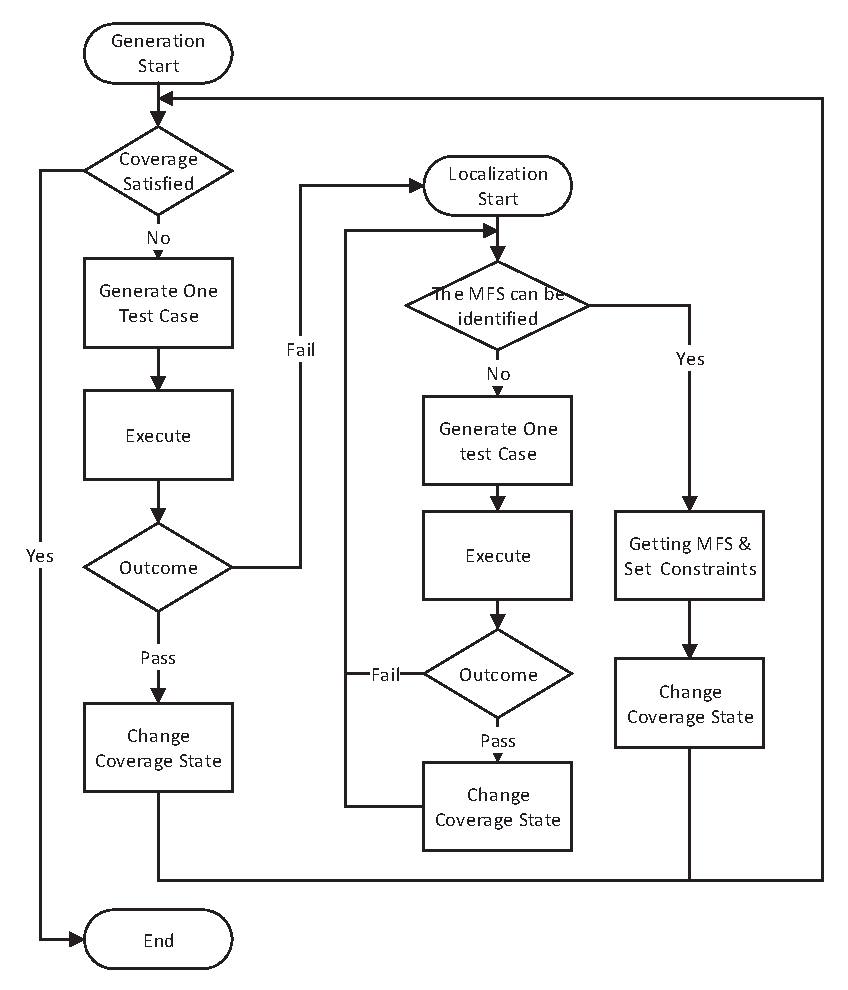
\includegraphics[width=3.4in]{baicOutline.eps}
\caption{The Interleaving Framework}
\label{new-life}
\end{figure}
Specifically, this new framework works as follows: First, it checks whether all the needed schemas are covered or not. Normally the target of CT is to cover all the $t$-degree schemas, with $t$ assigned as 2 or 3. If the current coverage is not satisfied, it will generate a new test case to cover as many uncovered schemas as possible. After that, it will execute this test case with the outcome of a pass (executed normally, i.e., does not trigger an exception, violate the expected Oracle  or the like) or a fail (on the contrary). When the test case passes, we will update the coverage state, as all the schemas in the passing test case are regarded as error-irrelevant. As a result, the schemas that were not covered before will be determined to be covered if it is contained in this newly generated test case. Otherwise, if the test case fails, then we will start the MFS identification module to identify the MFS in this failing test case. One point to note is that if the test case fails, we will not directly change the coverage, as we can not figure out which schemas are responsible for this failure among all the schemas in this test case until we identify them.

The identification module works in a similar way as traditional independent MFS identification process, i.e., repeats generating and executing additional test cases until it can get enough information to diagnose the MFS in the original failing test case. The difference from traditional MFS identifying process is that we record the coverage that this module has contributed to the overall coverage. In detail, when the additional test case passes, we will label the schemas in these test cases as covered if it has not been covered before. When the MFS is found at the end of this module, we will first set them as forbidden schemas that later generated test cases should not contain (Otherwise, the test case must fail and it cannot contribute to more coverage), and second, all the $t$-degree schemas that are \emph{related} to these MFS as covered. Here the \emph{related} schemas indicate the following three types of $t$-degree schemas:

First, the MFS \textbf{themselves}. Note that we do not change the coverage state after the generated test case fails (both for the generation and identification module ), so these MFS will never be covered as they always appear in these failing test cases.

Second, the schemas that are the \textbf{super-schemas} of these MFS. By definition of the super-schemas (Definition 3), if the test case contains the super-schemas, it must also contain all its sub-schemas. So every test case that contains the super-schemas of the MFS must fail after execution. As a result, they will never be covered as we do not change the coverage state for failing test cases.

Third, those \textbf{implicitly forbidden} schemas, which was first introduced in \cite{cohen2007interaction}.  This type of schemas is caused by the conjunction of multiple MFS. For example, for a SUT with three parameters, and each parameter has two values, i.e., SUT(2, 2, 2). If there are two MFS for this SUT, which are (1, -, 1) and (0, 1, -). Then the schema (-, 1, 1) is the implicitly forbidden schema. This is because, for any test case that contains this schema, it must contain either (1, -, 1) or (0, 1, -). As a result, (-, 1, 1) will never be covered as all the test cases containing this schema will fail and so we will not change the coverage state. In fact, by Definition 4, they can be deemed as faulty schemas.

The terminating condition of most CT frameworks is to cover all the $t$-degree schemas. Then since the three types of schemas will never be covered in our new CT framework, we can set them as covered after the execution of the identification module so that the overall process can stop.

Note that in practice, it may be more effective and efficient if we make more use of the debugging information and bug fixing. That is, before we go on generating test cases, we should first analyse the MFS that we have already identified and fixed them. After that, we need to re-test the SUT by augmenting the test suites. By doing so, we can further reduce test cases in real software testing scenario.

\subsection{Modifications of CT activities}\label{sec:app:modi}
More details of the modifications of CT activities are listed as follows:

(1) \emph{Modified CT Generation} :
We adopt the \emph{one test case one time} method as the basic skeleton of the generation process. Originally, the generation of one test case can be formulated as \ref{eq1}.
\begin{displaymath} t \leftarrow  select (\mathcal{T}_{all}, \Omega ,  \xi) \tag{EQ1} \label{eq1} \end{displaymath}

There are three factors that determine the selection of test case $t$. $\mathcal{T}_{all}$ represents all the valid test cases that can be selected to execute. Usually, the test cases that have been tested will not be included as they have no more contribution to the coverage. $\Omega$ indicates the set of schemas that have not been covered yet. $\xi$ is a random factor. Most CT generation approaches prefer to select a test case that can cover as many uncovered schemas as possible. This greedy selection process does not guarantee an optimal solution, i.e., the final size of the set of test cases is not guaranteed to be minimal. The random factor $\xi$ is used to help to escape from the local optimum.

%the parameters and their values, which indicates a valid test case. $\Omega$ gives the uncovered schemas currently. Note that the is to . To the oppiste , each test case. It is noted that for a . Thus some random factor $xi$ is needed to the local optimization.


As discussed in Section \ref{sec:moti}, we should make the MFS not appear in the test cases generated afterward, by treating them as the forbidden schemas. In other words, the candidate test cases that can be selected are reduced, because those test cases that contain the already identified MFS should not appear next. Formally,  let $\mathcal{T}_{MFS}$ indicates the set of test cases that contain the already identified MFS, then the test case selection is augmented as \ref{eq2}.
\begin{displaymath} t \leftarrow  select (\mathcal{T}_{all} - \mathcal{T}_{MFS}, \Omega ,  \xi ) \tag{EQ2} \label{eq2} \end{displaymath}

In this formula, the only difference from \ref{eq1} is that the candidate test cases that can be selected are changed to $\mathcal{T}_{all} - \mathcal{T}_{MFS}$, which excludes $\mathcal{T}_{MFS}$ from candidate test cases.

%In practice, it is impossible to thoroughly search the exhaustive candidate test cases $\mathcal{T}_{all}$ to get a specific test case $t$. Hence, some heuristic methods are used to simplify the selection. For example, AETG \cite{cohen1997aetg} successively assigns the value to each parameter to form a test case (in random order). The value to be assigned is the one that appears in the greatest number of uncovered schemas. Correspondingly, to exclude the test cases in $\mathcal{T}_{MFS}$, it is common to utilize a constraint solver to avoid the forbidden schemas \cite{cohen2007interaction,cohen2008constructing}.

%Our test case generation with consideration for constraints is inspired by the  based on which we give an more general approach that can be applied on more one-test-one-time generation methods.  The detail of how to generate one test case is described in Algorithm 1.


%
%
%This will transfer to the




%$\mathcal{M}$ indicates the MFS that are currently identified. And should not be contained.


(2) \emph{Modified identification of MFS} : Traditional MFS identification aims at finding the MFS in a failing test case. As discussed before, test cases in the covering array are not enough to identify the MFS. Hence, additional test cases should be generated and executed. Generally, an additional test case is generated based on the original failing test case, so that the failure-inducing parts can be determined by comparing the differences between the additional test cases and the original failing test case. Take the OFOT approach as an example. In Table \ref{tradition-gi}, the additional test case $t_{11}$ is constructed by mutating the second parameter value of the original failing test case $t_{1}$. Then as $t_{11}$ passed the testing, we can determine that the second parameter value (-, 0, -, -) must be a failure-inducing element. Formally, let $t_{failing}$ be the original failing test case, $\Delta$ be the mutation parts, $\mathcal{P}$ be the parameters and their values, then the additional test case generation can be formulated as \ref{eq3}.
\begin{displaymath}t \leftarrow  mutate (\mathcal{P}, t_{failing}, \Delta )  \tag{EQ3} \label{eq3} \end{displaymath}

\ref{eq3} indicates that the test case $t$ is generated by mutating the part $\Delta$ of the original failing test case $t_{failing}$. Note that the mutated values may have many choices, as long as they are within the scope of $\mathcal{P}$ and different from those in $t_{failing}$. For example, for the original failing test case $t_{1}$ (0, 0, 0, 0) in Table \ref{tradition-gi}, let $\Delta$ be the second parameter value, then test cases (0, 1, 0, 0) and (0, 2, 0, 0) all satisfy \ref{eq3}. We refer to all the test cases that satisfy \ref{eq3} as $\mathcal{T}_{candidate}$, which can be formulated  as   \ref{eq4}.
\begin{displaymath}\mathcal{T}_{candidate} =  \{\ t\ |\ t \leftarrow  mutate (\mathcal{P}, t_{failing}, \Delta )\ \} \tag{EQ4} \label{eq4} \end{displaymath}
Traditional MFS identification process just selects one test case from $\mathcal{T}_{candidate}$ randomly. However, to adapt the MFS identification process to the new CT framework, this selection should be refined.

%let $\mathcal{T}_{candidate}$ be  the initial candidate test cases as \ref{eq4}. This set collects all the possible test cases by mutating the the part $\Delta$ of the original test case $t_{failing}$.
Specifically, there are two points to note. First, the additional test case should not contain the already identified MFS; second, the additional test case is expected to cover as many uncovered schemas as possible. These two goals are similar to CT generation. Hence, we can directly apply the same selection method on additional test case generation, which can be formulated as \ref{eq5}.  The same as \ref{eq2}, \ref{eq5} excludes the test cases that contain the already identified MFS from the candidate test cases ($\mathcal{T}_{candidate} - \mathcal{T}_{MFS}$) and selects the additional test case which covers the greatest number of uncovered schemas ($\Omega$).
\begin{displaymath}t \leftarrow  select (\mathcal{T}_{candidate} - \mathcal{T}_{MFS}, \Omega ,  \xi )  \tag{EQ5} \label{eq5} \end{displaymath}




%The identification process should also . From Figure \ref{new-life}, we can find some part of this process to identify the MFS is similar to that of the $generation$

%module, i.e., they all need to repeat generating test cases until reach some criteria. As for the additional test cases generated in the identification process, Based on the two points, the additional test case generation in the CT identification should be refined as in Algorithm 2.


%We can observe that this algorithm is very similar to Algorithm 1, except that this algorithm introduce the variables $ f_{original}$ and $s_{fixed}$. These two variables are important to MFS identification. Generally, the target of the MFS identification process is to distinguish the MFS from those error-irrelevant schemas in a failing test case. For this, the MFS identification process need to generate and execute additional test cases to compare to original failing test case $f_{original}$. The additional test case must contain some fixed schema $s_{fixed}$ in the $f_{original}$, and other part of the additional test case must be different from $f_{original}$ (line 4).  By doing this, this identification process can check whether the $fixed$ are failure-inducing or not. For example, in Table \ref{ofot-identify}, the original failing test case is (1, 1, 1 ) and the fixed part for additional test case $t_{1}$ (0, 1, 1) is (-, 1, 1). After the $t_{1}$ passed during testing, we can get that the fixed schema (-, 1, 1) should not be the MFS.
%
%Traditional MFS identification process just need to ensure that the $mutant$ part have different values from original failing test cases. We augmented this by selecting values that can cover as more uncovered schemas as possible (line 6) and to ensure the test case does not contain some identified MFS (line 7 - 8).

(3) \emph{Updating uncovered schemas} :
After the MFS are identified, some related $t$-degree schemas, i.e., \emph{MFS themselves}, \emph{super-schemas} and \emph{implicitly forbidden schemas}, should be set as covered to enable the termination of the overall CT process. The algorithm that seeks to handle these three types of schemas is listed in Algorithm 1.


\begin{algorithm}
  \caption{Changing coverage after identification of MFS}
  \begin{algorithmic}[1]
     \Require

    % $t_{original}$ \Comment{original failing test case}


     $\mathcal{S}_{MFS}$ \Comment{already identified MFS}

     $\Omega$ \Comment{the schemas that are still uncovered}


     $\mathcal{T}_{all}$ \Comment{all the possible valid test cases}

     $\mathcal{T}_{MFS}$ \Comment{all the test cases that contain the MFS}

\Ensure  $\Omega$ \Comment{updated schemas that are still uncovered}
\
   %  \ForAll  {$s \in S_{identified}$}
%       \State $S_{MFS}.append(s)$
%     \EndFor
     \ForAll {$s  \in  \mathcal{S}_{MFS}$}
       \If {$s$\ is\ $t$-degree\ schema}
          \State $\Omega \leftarrow \Omega \backslash s$
       \EndIf
       \ForAll {$s_{p}$\ is\ super-schema\ of\ $s$}
         \If {$s_{p}$\ is\ $t$-degree\ schema}
          \State $\Omega \leftarrow \Omega \backslash s_{p}$
         \EndIf
       \EndFor
     \EndFor
     \ForAll {$s \in \Omega$}
       \If {$\not\exists t \in (\mathcal{T}_{all} - \mathcal{T}_{MFS}), s.t., t.contain(s)$}
         \State  $\Omega \leftarrow \Omega \backslash s$
       \EndIf
     \EndFor
  \end{algorithmic}
\end{algorithm}

 In this algorithm, we firstly check each MFS (line 1) to see if it is a $t$-degree schema (line 2). We will set those $t$-degree MFS as covered and remove them from the uncovered schema set $\Omega$ (line 3). This is the first type of schemas --\emph{themselves}. For each $t$-degree super-schema of these MFS, it will also be removed from the uncovered schema set (line 5 - 9), as they are the second type of schemas --  \emph{super-schemas}. The last type, i.e., \emph{implicitly forbidden schemas}, is the toughest one. To remove them, we need to search through each potential schema in the uncovered schema set (line 11) and check if it is the implicitly forbidden schema (line 12). The checking process involves solving a satisfiability problem. Specifically, if we can not find a test case from  the set ($\mathcal{T}_{all} - \mathcal{T}_{MFS}$) (excluding those that contain MFS), such that it contains the schema under checking, then we can determine the schema is the implicitly forbidden schema, and it needs to be removed from the uncovered schema set (line 13). This is because in this case, the schema under checking can appear only in $\mathcal{T}_{MFS}$, which we will definitely not generate in later iterations.
 In this paper, an SAT solver will be utilized to do this checking process.

\subsubsection{MFS identification approach mutated}\label{sec:app:ofotMutate}
%This interleaving framework can reduce the likelihood of having multiple MFS in a single test case, which in turn is due to the way the approach operates, i.e., one failure at a time. However, it still does not guarantee to completely forbid the appearance of multiple MFS in one single test case, which has a significant impact on the MFS identification-- OFOT, as we discussed in Section \ref{sec:moti:multi}. Considering this, we need to augment the original OFOT approach, to alleviate the negative influence when facing the test case with multiple MFS.

%Inspired by the interim method proposed by Zhang \cite{zhang2011characterizing}, we find the method \emph{FIC}-- a mutated version of OFOT, can work well under the multiple MFS condition. The mechanism of FIC is very similar to OFOT. Specifically, when identifying the MFS in a failing test case, it also mutates one factor at a time to generate one additional test case. The only difference is that it will not always rollback to the original value it has mutated when it goes on mutating other values (only when a passing test case appears, it will rollback to the original value). This operation will break multiple MFS in one test case and finally there remains only one MFS to identify. For example, assume a SUT has 4 parameters and each one has 2 values, the MFS are (0, -, -, -) and (- ,-, 1 ,1). Then Table \ref{identify-ofot-fic} shows the process of approaches OFOT and FIC for identifying the MFS of failing test case (0, 0, 1 1)
%
%\begin{table}[h]
%\caption{The difference between FIC and OFOT}
%\label{identify-ofot-fic}
%\centering
%\begin{tabular}{llllll|llllll}
%\hline
% & \multicolumn{4}{c}{\bfseries \emph{OFOT}}& & \multicolumn{6}{c}{\bfseries \emph{FIC}} \\
% \hline
%%\multicolumn{5}{c}{\bfseries test case} & \bfseries Outcome \\
%$t_{1}$ & \multicolumn{4}{l}{0 \ \ \ 0 \ \ \ 1  \ \ \  1 } & Fail & $t_{1}'$ & \multicolumn{4}{l}{0 \ \ \ 0 \ \ \ 1  \ \ \  1 } & Fail\\
%$t_{2}$ & \multicolumn{4}{l}{1 \ \ \ 0 \ \ \ 1  \ \ \  1 } & Fail & $t_{2}'$ & \multicolumn{4}{l}{1 \ \ \ 0 \ \ \ 1  \ \ \  1 } & Fail\\
%$t_{3}$ & \multicolumn{4}{l}{0 \ \ \ 1 \ \ \ 1  \ \ \  1 } & Fail & $t_{3}'$ & \multicolumn{4}{l}{1 \ \ \ 1 \ \ \ 1  \ \ \  1 } & Fail \\
%$t_{4}$ & \multicolumn{4}{l}{0 \ \ \ 0 \ \ \ 0  \ \ \  1 } & Fail&  $t_{4}'$ & \multicolumn{4}{l}{1 \ \ \ 1 \ \ \ \textbf{\emph{0}}  \ \ \  1 } & Pass \\
%$t_{5}$ & \multicolumn{4}{l}{0 \ \ \ 0 \ \ \ 1  \ \ \  0 } & Fail & $t_{5}'$ & \multicolumn{4}{l}{1 \ \ \ 1 \ \ \ \textbf{\emph{1}}   \ \ \  \textbf{\emph{0}}   } & Pass \\ \hline
%\multicolumn{5}{l}{ \bfseries{MFS}: $(-, -, - , -)$ }&  & \multicolumn{6}{l}{ \bfseries{MFS}: $(-, -, 1 , 1)$ }  \\
%\hline
%\end{tabular}
%\end{table}
%
%
%In Table \ref{identify-ofot-fic}, the left part represents OFOT. We can learn that no matter which parameter we mutate, the additional test cases ($t_{2}- t_{5}$) will either contain MFS (0, -, -, -) or (-, -, 1, 1). While for FIC, as it does not rollback to the original value when the additional test case fails, hence, the mutated value for $t_{2}'$ and $t_{3}'$ will kept in the latter iterations. As a result, the first MFS (0, -, -, -) will be broken and will not appear in the later generated test cases. When the additional test case passes ($t_{4}'$ and $t_{5}'$), the process is completely the same as OFOT. At last, FIC will find the MFS (-, -, 1 , 1), as only when changing of last two parameter values, additional  test cases will pass.  Note that this mechanism will not always work. For example, if additional test case, e.g., $t_{4}'$, import new MFS, e.g., (1, -, 0, -), then we cannot get the correct MFS. The newly introduced MFS problem has already been discussed in our previous paper \cite{niu2013identifying}, in which we find that more test cases need to be generated to alleviate the impacts caused by the newly introduced MFS. This point is, however, beyond the scope of this paper.  What's more, as we found in the our empirical studies, the mutated OFOT approach, i.e., FIC, is  good enough to handle the multiple MFS in one test case than the original OFOT.



%%%%%%%%%%%%%%%%%%%%%%%%%%%%%%%%%%%%%%%%%%%%%%%

To forbid identified MFS in the later generated test cases is efficient for CT because it will reduce many unnecessary test cases. On the other hand, our framework has strict requirements in the accuracy of the identified MFS. This is obvious, because if the schema identified is not a MFS, later generated test cases will forbid a non-MFS schema, which will have two impacts: (1) If this non-MFS schema is the sub-schema of some actual MFS, then the corresponding MFS will never appear, and surely we will not detect and identify it. (2) If this non-MFS schema is a sub-schema of some $t$-degree uncovered schemas, then these schemas will never be covered, and an adequate testing will not be reached.

%For example, suppose we incorrectly regard (-, -, 0, -) as MFS of the failing test case $t_{1}$ in Table \ref{new-gi}, then we will never generate test cases containing the real MFS (-, -, 0, 1) ($t_{8}$ in Table \ref{new-gi}, for example). Hence, (-, -, 0, 1) will never be detected and identified. Additionally, the uncovered 2-degree schemas like (1, -, 0, -) (-, 2, 0, -), (-, 1, 0, -), etc, will never be covered in the later generated test cases.

To exactly identify the correct MFS in one failing test case, if possible, however, is not practical due to the cost of testing \cite{nie2011minimal,colbourn2008locating}. This is because, for any test case with $n$ parameter values, there are $2^{n} - 1$ possible schemas which are the candidate MFS. For example, the possible candidate schemas of failing test case (1, 1, 1) are  (1,-, -), (-, 1, -), (-, -, 1), (1, 1, -), (1, -, 1), (-, 1, 1) and (1, 1, 1). According to the definition of MFS, we need to individually determine whether these $2^{n} - 1$ are faulty schemas or not. In fact, even to determine whether a schema is a faulty schema or not is not easy, as we must figure out whether all the test cases containing this schema will fail or not. So the complexity to correctly obtain a real MFS is surely exponential. As a result, existing MFS identification approaches actually obtain \emph{approximation} solution through a relatively small size of additionally generated test cases \cite{nie2011minimal,niu2013identifying,zhang2011characterizing,colbourn2008locating,li2012improved,martinez2008algorithms,ghandehari2012identifying}.

Based on this insight, to improve the accuracy of the identified MFS, we propose a novel MFS-checking mechanism to assist with MFS identification. It is detailed in Algorithm 2.

\begin{algorithm}
  \caption{Checking the MFS}
  \begin{algorithmic}[1]
     \Require

    % $t_{original}$ \Comment{original failing test case}

     $candi$ \Comment{MFS that needs to be checked}

    % $\mathcal{S}_{MFS}$ \Comment{all the already identified MFS}

     $Repeat$  \Comment{The number of repeating times}

     $\Omega$ \Comment{the schemas that are still uncovered}

     $\mathcal{T}_{MFS}$ \Comment{all the valid test cases that contain MFS}

     $\mathcal{T}_{candi}$ \Comment{all the valid test cases that contain candi}


\Ensure  $candi\ is\ MFS\ or\ not $
\
   %  \ForAll  {$s \in S_{identified}$}
%       \State $S_{MFS}.append(s)$
    % \ForAll {$s_{c}  \in  \mathcal{S}_{Candidate}$}
       \State $\mathcal{T}_{Executed} \leftarrow \emptyset$
       \While{$Repeat > 0$}
         \State $\mathcal{T}_{possible} \leftarrow (\mathcal{T}_{candi} \backslash \mathcal{T}_{MFS}) \backslash \mathcal{T}_{Executed} $
         \State $t_{new} \leftarrow select\_dissimilar(\mathcal{T}_{possible}, \mathcal{T}_{Executed})$
         \If {$execute(t_{new}$) == PASS}
          \State update($t_{new}, \Omega$)
          \State \Return   False
      %   \Else
         \EndIf
         \State  $Repeat \leftarrow Repeat -1 $
         \State $\mathcal{T}_{Executed}.append(t_{new}) $
       \EndWhile
    \State \Return   True
  \end{algorithmic}
\end{algorithm}


In this algorithm, our target is to verify whether the candidate schema $candi$ is MFS or not. The input variable $Repeat$ indicates the checking strength, that is, the number of iterations that schema $candi$ is checked.  In each iteration, we will generate a new test case $t_{new}$ which contains this schema $candi$  (line 4) and execute it (line 5). If the newly generated test case fails, which indicates that the probability that the schema $candi$ is MFS increases, we will continue the checking process until the variable $Repeat$ is equal to 0 (line 9, line 2). On the other hand, if the test case passes (line 5), which indicates that the schema $candi$ is not MFS, we will update the uncovered schemas (because the new passing test case will contribute to more coverage), and directly return false (line 7). If we cannot find a test case that contains this schema and passes during our checking process, we will return true (line 12).

Note that the output $true$ of our checking algorithm does not guarantee this schema $candi$ is 100\% MFS (for which we need to generate all the possible test cases containing this schema), however, the probability that this schema is MFS increases with the increasing of checking strength, i.e., the value of $Repeat$ variable. But on the other hand, increasing the value of $Repeat$ also raises our testing cost (we need to generate one more test case if $Repeat$ increases by 1).

With respect to the tradeoff between the quality of MFS identification and testing cost, we need to design an elaborate test set with small number of test cases, while keeping a high probability to check whether the candidate schema under test is indeed MFS or not. Inspired by the idea of generating dissimilar test cases \cite{henard2014bypassing,henard2016comparing}, for each iteration, we let the newly generated test case be as different from previously generated test cases as possible (line 3-4). This heuristic idea is based on the fact that there is a small probability that dissimilar tests contain the same fault \cite{henard2014bypassing}.  As a result, if the checking schema is not MFS, but the test case which contains it fails because of other failure-inducing schemas, we may easily verify that it is not the MFS by generating another dissimilar test case (There is a high probability that the newly generated test case does not contain the failure-inducing schema in previous test case, and passes after execution).


It is worth noting that the  feedback checking mechanism can also be embedded into SCT. Specifically, we can check the MFS obtained from each failing test case by generating additional test cases. Then, similar to ICT, we need to eliminate those MFS that cannot pass the verification and re-locate the MFS in the corresponding failing test case. However, for SCT, there are two facts that can negatively influence  the improvement of the feedback checking mechanism. First, the effects of correcting wrongly identified MFS cannot be further propagated. That is, although we can fix the MFS identification result, it cannot be used in the following cases because the test case generation stage has already finished and some other MFS may never be detected. Second, it costs SCT more for embedding  the  feedback checking mechanism. This is because SCT needs to identify MFS for more failing test cases than ICT as we have discussed before, and for each failing test case, the feedback checking process needs to run at least one time. Our empirical study also exhibits this point. In fact, even without feedback checking mechanism, SCT still needed more test cases in the MFS identification stage than ICT with feedback checking mechanism (see Table \ref{cm_elda_fglt_test} in Section \ref{sec:emprical:CompareSCT}).

%we can but it signifcantly increases the with . possiblty that th

%The new test case should be as different as , this is because it increases the possible that , as inspired by. Hence, the
%
%dissimilar test suites have a higher fault
%detection power than similar ones

\subsubsection{Constraints handling}\label{sec:app:constriants handling}
In many systems to be tested, constraints or dependencies exist between parameters. These constraints will render certain test cases invalid \cite{cohen2008constructing}. To handle these constraints is important, as we should examine the schemas only with valid test cases \cite{yilmaz2013reducing}. There are two types of method for constraints handling : 1) static method, that is, by knowing the constraints in prior, approaches will forbid those invalid schemas to appear in the generated test cases \cite{cohen2007exploiting,cohen2008constructing,grindal2006handling,jin2014configurations,yu2015constraint}. 2) dynamic method, that is, it does not initially know which are constraints, but identify them as MFS and forbidden them in the following iterations \cite{yilmaz2013reducing}.  We adopt the second method for handling constraints.
%as it can directly applied into our framework.
There are two reasons for this choice. First, there are not many constraints in our empirical study such that the dynamic way of identifying them and forbidding them will not affect the efficiency too much.  Second, the dynamic process of handling constraints is similar to the way that we identify the MFS, so our framework does not need to be modified a lot for handling constraints.

Specifically, when we execute invalid test cases which cannot be executed or even compiled, we will identify these invalid schemas which trigger this problem. In other words, we will regard the incompatibility exception as one type of failure, and identify the illegal schemas as MFS. After this, we will forbid these illegal schemas and some possible implicitly illegal schemas to appear in the test cases generated later (through the same way for those identified MFS).

In a more detailed view, those forbidden schemas are formulated into clauses, as introduced in \cite{cohen2008constructing}. For example, consider the SUT in Table \ref{tomcat-simplifiy}. Assume that scroll type \emph{forward-only} is incompatible with \emph{in-process} server type, that is, the forbidden schema is (in-process, forward-only, -, -). We can formulate it as clause \{!in-process, !forward-only\}, which means that \emph{ !in-process} \&  \emph{!forward-only = 1}, where \emph{in-process} and \emph{forward-only} can be 0 or 1 (0 means that this value is not selected, while 1 means this value is selected). This clause limited that only one of them can be set to be 1.  By doing so, we can use SAT solver \cite{Berkelaar2004} to obtain a solution (that is, a test case that avoids these forbidden schemas). It is noted that, besides these forbidden schemas, there are other conditions a test case must satisfy. For example, in Table \ref{tomcat-simplifiy}, each option must be assigned with one, and only one, value. More details of this formulated model can be found in \cite{cohen2008constructing,cohen2007exploiting}.

There are two key parts in our constraints handling techniques. The first part is updating uncovered schemas. That is, after one constraint or one MFS is obtained, we will update all the schemas that are still needed to be covered.  This part is done by computing the compatibility between the uncovered schemas with those known and discovered constraints \cite{cohen2008constructing}.  After this, all the possible implicated constraints (Not known prior, nor explicitly discovered), and hence, our algorithm will not be stuck in the unstoppable condition that some schemas cannot be covered. The second part is that, for one test case that is generated by our approach, we will compute the satisfiability of the value under selected for each parameter. Specifically, for one pending value of one specific parameter, we will first use SAT solver to find if there is a solution (one possible test case) that contain this value and not violate any of these constraints or MFS (including implicated ones). If the solver returns true, which means we can find one satisfied test case, then this value can be selected as one candidate value for that parameter. Otherwise, this value will be discarded.

% Specifically, it checks whether the schema must exists with at least one . Then this schema will be set as \emph{implicit forbidden schemas} and set as covered.and the Constraints must be appeared in one
%
% Note that are executed each time a MFS is identified.
% This checking process is the same as we discussed in the Algorithm 1 and Algorithm 2.

% To find them from the uncovered set, we use a sat solver to
%he uncovetred  search through the uncovered schema set (line 4), to eliminate these schemas that cannot avoid some MFS when extend these schemas into a test case(line 5 - 7).

%3) Setting constraint, and change coverage.



%Then the generation should not include, the characterization is should.

%To implement such framework, the most important is to share the information. In specific, to, we use the SAT solver. And when , we should change the coverage information. Our detail implementation for this framework is list in Algorithm.

\subsection{Advantages of our framework}\label{sec:app:advan}
In view of the problems listed in Section \ref{sec:moti},  our new framework has the following advantages:
 \begin{enumerate}
\item \emph{\textbf{Redundant test cases are eliminated so that the overall cost is reduced}}

Two facts of our framework support this improvement: (1) The schemas appearing in the passing test cases generated for MFS identification are counted towards the overall coverage, so that the test case generation process converges faster, which results in generating a smaller number of test cases. (2) The forbidden of identified MFS. As a result, test cases which contain these MFS will not appear, as well as those additionally generated test cases used to re-identify these MFS.

\item \emph{\textbf{The appearance of multiple MFS in the same test case is limited, improving the effectiveness of MFS identification}}

This is mainly because we forbid the appearance of MFS that has been identified. Consequently, following our approach, the number of remaining MFS decreases one by one. Correspondingly, the probability that multiple MFS appear in the same test case will also decrease. Since multiple MFS has a negative effect on MFS identification as discussed in Section \ref{sec:moti}, the reduction of the appearance of multiple MFS in the same test case obviously improves the effectiveness of MFS identification.

\item \emph{\textbf{The Masking effect is reduced, and hence, adequate testing is better satisfied}}

As discussed in Section \ref{sec:moti}, SCT suffers from masking effects when there are multiple MFS in one failing test case. Since our approach theoretically reduces the probability that multiple MFS appear in the same test case, we believe our framework can alleviate the masking effects. In fact, our framework conforms to \emph{tested t-way interaction criterion} because we only update t-way coverage for two types of schemas : (1) $t$-degree schemas in those passing test cases and (2) $t$-degree schemas \emph{related} to MFS. Hence, our \emph{\textbf{Interleaving CT}} framework supports a better adequate testing than SCT.

\item \emph{\textbf{The quality of MFS identification is improved even if Assumption 2 is not satisfied}}

As we have discussed in Section 2.2, the MFS identification approach used in our framework is based on the ``Safe Value" Assumption (Assumption 2). In practice, however, this assumption is not always satisfied, which may result in a bad quality of MFS identification result. Under such condition, the feedback checking mechanism  process can alleviate this issue and improve the quality of MFS identification. Specifically, with additional generated test cases generated in the  feedback checking mechanism  process, we obtain more chances to refine the MFS identification result, i.e., we can re-identify the MFS in the failing test case if the previous result cannot pass our validation. Note that the high quality of the MFS identification result is important to our framework, because the test cases generated later by our framework is heavily based on the previously identified MFS.

 \end{enumerate}
\subsection{Demonstration on an example}\label{sec:app:example}

Applying the new framework to the scenario of Section \ref{sec:moti},  we can get the result listed in Table \ref{new-gi}.
\begin{table}[ht]
\caption{Interleaving CT case study}
\label{new-gi}
\centering
\begin{tabular}{llllll|llllll}
\hline
 & \multicolumn{4}{c}{\bfseries \emph{Generation}}& & \multicolumn{6}{c}{\bfseries \emph{Identification}} \\
 \hline
%\multicolumn{5}{c}{\bfseries test case} & \bfseries Outcome \\
$t_{1}$ & \multicolumn{4}{l}{0 \ \ \ 0 \ \ \ 0  \ \ \  0 } & Fail & \multicolumn{6}{l}{}\\
\multicolumn{5}{l}{}& & $t_{2}$* &\multicolumn{4}{l}{1  \ \ \  0 \ \ \  0 \ \ \  0 }& Fail \\
\multicolumn{5}{l}{}& &$t_{3}$* &\multicolumn{4}{l}{0  \ \ \   1 \ \ \  0 \ \ \  0} & Pass \\
\multicolumn{5}{l}{}& &$t_{4}$* &\multicolumn{4}{l}{0  \ \ \   0 \ \ \   1 \ \ \  0} & Fail \\
\multicolumn{5}{l}{}& &$t_{5}$* &\multicolumn{4}{l}{0  \ \ \   0 \ \ \   0 \ \ \   1} & Fail \\
\multicolumn{5}{l}{}& &\multicolumn{6}{l}{ \bfseries{candidate MFS}: $(-, 0, - , -)$ }  \\
\multicolumn{5}{l}{}& &\multicolumn{6}{l}{ \bfseries{\textbf{Checking}} }  \\
\multicolumn{5}{l}{}& &$t_{6}$* &\multicolumn{4}{l}{1  \ \ \   0 \ \ \   1 \ \ \  1} & Fail \\
\multicolumn{5}{l}{}& &$t_{7}$* &\multicolumn{4}{l}{2  \ \ \   0 \ \ \   2 \ \ \   2} & Fail \\
$t_{8}$ &\multicolumn{4}{l}{1 \ \ \ 1 \ \ \ 1  \ \ \  1 } & Pass & \multicolumn{6}{l}{}\\
$t_{9}$ &\multicolumn{4}{l}{0 \ \ \ 2 \ \ \ 1  \ \ \  1 } & Pass & \multicolumn{6}{l}{}\\
$t_{10}$ &\multicolumn{4}{l}{0  \ \ \ 1 \ \ \ 0  \ \ \  1 } & Fail & \multicolumn{6}{l}{}\\
\multicolumn{5}{l}{}& & $t_{11}$* &\multicolumn{4}{l}{1  \ \ \  1 \ \ \  0 \ \ \  1 }& Fail \\
\multicolumn{5}{l}{}& &$t_{12}$* &\multicolumn{4}{l}{0  \ \ \  2 \ \ \  0 \ \ \  0} & Fail \\
\multicolumn{5}{l}{}& &$t_{13}$* &\multicolumn{4}{l}{0  \ \ \  1 \ \ \  1 \ \ \  0} & Pass \\
\multicolumn{5}{l}{}& &$t_{14}$* &\multicolumn{4}{l}{0  \ \ \  1 \ \ \  0 \ \ \  0} & Pass \\
\multicolumn{5}{l}{}& &\multicolumn{6}{l}{ \bfseries{candidate MFS}: $(-, -, 0, 1)$ }  \\
\multicolumn{5}{l}{}& &\multicolumn{6}{l}{ \bfseries{\textbf{Checking}} }  \\
\multicolumn{5}{l}{}& & $t_{15}$* &\multicolumn{4}{l}{2  \ \ \  1 \ \ \  0 \ \ \  1 }& Fail \\
\multicolumn{5}{l}{}& & $t_{16}$* &\multicolumn{4}{l}{1  \ \ \  2 \ \ \  0 \ \ \  1 }& Fail \\
$t_{17}$ &\multicolumn{4}{l}{1  \ \ \  2 \ \ \ 0 \ \ \ 0 } & Pass & \multicolumn{6}{l}{}\\
$t_{18}$ &\multicolumn{4}{l}{2  \ \ \   1 \ \ \ 0  \ \ \  0 } & Pass & \multicolumn{6}{l}{}\\
$t_{19}$ &\multicolumn{4}{l}{2  \ \ \   2 \ \ \ 1  \ \ \  1 } & Pass & \multicolumn{6}{l}{}\\
\hline
\end{tabular}
\end{table}

This table consists of two main columns, in which the left column indicates the generation part while the right indicates the identification process. We can find that, after identifying the candidate MFS (-, 0, -, -) for $t_{1}$, we generated two additional test cases (The checking strength, i.e., the $Repeat$ value, is 2 in this example) that contain this schema and found both of them failed. It means that the schema (-, 0, -, -) passed the verification, and would be regarded as MFS. Note that if either one of these two additional test cases passes, we will label (-, 0, -, -) as non-MFS, and re-identify the MFS in $t_{1}$.  Another point that needs to be noted is that these two additional test cases ($t_{6}$, $t_{7}$) are two dissimilar test cases. In fact, all the 2-degree schemas that are covered by these two test cases are different.


After we determine (-, 0, -, -) to be MFS, the following test cases ($t_{8}$ to $t_{19}$) will not contain this schema. Correspondingly, all the 2-degree schemas that are related to this schema, e.g. (0, 0, -, -), (-, 0, 1, -), etc, will also not appear in the following test cases. Additionally, the passing test case $t_{3}$ generated in the identification process cover six \emph{2}-degree schemas, i.e., (0, 1, -, -), (0, -, 0, -), (0, -, -, 0), (-, 1, 0, -), (-, 1, -, 0), and (-, -, 0, 0) respectively, so that it is not necessary to generate more test cases to cover them. We later found that $t_{8}$ failed, which only contained one MFS as expected, and we easily identified it (-, -, 0, 1) with four extra-generated test cases ($t_{11}$ to $t_{14}$) and two checking test cases ($t_{15}$ to $t_{16}$). This schema is 2-degree MFS, which will be forbidden in the following test cases and set to be covered.


%This table consists of two main columns, in which the left column indicates the generation part while the right indicates the identification process. We can find that, after identifying the MFS (-, 0, -, -) for $t_{1}$, the following test cases ($t_{6}$ to $t_{15}$) will not contain this schema. Correspondingly, all the 2-degree schemas that are related to this schema, e.g. (0, 0, -, -), (-, 0, 1, -), etc, will also not appear in the following test cases. Additionally, the passing test case $t_{3}$ generated in the identification process covers six \emph{2}-degree schemas, i.e., (1, 1, -, -), (1, -, 0, -), (1, -, -, 0), (-, 1, 0, -), (-, 1, -, 0), and (-, -, 0, 0) respectively, so that it is not necessary to generate more test cases to cover them. We later found that $t_{8}$ failed, which only contain one MFS as expected, and we easily identified it (-, -, 0, 1) with four additionally generated test cases. This schema is 2-degree MFS, which will be forbidden in the following test cases and set to be covered.

Above all, when using the interleaving CT approach,  the overall generated test cases are 2 less than that of the traditional sequential CT approach in Table \ref{tradition-gi}, and equal to the augmented sequential CT approach in Table \ref{tradition-gi-aug}. In fact, if we exclude the test cases from the checking process, the interleaving CT approach can reduce even more test cases (6 less than that of the traditional sequential CT approach, and 4 less than the augmented sequential CT approach). However, these additional test cases generated in the checking process will ensure a high quality of MFS identification for interleaving CT approach. In this simple example, both interleaving CT and augmented sequential CT  correctly identified all the MFS (better than that of traditional sequential CT), but given more complex subjects with more MFS, we believe interleaving CT can outperform the augmented sequential CT at MFS identification.

Note that in this example, our approach did not wrongly identify the MFS, and hence, this example did not show how \emph{ict} handles the circumstance if Algorithm 2 returns false (i.e., if one passing test case is found containing the previously identified MFS in the checking process). Next, we use a simple example to show how \emph{ict} works in such condition. Let a SUT have four parameters, of which $p_{1}$, $p_{2}$, $p_{3}$, and $p_{4}$ are ternary options. There are two MFS in this SUT, which are (0, 0, 0, -) and (1, 0, 0, -), respectively. Now we assume that \emph{ict} start with a failing test case (0, 0, 0, 0). Table \ref{new-gi-returns-wrong} shows how \emph{ict} works in this condition.

\begin{table}[ht]
\caption{Example of how Interleaving CT handles the wrong identification case}
\label{new-gi-returns-wrong}
\centering
\begin{tabular}{llllll|llllll}
\hline
 & \multicolumn{4}{c}{\bfseries \emph{Generation}}& & \multicolumn{6}{c}{\bfseries \emph{Identification}} \\
 \hline
%\multicolumn{5}{c}{\bfseries test case} & \bfseries Outcome \\
$t_{1}$ & \multicolumn{4}{l}{0 \ \ \ 0 \ \ \ 0  \ \ \  0 } & Fail & \multicolumn{6}{l}{}\\
\multicolumn{5}{l}{}& & $t_{2}$* &\multicolumn{4}{l}{1  \ \ \  0 \ \ \  0 \ \ \  0 }& Fail \\
\multicolumn{5}{l}{}& &$t_{3}$* &\multicolumn{4}{l}{0  \ \ \   1 \ \ \  0 \ \ \  0} & Pass \\
\multicolumn{5}{l}{}& &$t_{4}$* &\multicolumn{4}{l}{0  \ \ \   0 \ \ \   1 \ \ \  0} & Pass \\
\multicolumn{5}{l}{}& &$t_{5}$* &\multicolumn{4}{l}{0  \ \ \   0 \ \ \   0 \ \ \   1} & Fail \\
\multicolumn{5}{l}{}& &\multicolumn{6}{l}{ \bfseries{candidate MFS}: $(-, 0, 0 , -)$ }  \\
\multicolumn{5}{l}{}& &\multicolumn{6}{l}{ \bfseries{\textbf{Checking}} }  \\
\multicolumn{5}{l}{}                                                                                                                                                           &      & $t_{6}$*     & \multicolumn{4}{l}{2  \ \ \   0 \ \ \   0 \ \ \  1}  & Pass   \\
\multicolumn{5}{l}{}& &\multicolumn{6}{l}{ \bfseries{\textbf{Re-identify}} }  \\
\multicolumn{5}{l}{}& & $t_{7}$* &\multicolumn{4}{l}{2  \ \ \  0 \ \ \  0 \ \ \  0 }& Pass \\
\multicolumn{5}{l}{}& &$t_{8}$* &\multicolumn{4}{l}{0  \ \ \   2 \ \ \  0 \ \ \  0} & Pass \\
\multicolumn{5}{l}{}& &$t_{9}$* &\multicolumn{4}{l}{0  \ \ \   0 \ \ \   2 \ \ \  0} & Pass \\
\multicolumn{5}{l}{}& &$t_{10}$* &\multicolumn{4}{l}{0  \ \ \   0 \ \ \   0 \ \ \   2} & Fail \\
\multicolumn{5}{l}{}& &\multicolumn{6}{l}{ \bfseries{candidate MFS}: $(0, 0, 0 , -)$ }  \\
\multicolumn{5}{l}{}& &\multicolumn{6}{l}{ \bfseries{\textbf{Checking}} }  \\
\multicolumn{5}{l}{}                                                                                                                                                           &      & $t_{5}$*     & \multicolumn{4}{l}{0 \ \ \   0 \ \ \   0 \ \ \  1}  & Fail   \\
\multicolumn{5}{l}{}                                                                                                                                                           &      & $t_{10}$*     & \multicolumn{4}{l}{0 \ \ \   0 \ \ \   0 \ \ \  2}  & Fail   \\
\hline
\end{tabular}
\end{table}

In Table \ref{new-gi-returns-wrong}, we can observe that at the first time, we wrongly identified the MFS. Specifically, after four test cases ($t_{1}$, $t_{2}$, $t_{3}$, and $t_{4}$) generated by \emph{ict}, we identified schema (-, 0, 0, -) as the MFS instead of the real MFS (0, 0, 0, -). The reason why it fails obtaining the real MFS is that $t_{1}$ introduced the new MFS (1, 0, 0, -). It violated the safe assumption as we discussed in Section \ref{sec:back:iden} (Assumption 2 in the last two paragraphs), and hence, it cannot obtain the real MFS. After this, \emph{ict} needed to check this schema by generating additional test case $t_{6}$ (2, 0, 0, 1). It passed during testing, which indicated that we wrongly identified the MFS, i.e., (-, 0, 0, -) is not the real MFS. Then \emph{ict} re-started the MFS identification procedure and generated additional four test cases, i.e., $t_{7}$,  $t_{8}$, $t_{9}$, and  $t_{10}$. Note that in the second MFS identification procedure, \emph{ict} needed to generate test cases as different as what has been already generated as possible to cover more un-covered test cases. In the second iteration of the MFS identification, \emph{ict} correctly identified the real MFS (0, 0, 0, -).  \emph{ict} then checked this schema by two test cases $t_{5}$ and $t_{10}$. Since these two test cases both failed, (0, 0, 0, - ) was identified to be the MFS at last. Note that in the second checking procedure, there did not exist other test cases contain the schema (0, 0, 0, -), and hence, we could only use these two already generated test cases to check this schema. In fact, under this condition, all the possible test cases, i.e., $t_{1}$, $t_{5}$, and $t_{10}$, that containing this schema (0, 0, 0, -) were failed. As a result, (0, 0, 0, -) is exactly the MFS according to what MFS is declared (Definition 4).


%Note that this example only lists the condition of a single MFS, under which some \emph{super-schemas} or \emph{themselves} will not need to be covered.  When there are multiple MFS, additional \emph{implicit forbidden} schemas will be computed and set as covered.

%Besides the cost reducing, our new CT framework actually provide a stronger coverage criteria than traditional covering array. This is because


%Up to now, all the 2-degree schemas are covered, in detail, (1  1 -) (1 - 1) (- 1 1) are covered by passing test case (1 1 1), (1 0 -) (1 - 0) (- 0 0) are covered by passing test case (1 0 0), (- 0 1) and (- 1 0) are covered by test case (1 0 1) and (1 1 0) respectively. Those schemas related to (0 - -) such as (0 - 1), (0 0 -) will not be covered as the (0 - -) is the MFS.  All the generated 7 test cases are not duplicated with each other (all marked *), we can find the overall generated test case are one less than the traditional approaches in Table \ref{tradition-gi}.
%\subsection{Description}
%
%
%\subsection{A case study}


%\subsection{Discussion}\label{sec:limit}
%%Although our approach provides a more adaptive and flexible framework for CT, there are several issues that needs to be concerned.
%To forbid identified MFS in the later generated test cases is efficient for CT, as it will reduce many unnecessary test cases. On the other hand, our framework has strict requirements in accuracy of the identified MFS. This is obvious, because if the schema identified is not a MFS, later generated test cases will forbid a non-MFS schema, which will have two impacts: (1) If this non-MFS schema is the sub-schema of some actual MFS, then the corresponding MFS will never appear and surely we will not detect and identify it. (2) If this non-MFS schema is a sub-schema of some $t$-degree uncovered schemas, then these schemas will never be covered and an adequate testing will not be reached.
%
%For example, suppose we incorrectly regard (-, -, 0, -) as MFS of the failing test case $t_{1}$ in Table \ref{new-gi}, then we will never generate test cases containing the real MFS (-, -, 0, 1) ($t_{8}$ in Table \ref{new-gi}, for example). Hence, (-, -, 0, 1) will never be detected and identified. Additionally, the uncovered 2-degree schemas like (1, -, 0, -) (-, 2, 0, -), (-, 1, 0, -), etc, will never be covered in the later generated test cases.
%
%To exactly identify the correct MFS in one failing test case, if possible, however, is not practical due to the cost of testing \cite{nie2011minimal,colbourn2008locating}. This is because for any test case with $n$ parameter values, there are $2^{n} - 1$ possible schemas which are the candidate MFS. For example, the possible candidate schemas of failing test case (1, 1, 1) are  (1,-, -), (-, 1, -), (-, -, 1), (1, 1, -), (1, -, 1), (-, 1, 1) and (1, 1, 1). According to the definition of MFS, we need to individually determine whether these $2^{n} - 1$ are faulty schemas or not. In fact, even to determine whether a schema is faulty schema or not is not easy, as we must figure out whether all the test cases containing this schema will fail or not. So the complexity to correctly obtain a real MFS is surely exponential. As a result, existing MFS identification approaches actually obtain \emph{approximation} solution through a relatively small size of additionally generated test cases \cite{nie2011minimal,niu2013identifying,zhang2011characterizing,colbourn2008locating,li2012improved,martinez2008algorithms,ghandehari2012identifying}.
%
%Based on the insight that incorrect identification of MFS is inevitable, our approach surely suffer from the two problems discussed previously, but the following measures can help to alleviate such impacts:
%
%1) \textbf{Combining MFS identification approaches}:  Utilizing different approaches is appealing for our framework, as it can improve the robustness of the MFS identification and hence render a more reliable result. Specifically, when a failure is triggered by a test case, instead of only using OFOT, we apply multiple MFS identification approaches (FIC\_BS \cite{zhang2011characterizing}, classification tree \cite{yilmaz2006covering}, for example) to identify the MFS. Subsequently, we filter out obtained schemas unless at least two identification approaches produce them as MFS.  This simple voting mechanism can improve both precision and robustness of identified MFS. Particularly, the incorrectly identified MFS can be eliminated if it is obtained by only one identification approach, and MFS that are omitted by one approach can be identified by other approaches.
%%We refer to this mutation version of ICT as \emph{ICT\_CB} later.
%%There are two levels of approaches combination granularity. The first one is ``MFS identification level ", i.e., utilizing multiple MFS identification approaches to obtain a more comprehensive identified schema (adopting a voting system) , such that the MFS is more reliable that of these MFS identification approaches alone and the later generated test cases are less affected by the incorrect MFS.  Second one is ``Framework level", i.e., we directly take the results of different CT frameworks (SCT and ICT, for example) into account, such that, even though we have forbidden a non-MFS in the ICT, it can re-appear in the test cases generated by other CT frameworks, which supports a more robustness result. In fact, as we will see later in the the empirical study, both these two types can enhance the quality of the result of CT and make the testing more adequate.
%
%
%2) \textbf{Tolerating mechanism (Weak forbidden)}: Unlike our basic \emph{ICT} framework that rigorously forbids the identified MFS, we can permit some identified MFS to appear in the later generated test cases incidentally. This extension can make ICT tolerant of incorrectly identifying MFS to some extent, as it increases the chance that the covering array checks them again and re-identify whether they are MFS or not. When to let the identified MFS re-appear in a test case is important, as it affects the efficiency of our framework (If they re-appear too many times, many test cases will fail and MFS identification will repeat again and again, which is inefficient). It is worthwhile to obtain a balance between the appearance of existing MFS and the cost of overall testing.
%%In this paper, our implementation of this tolerating mechanism is to inject one identified MFS (The one that has been selected more than twice will be excluded) with a small probability. Later, we refer to this extension version of ICT as \emph{ICT\_TL}.
%
%3) \textbf{More rigorous validation}
%This approach needs cooperation from developers of the SUT. Specifically, when a MFS is identified, not only should we send it to developers of the SUT, but also we need to get the feedback from them to see whether this MFS is the root cause of failure or not. Although this process may be time-consuming and delay the testing for the remaining bugs, it is the most effective way to determine the correct MFS.

%As we will see in the empirical studies in the next section, although both these two augmentation increase the cost of ICT (i.e., more test cases), they significantly enhance the performance of our framework, especially at the accuracy of MFS identification. Have shown that can quickly shoulian
%In this paper,
%We refer to this extension of ICT as .
%
%To select which identified MFS to be covered again is important,  One proper selection strategy is to attach a pro assign to each identified MFS, then  This is concerned of.
%For example, if a schema is identified to be MFS once again, we should not let them appear again as it .
% In our approach, . Besides this,
%This measure is inspiring from jump out of local optimization of heuristic searching. For each generated test case, We compute a small probability that select one MFS to re-appear. If it fails, we .
%that is, when a MFS is identified, we compute some probality, this will give an it can re-appear in the following test cases, and kick it out to the .  for latter confirm.


%3)\textbf{More rigorous validation with feedback}. This needs to cooperate with developers of the SUT. Specifically, when a MFS is identified. Not only should we send it to developers of the SUT, but also we need to get the feedback from them to see whether this MFS are the root cause of failure or not. Although this process may be time-consuming and delay the testing for the remaining bugs, but it is the most effective way to determine the correct MFS.

%\subsection{Constraints handling}
%To forbidden the identified MFS as well as those three types of schemas in the latter test cases, \emph{constraints handling} technique is needed. That is, these schemas are regarded as \emph{bad pattern} that following test cases should never contain. Existing approaches usually utilize a constraint solver to handle it (SAT \cite{cohen2008constructing}, for example) This handling approach, although effective, however, significantly increase the cost of the whole CT process. This is mainly because we should search for , we need to determine whether this factor value will trigger some constraints, which is time-consuming. This .  badly when there are multiple constraints. There are several methods can make such cost decease to a tolerable level.
%%As constraints satisfaction (SAT) problem and optimal problem (covering array) is both tough [][][][][], the increasing is possible
%
%1) \textbf{Illustrate history to reduction}
%
%2) \textbf{Pragmatic approaches}
%In practice, we can delay the constraints handling, so that it will not . For example, we can utlize to some fixed numebr of facotrs. Or more coarsest, util some test cases are generated. Then to just give the search.
%%
%%3) \textbf{Better constrains modeling}

\section{empirical studies}\label{sec:emprical}
To evaluate the effectiveness and efficiency of the interleaving CT approach, we conducted a series of empirical studies on several open-source software subjects. Each of these studies aims at addressing one of the following research questions:

\emph{\textbf{Q1}:} Does \emph{ICT}  perform better than augmented \emph{SCT} at the overall cost and the accuracy of MFS identification?
% do our approach less test cases and more accuracy of MFS identification

\emph{\textbf{Q2}:} Does \emph{ICT} alleviate the three problems proposed in Section \ref{sec:moti}. Specifically, $(1)$ does ICT reduce generating redundant and useless test cases, $(2)$ does ICT reduce the appearance of test cases which contain multiple MFS,  and $(3)$ does ICT reduce the impacts of masking effects?

\emph{\textbf{Q3}:} How much does ICT gain from the feedback checking mechanism.


\emph{\textbf{Q4}:} Does \emph{ICT} have any advantages over the existed masking effects handling technique --- \emph{FDA-CIT} \cite{yilmaz2013reducing}?

\emph{\textbf{Q5}:} How well do these approaches perform on software subjects with multiple defects?


\emph{\textbf{Q6}:} What is the sensibility of our approach to different number of MFS and different number of options in SUT?


\emph{\textbf{Q7}:} How well does our approach perform when the two assumptions listed in Section \ref{sec:back} do not hold?
%\emph{\textbf{Q4}:}  Is it possible to combine ICT with FDA-CIT to obtain a better result than both alone?


\emph{\textbf{Q8}:} How about the static way, i.e., the Error Locating Arrays, of handling combinatorial  test generation and fault localization?


\textbf{Note that we will refer to SCT as the \emph{augmented SCT} approach in the remaining part of this paper (Augmented SCT performs more effective and efficient than traditional SCT).}


\subsection{Subject programs}\label{sec:subject}
The five subject programs used in our experiments are listed in Table \ref{subject}. Column ``Subjects" indicates the specific software. Column ``Version" indicates the specific version that is used in the following experiments. Column ``LOC" shows the number of source code lines for each software. Column ``Faults" presents the fault ID, which is used as the index to fetch the original fault description from the bug tracker for that software. Column ``Lan" shows the programming language for each software (For subjects written in more than one programming language, only the main programming language is shown).

\begin{table}[ht]
\caption{Subject programs}
\label{subject}
\centering
\begin{tabular}{l|l|l|l|l}
\hline
Subjects & Version & LOC & Faults &  Lan \\
\hline
Tomcat   &   7.0.40      & 296138    &   \#55905  & java  \\
Hsqldb   &   2.0rc8  &   139425   &    \#981  & Java \\
Gcc      &   4.7.2      &  2231564   & \#55459   &  c\\
Jflex    &    1.4.2     & 10040    &    \#87   & Java \\
Tcas     & $v_{1}$     &   173  &    \#Seed   & c \\ \hline
\end{tabular}

\end{table}

Among these subjects, Tomcat is a web server for java servlet; Hsqldb is a pure-java relational database engine; Gcc is a programming language compiler; Jflex is a lexical analyzer generator; and Tcas is a module of an aircraft collision avoidance system. We select these software as subjects because their behaviours are influenced by various combinations of configuration options or inputs. For example, the component \emph{connector} of Tomcat is influenced by more than 151 attributes \cite{tomcatconnector}. For program Tcas, although with a relatively small size (only 173 lines), it has 12 parameters with their values ranging from 2 to 10. As a result, the overall input space for Tcas can reach 460800 \cite{shakya2012isolating,kuhn2006pseudo}.


{\color{red}As the main target of our empirical studies is to compare the ability to handle the proposed three issues between our approach with traditional ones}, we firstly must know these faults and their corresponding MFS in prior, so that we can determine whether the schemas identified by those approaches are accurate or not.  For this, we looked through the bug tracker of each software and focused on the bugs which were caused by the interaction of configuration options. Then for each such bug, we derived its MFS by analysing the bug description report and the associated test file which can reproduce the bug. For Tcas, as it does not contain any fault for the original source file, we took a mutation version for that file with injected fault. The mutation was the same as that in \cite{kuhn2006pseudo}, which is used as an experimental object for the fault detection studies.

%To make the testing process can definitely find failing test cases (otherwise we may not detect any fault and then there is no difference between our approach with traditional approach), we prepared fault version of these software in prior. There are four software, we take the real failures, for each failure, there bug tracker can be find .  The last one is the injected failure, which is originally injected in
%\subsection{Testing buliding}.
%\subsection{Tomcat}
%
%\subsection{JFlex}
%
%\subsection{HSQLDB}
%
%\subsection{GCC}
%
%\subsection{Tcas}


\subsubsection{Specific inputs models}
To apply CT on the selected software, we need to firstly model their input parameters. As discussed before, the whole configuration options are extremely large so that we cannot include all of them in our model in consideration of the experimental time and computing resource. Instead, a moderate small set of these configuration options is selected.  It includes the options that cause the specific faults in Table \ref{subject}, so that the test cases generated by CT can detect these faults. Additional options are also included to create some noise for the MFS identification approach. These options are selected randomly. Details of the specific options and their corresponding values of each software are posted at \texttt{http://gist.nju.edu.cn/doc/ict/}.  A brief overview of the inputs models, as well as the corresponding MFS (degree), is shown in Table \ref{inputs}.

%As our study is focus on combinatorial testing,
% we must take the faults,  Some faults we collected are it. To let our CT model more applied. We add some additional options that can happen interactive events to them. We let them . To get the real MFS, note that the additional , we need to exhaustive execute all the test cases, so that we limited them at a moderate level.

\begin{table}[ht]
\caption{Inputs model }
\label{inputs}
\centering
\begin{tabular}{l|l|l}
\hline
Subjects & Inputs & MFS \\
\hline
Tomcat   &  $2^{8} \times 3^{1} \times 4^{1}$       & 1(1)\ 2(2)  \\
Hsqldb   &   $2^{9} \times 3^{2} \times 4^{1}$      &  3(3) \\
Gcc      &   $2^{9} \times 6^{1}$      &    3(4)  \\
Jflex    & $2^{10} \times 3^{2} \times 4^{1} $        &   2(1)   \\
Tcas     &  $2^{7} \times 3^{2} \times 4^{1} \times 10^{2} $ &9(16)\ 10(8)\ 11(16)\ 12(8) \\ \hline
\end{tabular}

\end{table}
In this table, Column ``inputs" depicts the input model for each version of the software, presented in the abbreviated form $\#values^{\#number\ of\ parameters} \times ...$, e.g., $2^{9} \times 3^{2} \times 4^{1}$ indicates the software has 9 parameters that can take on 2 values, 2 parameters taking on 3 values and only one parameter taking on 4 values. Column ``MFS" shows the degrees of each MFS and the number of MFS (in the parentheses) with that corresponding degree.

Note that these inputs just indicate the combinations of configuration options. To conduct the experiments, some other files are also needed. For example, besides the XML configuration file, we need a prepared HTML web page and a java program to control the startup of the tomcat to see whether exceptions will be triggered. Other subjects also need some corresponding auxiliary files (e.g., c source files for GCC, SQL commands for Hsqldb, and some text for Jflex). Additionally, there are two constraints among the subjects. The first constraint is from Tomcat, of which the error page location must not be empty. The second one is from Hsqldb, of which you can only process with the ``\emph{next()}'' method in a non-scrollable result set.
%
%\subsubsection{testing}



%\section{empirical studies}\label{sec:emprical}
%To evaluate the effectiveness and efficiency of the interleaving CT approach, we conducted a series of empirical studies on several open-source software subjects. Each of these studies aims at addressing one of the following research questions:
%
%\emph{\textbf{Q1}:} Does \emph{ICT}  perform better than traditional \emph{SCT} at the overall cost and the accuracy of MFS identification?
%% do our approach less test cases and more accuracy of MFS identification
%
%\emph{\textbf{Q2}:} Does \emph{ICT} alleviate the three problems proposed in Section \ref{sec:moti}. Specifically, $(1)$ does ICT reduce generating redundant and useless test cases , $(2)$ does ICT reduce the appearance of test cases which contain multiple MFS,  and $(3)$ does ICT reduce the impacts of masking effects?
%
%\emph{\textbf{Q3}:} Does \emph{ICT} have any advantages over the existed masking effects handling technique --- \emph{FDA-CIT} \cite{yilmaz2013reducing}?
%
%%\emph{\textbf{Q4}:}  Is it possible to combine ICT with FDA-CIT to obtain a better result than both alone?

\subsection{Comparing ICT with SCT}\label{sec:emprical:CompareSCT}
%After preparing the subjects software, next we constructed the experiment to evaluate the efficiency and effectiveness of our approach. To this aim, we need to compare our framework with the traditional sequential CT approach to see if interleaving CT approach has any advantage.
The covering array generating algorithm used by \emph{ICT} is AETG \cite{cohen1997aetg}, as it is the most common one-test-case-one-time generation algorithm. Another reason for choosing AETG, which is also the most important, is that the mutation of this algorithm, i.e., AETG\_SAT \cite{cohen2007exploiting,cohen2008constructing} is a rather popular approach to handle constraints in covering array generation, which is the key to our framework. The MFS identifying algorithm is OFOT \cite{nie2011minimal} as discussed before. The constraints handling solver (integrated into AETG\_SAT) is a java SAT solver -- SAT4j \cite{le2010sat4j}.  Note that all the three algorithms or techniques can be easily replaced with other similar approaches. For example, we can use other one-test-one-time covering array generation algorithms, like DDA \cite{bryce2007density}, or other MFS identification techniques \cite{zhang2011characterizing,niu2013identifying}, or other popular SAT solvers \cite{een2004extensible}. However, to select specific algorithms for the three components of combinatorial testing is not the key concern of this paper; instead, our work focuses on the overall CT process.

With respect to \emph{SCT}, we used the augmenting simulated annealing approach \cite{cohen2003augmenting,cohen2008constructing2} to build covering array. The heuristic search-based algorithm is known to produce smaller covering arrays than the one test case at one time approach. Hence, using this approach is fairer for the approach \emph{SCT} than using greedy approach (which may result in a larger size of covering array) because it needs to firstly generate a complete covering array.


\subsubsection{Study setup}
For each software except \emph{Tcas}, a test case was determined to be passing if it ran without any exception; otherwise, it was regarded as failing. For \emph{Tcas}, as the fault is injected, we determined the result of a test case by separately running and comparing the original correct version and the mutated version.

In this experiment, we focused on three coverage criteria, i.e., 2-way, 3-way, and 4-way, respectively. It is known that the generated test cases vary for different runs of AETG algorithm and simulated annealing algorithm. So to avoid the biases of randomness, we conducted each experiment 30 times and then evaluated the results. (Note that the remaining case studies were also based on 30 repeated experiments.) For each run of the experiment, we separately applied SCT approach and our approach on the prepared subject to detect and identify the MFS.
% For each %run of the experiment, we respectively set the coverage criteria, 2-way, 3-way and 4-way.

To evaluate the results of the two approaches, one metric is the cost, i.e., the number of test cases that each approach needs. Specifically, the test cases that were generated in the CT generation and MFS identification, respectively, were recorded and compared for these two approaches.  Apart from this, another important metric is the quality of their identified MFS. For this, we used standard metrics: \emph{precision} and \emph{recall}, which are defined as follows:

$$precision =  \frac{\#the\ num\ of\ correctly\ identified\  MFS}{\#the\ num\ of\ all\ the\ identified\ schemas}$$
and
$$recall  =  \frac{\#the\ num\ of\ correctly\ identified\  MFS}{\#the\ num\ of\ all\ the\ real\ MFS} $$

\emph{Precision} shows the degree of accuracy of the identified schemas when compared to the real MFS. \emph{Recall} measures how well the real MFS are detected and identified. Their combination is F-measure, defined as
$$F-measure = \frac{2 \times precision \times recall}{precision + recall}$$
%
%There are two metrics we care in this experiment. First, the overall test cases that each approach needed. This metric indicates the cost that each approach will take. Second, the quality of the identified MFS, i.e., how accurately the schema each approach identified when compared with the real MFS we figured out in prior.  To assess this metric, we define the similarity between two schemas as follows:
%
%\begin{displaymath} Similarity(S_{A},S_{B})= \frac{the\ same\ elements\ in\ S_{A}\ and\ S_{B}}{\max (Degree(S_{A}),Degree(S_{B})) } \end{displaymath}.
%
%The numerator of this formula shows the same elements of two schemas ($S_{A}$ and $S_{B}$), and the denominator normalizes the overall metric.  For example, the similarity of  (- 1\ 2 - 3) and  (- 2\ 2 - 3) is $\frac{2}{3}$. This is because the same elements of these two schemas are the third and last elements, and both schemas are three-degree.
%
%With this metric, we can qualify the quality of the MFS that each approach identified.


%We will construct the . The comparison will be the similarity of the Real MFS and the additional test cases that each approach takes. As a comparative basic, we need to also to the traditional first-gen-later-identify
%This experiment will take through thirty covering arrays.




\subsubsection{Result and discussion}
Table \ref{cm_elda_fglt_test} presents the results for the number of test cases. In Column `Method', \emph{ict} indicates the interleaving CT approach and \emph{sct} indicates the sequential CT approach. The results of three covering criteria, i.e., 2-way, 3-way, and 4-way are shown in three main columns. In each of them, the number of test cases that are generated in \emph{CT generation} activity (Column `Gen'), in \emph{MFS identification} activity (Column `Iden'), and the total number of test cases (Column `Total') are listed.

\begin{table*}[ht]
\centering
\caption{Comparison of the number of test cases}
\label{cm_elda_fglt_test}
\begin{tabular}{|ll|lll|lll|lll|}
\hline
\multirow{2}{*}{Subjects} & \multirow{2}{*}{Method} & \multicolumn{3}{c|}{2-way} & \multicolumn{3}{c|}{3-way} & \multicolumn{3}{c|}{4-way} \\ \cline{3-11}
                          &                         &Gen  & Iden & Total  &  Gen  & Iden & Total  & Gen  & Iden & Total   \\ \hline
Tomcat	&ict	&8.3	&\textbf{54.2}	&60.7	&31.1	&\textbf{50.3}	&79.9	&78.9	&\textbf{53.0}	&130.2	\\
	&sct	&13.8	&55.0	&68.3	&38.9	&61.0	&99.7	&92.8	&95.5	&187.3	\\\hline
Hsqldb	&ict	&11.7	&37.8	&49.4	&40.7	&\textbf{47.7}	&88.3	&113.0	&\textbf{53.5}	&166.3	\\
	&sct	&15.6	&32.3	&47.9	&48.4	&65.1	&113.3	&123.0	&114.0	&236.5	\\\hline
Gcc	&ict	&14.0	&28.0	&41.4	&41.6	&47.5	&89.0	&94.3	&50.4	&144.7	\\
	&sct	&14.6	&20.1	&34.4	&52.9	&27.8	&80.2	&101.9	&38.8	&140.1	\\\hline
Jflex	&ict	&14.6	&17.0	&31.6	&48.6	&\textbf{17.0}	&65.6	&133.7	&\textbf{17.0}	&150.7	\\
	&sct	&15.9	&16.6	&32.5	&49.9	&24.1	&74.0	&133.2	&44.5	&177.7	\\\hline
Tcas	&ict	&109.1	&0.0	&109.1	&414.7	&3.0	&417.7	&1545.4	&7.4	&1552.8	\\
	&sct	&107.5	&0.0	&107.5	&418.3	&0.0	&418.3	&1556.1	&2.6	&1558.7	\\\hline
\end{tabular}
\end{table*}

\begin{table*}[ht]
\centering
\caption{Comparison of the quality of the identified MFS}
\label{cm_elda_fglt}
%\setlength{\tabcolsep}{2pt}
\begin{tabular}{|ll|lll|lll|lll|}
\hline
\multirow{2}{*}{Subjects} & \multirow{2}{*}{Method} & \multicolumn{3}{c|}{2-way} & \multicolumn{3}{c|}{3-way} & \multicolumn{3}{c|}{4-way} \\ \cline{3-11}
                         &                        & Precision & Recall & F-measure   & Precision & Recall & F-measure & Precision & Recall & F-measure   \\ \hline
Tomcat	&ict	&1.0	&1.0	&\textbf{1.0}	&1.0	&1.0	&\textbf{1.0}	&1.0	&1.0	&\textbf{1.0}	\\
	&sct	&0.75	&1.0	&0.86	&0.88	&1.0	&0.93	&0.88	&1.0	&0.93	\\\hline
Hsqldb	&ict	&1.0	&0.77	&\textbf{0.83}	&1.0	&1.0	&\textbf{1.0}	&0.97	&1.0	&\textbf{0.99}	\\
	&sct	&0.7	&0.4	&0.5	&0.53	&0.47	&0.49	&0.45	&0.43	&0.43	\\\hline
Gcc	&ict	&0.45	&0.28	&\textbf{0.34}	&0.77	&0.65	&\textbf{0.7}	&0.83	&0.75	&\textbf{0.79}	\\
	&sct	&0.13	&0.07	&0.1	&0.09	&0.07	&0.08	&0.12	&0.1	&0.11	\\\hline
Jflex	&ict	&1.0	&1.0	&1.0	&1.0	&1.0	&1.0	&1.0	&1.0	&1.0	\\
	&sct	&1.0	&1.0	&1.0	&1.0	&1.0	&1.0	&1.0	&1.0	&1.0	\\\hline
Tcas	&ict	&0.0	&0.0	&0.0	&0.0	&0.0	&0.0	&0.15	&0.0	&\textbf{0.01}	\\
	&sct	&0.0	&0.0	&0.0	&0.0	&0.0	&0.0	&0.0	&0.0	&0.0	\\\hline
\end{tabular}
\end{table*}


{\color{red}One observation from this table is that, in most cases, the number of test cases generated by our approach was smaller than that of the \emph{sct} approach}. In fact, except for subject \emph{Gcc}, our approach reduced about dozens of test cases on average when compared to approach \emph{sct}  (The improvement for subject \emph{Tcas} was smaller, because most of the MFS of \emph{Tcas} are of high degree (t $>$ 6), and the covering arrays (t = 2, 3, 4) rarely detected any of them.). This result indicates that \emph{ict} was more efficient at both \emph{CT generation} activity and \emph{MFS identification} activity.
%The main reason why our approach generates less test cases lies at two facts: 1) we considers

For \emph{Gcc}, however, we found that \emph{ict} generated a bit more test cases at \emph{MFS identification} activity (Note that even for this subject, \emph{ict} still generated fewer test cases at \emph{CT generation} activity). But when considering the fact that \emph{ict} obtained a higher quality of the identified MFS, we believe this cost was worth it for \emph{Gcc}. In fact, the f-measures of \emph{ict} were 0.34. 0.7, and 0.78, respectively, for subject \emph{Gcc}, while \emph{sct} only scored 0.1, 0.08, and 0.11, respectively. This gap between \emph{ict} and \emph{sct} for subject \emph{Gcc} was far larger than that of other subjects.

%both approaches rarely trigger errors. This is because most of the MFS of TCAS are of high degree (t $>$ 6), and the covering arrays (t = 2, 3, 4) rarely detect any of them.  As listed in Table \ref{cm_elda_fglt}, the recall of both approaches are very low (both for 2, 3, 4 wise covering array) for subject `Tcas', indicating that the MFS is rarely detected and identified. As a result, both \emph{ict} and \emph{sct} will not start the MFS identification process, and hence the overall process will be transferred to be traditional covering array generation.



%The gap of total number of test cases is mainly due to the difference in the number of test cases generated in \emph{MFS identification} activity. In fact, their results in the \emph{CT generation} are almost the same. Even for $4-way$ coverage criteria which may need thousands test cases, the gap between them are no more than 10.

%For \emph{MFS identification} activity, the interleaving approach only consumed a relatively small amount of test cases when compared to the sequential approach. What's more, the interleaving approach obtained almost the same results under the 2-way, 3-way, and 4-way coverage (see the cells in bold). This is as expected, as the MFS identification only happens after a test case fails in our interleaving approach. After the identification process, the identified MFS will be set as forbidden schemas for the later generated test cases. As a result, each MFS only needs to be identified once, no matter what the coverage is and how many test cases needed to be generated.

%However, this is not the case for the sequential approach \emph{sct}. As discussed before, the sequential approach does not identify the MFS at early iteration, so that these MFS can appear in latter test cases. As a result, it needs many more test cases to identify the same MFS , which is a huge waste. Even worse, the more test cases generated in \emph{CT generation} activity, the more test cases are needed in \emph{MFS identification} activity (See the Column `Iden' of sequential approach under 2-way, 3-way and 4-way coverage).  This is because the possibility that failures are triggered is increased when there are more test cases without forbidding the appearance of these MFS.


%And this is why that when the coverage critier increases, the number . This is because the test cases generated in CT generation increased, and the possibility they trigger fault increase, which result in more test cases in the identification activity.
%
%And this result are relatively small when compared to sequential CT.  The reason that is so many test cases in identification, is that As a result, these test cases fail, and needs more test cases to identify , which are redundancy .

% Please add the following required packages to your document preamble:
% \usepackage{multirow}

% Please add the following required packages to your document preamble:
% \usepackage{multirow}

The quality of the identified MFS for other subjects is also listed in Table \ref{cm_elda_fglt}. Based on this table, we found that \emph{ict} performed better than \emph{sct}. In fact, except for subject \emph{Jflex}, of which both \emph{ict} and \emph{sct} perfectly identified the MFS (the MFS of \emph{Jflex} is a single 2-degree schema and easy to identify), \emph{ict} obtained a higher score at \emph{f-measure} than \emph{sct} for all the subjects. For example, the  \emph{f-measures} of \emph{ict} were 0.83, 1.0, and 0.99, respectively for subject \emph{Hsqldb}, while \emph{sct} only scored 0.5, 0.49, and 0.43, respectively. Even for subject \emph{Tcas}, at which failures are hard to detect, the f-measure of \emph{ict} was 0.01 for 4-way coverage, while \emph{sct} scored 0. This result indicates that \emph{ict} was far more effective at MFS identification than \emph{sct}.
% In each of them, the overall test cases (size), precision, recall, and f-measure are listed.





%As for the quality of the identified MFS,
 %the better ones for the f-measure of our approach are marked in bold, form which we can learn that

%The reason of the similarity between the quality of these two approaches is that both of them have advantages and disadvantages. Specifically, our approach \emph{ict} can reduce the impacts when a test case contains multiple MFS. As discussed in section \ref{sec:moti:multi}, multiple MFS in a test case can reduce the accuracy of the MFS identifying algorithms \cite{niu2013identifying}. As a result, our approach can improve the quality of the identified schemas (details are given in the next study). But as a side-effect, if the schemas identified at the early iteration of our approach are not correct, they will significantly impact the following iteration. This is because we will compute the coverage and  forbid schemas based on previously identified MFS.  It was the other way around for \emph{sct}. It suffers when a test case contains multiple MFS, but correspondingly, previous identified MFS has little influence on the traditional approach \emph{sct}.
%Note that in the case studies, we do not apply the measures proposed in Section \ref{sec:limit}, which we believe can improve the quality of the MFS identification.

Another interesting observation with regard to the MFS identification is that higher t-wise strengths were not always resulting in an improved precision (Take subject \emph{Hsqldb} for example, the f-measure of  \emph{ict} and \emph{sct} for 3-way coverage were 1.0 and 0.49, respectively; while 0.99 and 0.43 for 4-way coverage).  This is because the effectiveness of MFS identification is related to the degree of MFS (i.e., the number of parameter values in the MFS) contained in the SUT. That is, if all the MFS in the SUT is of low degree, a low-wise covering array is enough to detect the MFS. Specifically, a t-wise covering array can detect all the failures caused by the MFS of t-degree, or less than t-degree. Then, if an MFS is detected, \emph{ict} and \emph{sct} can identify them as expected. A higher-wise covering array can certainly detect those low degree MFS too, but compared to the low-wise covering array, it generates much more test cases. As a result, many failing test cases may contain the same MFS, and worse, it increases the chance that a failing test case contains multiple MFS. This surely decreases the accuracy of MFS identification (See Section \ref{sec:moti:multi}).
%This is just the opposite of the traditional First-gen-then-identifying approach.

Additionally, Table \ref{time_needs} shows the milliseconds consumed by the two approaches on average. The experiment was conducted on Machine HP ProDesk 600 G1 TWR (Intel Core i5, 3.3Hz, 16GB memory). Based on this table, it is obvious that \emph{ict} cost more time than \emph{sct}. This is because \emph{ict} needed to handle the SAT problem (for forbidding the appearance of MFS and constraints), which consumed additional computing resources than \emph{sct}. Considering the long test case execution time of large software projects, however, this extra test case generation time of \emph{ict} is trivial in most cases.

%As not forbidden them, there is a chance that a test case will contain multiple MFS, which makes the identifying work challenging than single ones.
\begin{table}[ht]
\centering
\caption{Time consumes (millisecond)}
\label{time_needs}
\begin{tabular}{|ll|lll|}
\hline
Subject & Method & 2-way       & 3-way       & 4-way       \\ \hline
Tomcat	&ict	&556.4	&2703.7	&12367.7	\\
	&sct	&10.0	&56.7	&305.6	\\\hline
Hsqldb	&ict	&345.5	&2093.6	&21918.4	\\
	&sct	&16.7	&151.3	&1055.1	\\\hline
Gcc	&ict	&180.1	&1117.5	&5408.5	\\
	&sct	&8.0	&68.0	&309.3	\\\hline
Jflex	&ict	&187.1	&1747.1	&11412.4	\\
	&sct	&75.5	&288.8	&2491.4	\\\hline
Tcas	&ict	&178.0	&2914.9	&60725.5	\\
	&sct	&135.6	&1750.0	&25380.7	\\\hline
\end{tabular}
\end{table}

In summary, the answer to \textbf{Q1} is:  \textbf{Our approach \emph{ict} needs fewer test cases than the augmented sequential CT approach, and the quality of MFS identification of \emph{ict} is higher than \emph{sct}.}

\subsection{Alleviation of the three problems}\label{sec:emprical:alleviation}
Section \ref{sec:moti} shows three problems that impact the performance of CT process, which are \emph{redundant test case generation}, \emph{multiple MFS in the same test case} and \emph{masking effects}, respectively. To learn if \emph{ict} can alleviate these problems, we re-use the experiment in the first study, i.e., let \emph{sct} and \emph{ict} generate test cases to identify the MFS in the five program subjects. Then, we respectively investigate the extent to which ICT and SCT are affected by those issues. {\color{red} It is noted that, the original definition \cite{yilmaz2013reducing} of tested-t-way coverage including the t-degree tuples that may appeared in the non-option-related failed test case. In our experiments(including the following sections), all these failures are option-related. Hence, the computation of the tested-t-way coverage in our experiments satisfied the original definition.}

\subsubsection{Study setup}
We designed three metrics for each of the three problems. First, to measure the \emph{redundant test case generation}, we gathered the number of times that each schema was covered. This metric directly indicates the redundancy of generated test cases, because it is obvious that if there are too many schemas that are repeatedly being covered by different test cases, then the CT process is inefficient (if one schema is covered and tested, it is unnecessary to check them again with other test cases). Note that this metric is closely related to the number of test cases discussed in the previous study, more test cases surely make schemas being covered more times. However, there exists one difference, i.e., test cases can evenly cover many schemas for a relatively few times, or alternatively, some schemas are covered many times, but others not.

Second, to measure \emph{multiple MFS in the same test case}, we directly searched for each generated test case and checked whether it contained more than one MFS or not.

Third, we used the \emph{tested-t-way} coverage criterion \cite{yilmaz2013reducing} to measure the masking effects. Specifically, we re-computed the coverage of the test cases generated by ICT and SCT by counting all the $t$-degree schemas that were either covered in a passing test case or identified as MFS or faulty schema. For ICT and SCT, the higher is the \emph{tested-t-way} coverage, the more adequate is the testing and hence the less masking effects.
%Hence, the number of times that each schema are covered can indicate that the extent to which redundant test cases are generated.


\subsubsection{Result and discussion}

1) \textbf{Redundant test cases}.

\begin{figure*}[ht]
 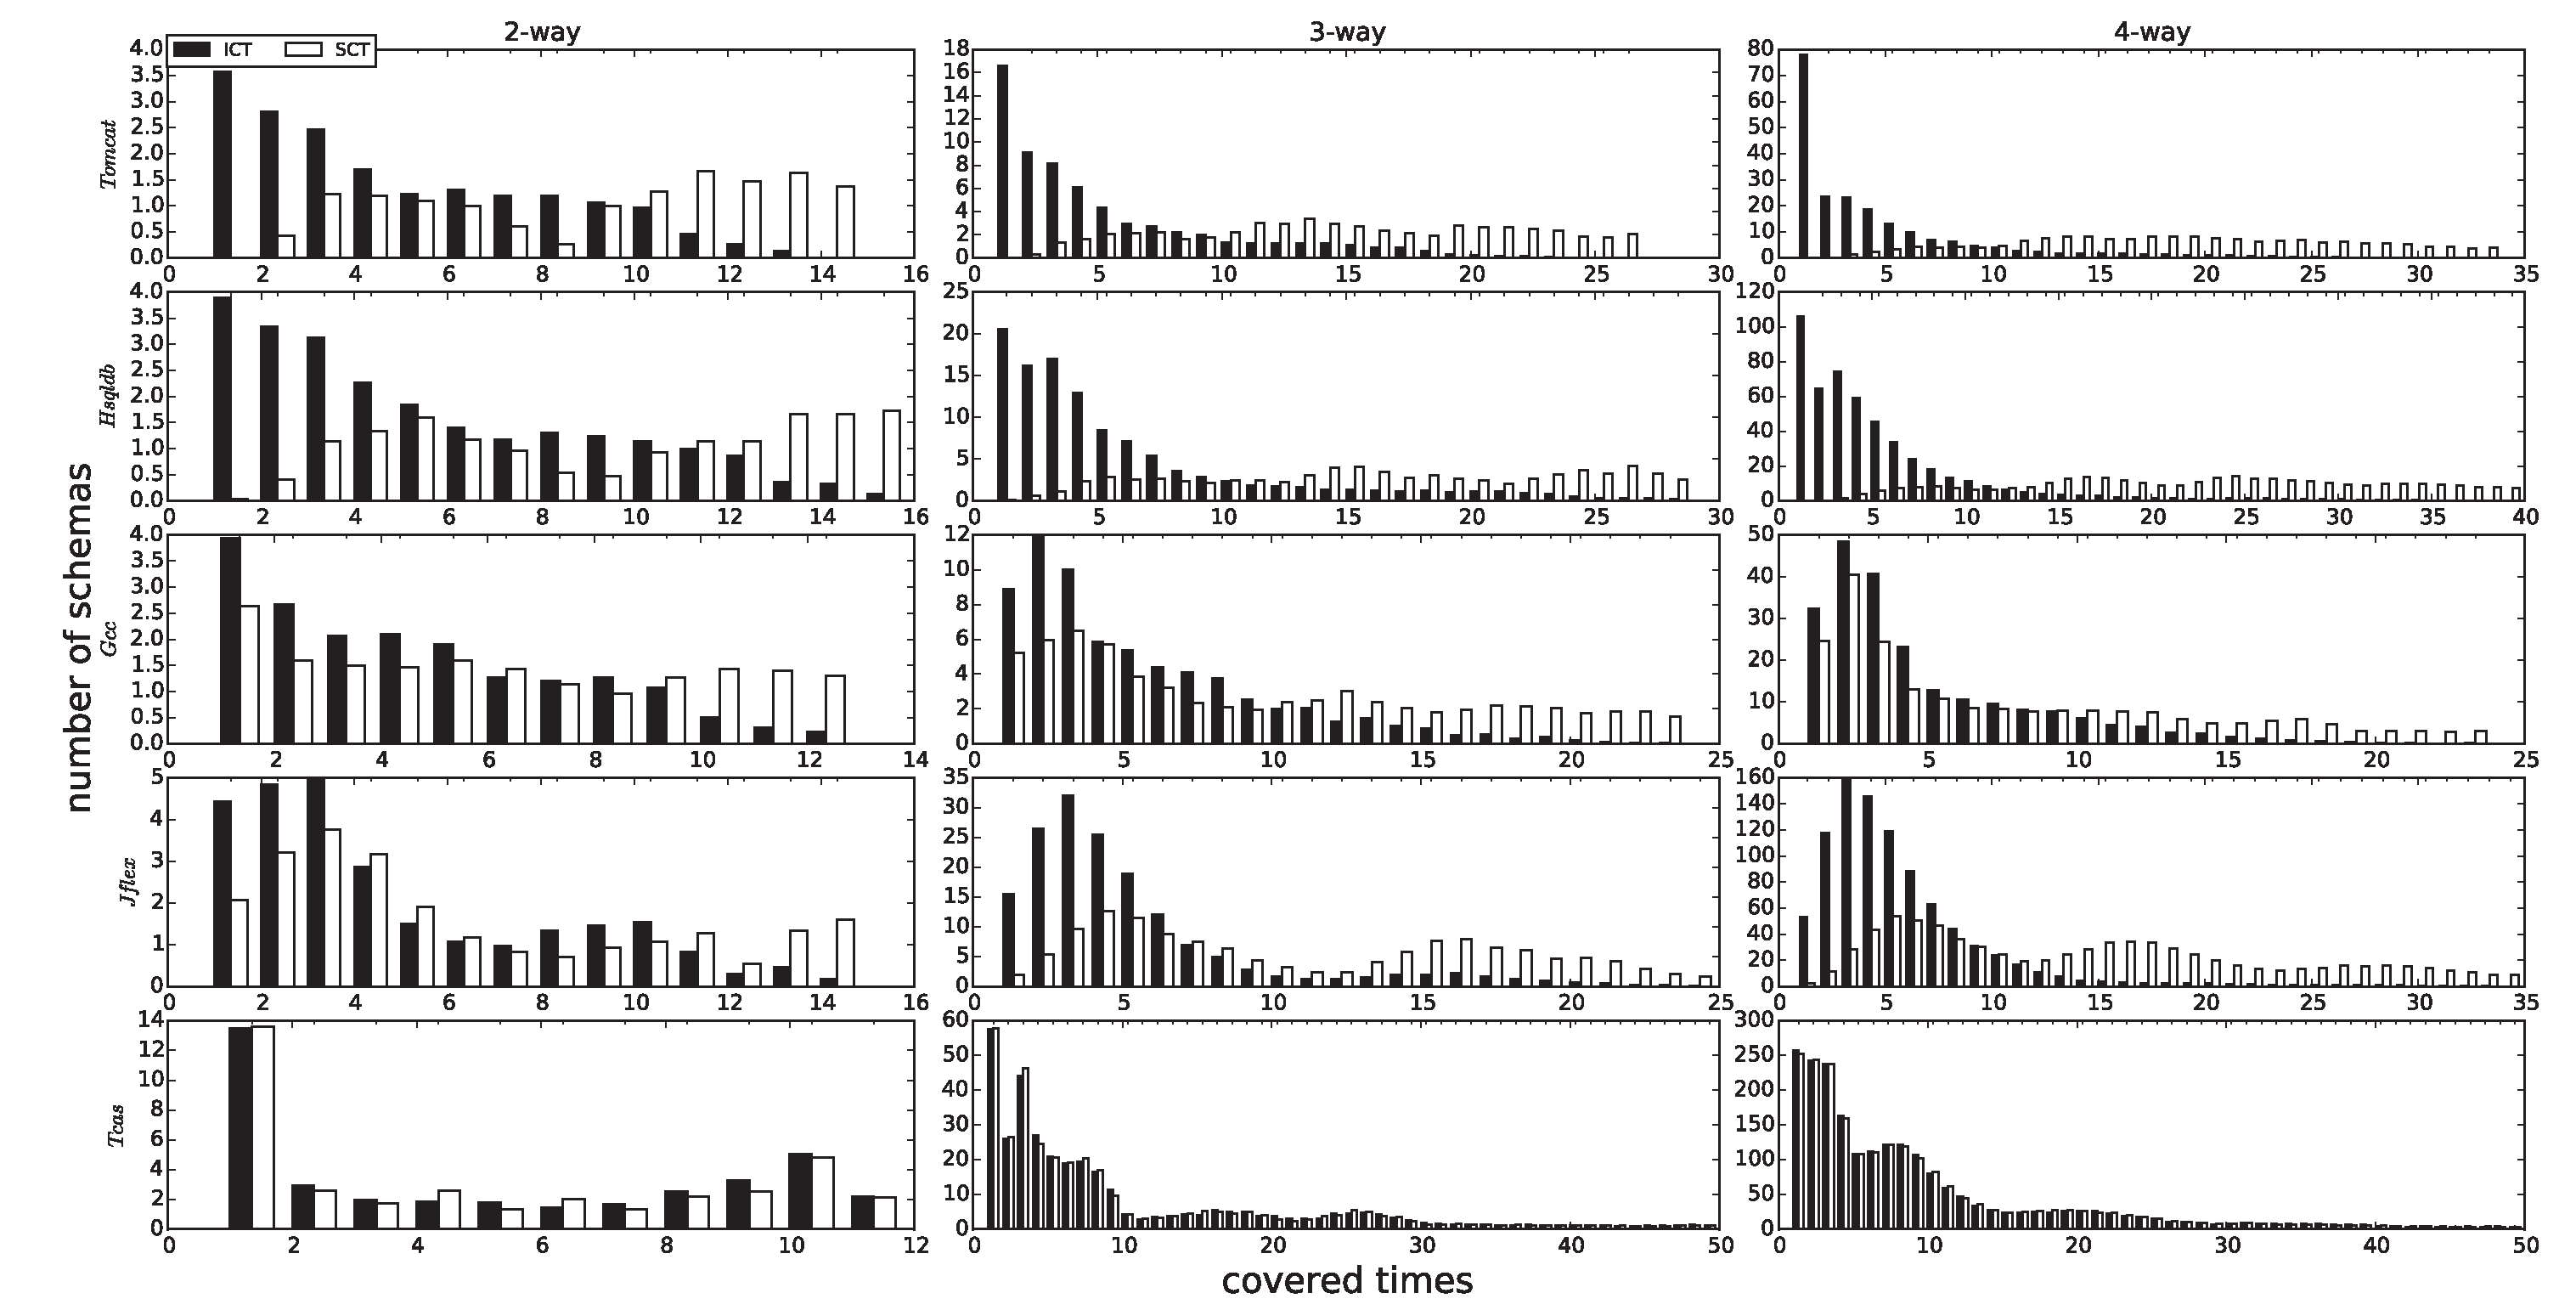
\includegraphics[width=7.0in]{ex1.eps}
\caption{The redundancy of test cases}
\label{ex1_result}
\end{figure*}

Our result is shown in Figure \ref{ex1_result}. This figure consists of 15 sub-figures, one for each subject with specific testing coverage (ranged from 2 - 4 way). For each sub-figure, the x-axis represents the number of times a schema is covered in total, and the y-axis represents the number of schemas.  For example in the first sub-figure (2-way for Tomcat), two bars with x-coordinate equal to 1 indicates that \emph{ict} approach had 61.5 schemas in average which were covered once and \emph{SCT} had 1.3 schemas.


As discussed previously, the more schemas are covered with a low-frequency, the less redundant the generated test cases are. Hence it implies an effective testing if the number of schemas (y-axis) decreases with the increase of the covered times (x-axis). With respect to Figure \ref{ex1_result}, it is easy to find that for most of the 15 sub-figures, \emph{ict} performed better than \emph{sct}. In fact, for \emph{ict}, the bars decreased rapidly with the increasing of the` x-axis, while for \emph{sct}, the trend was more smooth. See subject tomcat with 2-way coverage, for example, \emph{ict} had about 61.5 schemas which were only covered once,  about 38.9 schemas covered twice, less than 12 schemas covered more than 6 times.  For \emph{sct}, however, for most covered times, it had about 10 schemas, which indicates a very low performance.


%%%%%%%%%%%%%%%%%%%%%%%%%%%%%%%%%%%%%%%%%%%%%%%%%%%%%%%
The interesting exception is subject Tcas, on which \emph{ict} and \emph{sct} showed a similar trend. This is because all the MFS of Tcas are of high degree (t $>$ 6), and the covering arrays (t = 2, 3, 4) rarely detected any of them. Under this condition, since both approaches rarely detected the MFS, the overall process was transferred to be traditional covering array generation (the MFS identification process is omitted).

This result shows that our two modifications of the traditional approach, i.e., taking account of the covered schemas by test cases generated in MFS identification and forbidding the appearance of existing MFS to reduce the test cases that are used to identify the same MFS, are useful, especially when the MFS are detected and identified.

2) \textbf{Multiple MFS.}

The result is shown in Table \ref{multi_mfs}, which lists the number of test cases (on average for the repeated 30 experiments) that contain more than one MFS.

\begin{table}[ht]
\centering
\caption{Number of test cases that contain multiple MFS}
\label{multi_mfs}
\begin{tabular}{|ll|lll|}
\hline
Subject & Method & 2-way       & 3-way       & 4-way       \\ \hline
Tomcat	&ict	&0.0	&0.0	&0.0	\\
	&sct	&1.2	&4.6	&10.8	\\\hline
Hsqldb	&ict	&0.0	&0.0	&0.0	\\
	&sct	&0.2	&1.6	&4.1	\\\hline
Gcc	&ict	&0.5	&0.8	&0.6	\\
	&sct	&0.2	&1.8	&3.4	\\\hline
Jflex	&ict	&0.0	&0.0	&0.0	\\
	&sct	&0.0	&0.0	&0.0	\\\hline
Tcas	&ict	&0.0	&0.0	&0.0	\\
	&sct	&0.0	&0.0	&0.0	\\\hline
\end{tabular}
\end{table}



From this table, one observation is that \emph{ict} obtained a better result than \emph{sct} at limiting the test cases which contain multiple MFS. For all the subjects except \emph{Gcc}, \emph{ict} nearly eliminated all the test cases which contain multiple MFS. Even for \emph{Gcc}, the size of test cases which contain multiple MFS was limited in a very small number (smaller than 1). For \emph{sct}, however, the result was not as good as \emph{ict}. In fact, except for subjects \emph{Jflex} and \emph{Tcas}, \emph{sct} suffered from generating test cases which contain multiple MFS. This is one reason why even though \emph{sct} generated many more test cases than \emph{ict}, it did not obtain a better MFS identification result than \emph{ict}. Two exceptions are subjects \emph{Jflex} and \emph{Tcas}, on which both \emph{ict} and \emph{sct} did not generate test cases containing multiple MFS. The reason is that \emph{Jflex} has only one MFS (see Table \ref{inputs}) and the MFS of \emph{Tcas} are all high degrees which are hardly detected.


3) \textbf{Masking effects}.

\begin{table*}[ht]
\centering
\caption{Masking effects results}
\label{tested-t-way}
\begin{tabular}{|ll|lll|}
\hline
\multirow{2}{*}{Subjects} & \multirow{2}{*}{Method}& \multicolumn{3}{c|}{Tested-t-way coverage}      \\ \cline{3-5}
 &  & 2-way           & 3-way            & 4-way       \\ \hline
Tomcat	&ict	&\textbf{236.0}\textbf{(100.00\%)}	&\textbf{1424.0}\textbf{(100.00\%)}	&\textbf{5600.0}\textbf{(100.00\%)}	\\
	&sct	&233.8(99.07\%)	&1397.2(98.12\%)	&5501.7(98.24\%) 	\\\hline
Hsqldb	&ict	&\textbf{357.0}\textbf{(100.00\%)}	&\textbf{2742.0}\textbf{(100.00\%)}	&\textbf{14135.5}\textbf{(100.00\%)} \\
	&sct	&352.1(98.63\%)	&2713.7(98.97\%)	&13984.5(98.93\%) 	\\\hline
Gcc	&ict	&\textbf{251.4}\textbf{(99.76\%)}	&\textbf{1526.4}\textbf{(99.38\%)}	&\textbf{5997.6}\textbf{(99.17\%)} \\
	&sct	&250.0(99.21\%)	&1519.4(98.92\%)	&5908.2(97.69\%) 	\\\hline
Jflex	&ict	&\textbf{473.0}\textbf{(100.00\%)}	&\textbf{4282.0}\textbf{(100.00\%)}	&\textbf{26532.0}\textbf{(100.00\%)} \\
	&sct	&468.8(99.11\%)	&4216.6(98.47\%)	&26177.5(98.66\%)\\\hline
Tcas	&ict	&837.0(100.00\%)	&9158.0(100.00\%)	&64696.0(100.00\%) 	\\
	&sct	&837.0(100.00\%)	&9158.0(100.00\%)	&64696.0(100.00\%) \\\hline
\end{tabular}
\end{table*}



The results of masking effect for each approach is shown in Table \ref{tested-t-way}.  Specifically, the number of \emph{t}-degree (\emph{t} = 2, 3, 4) schemas which are \emph{tested} (in the passing test cases or identified as faulty schemas) are gathered, as well as the percentage of the total \emph{t}-degree schemas (in the parentheses followed).
%While the right part shows the number of test cases that ignores the masking effects (i.e., the test cases with no multiple MFS).
Several observations can be obtained from this result:


First, the extent to which \emph{sct} and \emph{ict} suffered from masking effects is not severe. Actually, the lowest tested-t-way coverage of \emph{ict} is 99.17\% (4-way for Gcc) and \emph{sct} is 97.69\% (4-way for Gcc). This result shows that combining MFS identification with covering array (either in the sequential way or interleaving way) can make testing more adequate than using covering array alone.
%Additionally, the number of test cases that ignores the masking effects accounts for a great proportion of the test cases in \emph{CT generation}, indicating that both approaches do not suffer too much from the masking effects.
% MFS identification into CT process, the is not very/ may be the subjects we handled are . If there are more than , may very .

%%%%%%%%------
Second, \emph{ict} was more effective than \emph{sct} at handling the masking effects. With respect to \emph{tested-t-way} coverage, \emph{ict} covered almost all the tested-t-way schemas for all the subjects (except for \emph{Gcc}, but for which \emph{ict} still covered more tested-t-way schemas than \emph{sct}). On the other hand, \emph{sct} was not as good as \emph{ict}. In fact, \emph{sct} fell behind \emph{ict} for almost all the subjects except \emph{Tcas}. For subject \emph{Tcas}, both \emph{ict} and \emph{sct} covered all the tested-t-way schemas (failures of \emph{Tcas} were rarely detected, and all the t-degree schemas appeared in the passing test cases).
%With respect to the test cases that were not masked by failures, we found the number of non-masked test cases generated by \emph{ict} was smaller than that of \emph{sct}, but this is mainly because the total number of test cases generated \emph{ict} was smaller than that of \emph{sct}. Based on these results, \emph{ict} is a better approach at avoiding the masking effects. We believe this is due to the higher quality of MFS identification of \emph{ict}, because it can better distinguish non-failure-inducing schemas from those MFS, and hence give those schemas more chances to be tested without the appearance of MFS.

%there are three cases that \emph{ict} are better than \emph{sct}, six cases that they are equal (for subjects \emph{Jflex} and \emph{Tcas}) and remaining six cases that \emph{sct} is better. With respect to the number of non-masked test cases,  the gap  between them is also trivial (no more than 10 test cases for all the 15 cases). As we discussed before, \emph{ict} forbids the appearance of identified MFS and can improve the performance at handling masking effects. The results, however, do not show this advantage. The reasons are manifold. Specifically, for \emph{ict}, while forbidding identified MFS in the later generated test cases can reduce masking effects, but the incorrectly identified MFS may make this effort in vain. That is, if the schemas identified by our framework is not the real MFS, then it will not contribute to the reduction on masking effects. This conclusion can also be manifested in Table \ref{cm_elda_fglt}, where the f-measure of ict is not always 1.0, indicating that the MFS identified is not always accurate. On the other hand, for \emph{sct}, while it does not forbid any MFS in the test case generation stage, but it generates more test cases than \emph{ict} (many of them are redundant and cover the same schemas several times). Hence, \emph{sct} may obtain more chances to revise their MFS identification. That is, if it incorrectly identifies the MFS in one failing test case, it may obtain the correct MFS in the next failing test case, and this will improve the performance on reduction of masking effects.

%One possible explanation for this is that \emph{sct} generates more test cases, of which some are passing test cases that cover more schemas.

%Third, if there is only single MFS or MFS is not detected, the tested-t-way coverage is 100\% for both \emph{ict} and \emph{sct}. This can be observed in subjects \emph{Jflex} and \emph{Tcas}, in which all the \emph{t}-degree schemas are covered. For single MFS, as MFS identification is effective, all the other \emph{t}-degree schemas can be determined as irrelevant to the failure. Consequently, the tested-t-way coverage is satisfied.  For the case that MFS cannot be detected (MFS with high degrees), traditional \emph{t}-way covering arrays are enough to obtain adequate testing, as all the test cases will pass if there is no MFS detected.

In summary, the answer to \textbf{Q2} is that \textbf{our approach \emph{ict} can alleviate the three problems discussed in Section \ref{sec:moti}, and when compared to \emph{sct}, \emph{ict} is a better approach to resolve these issues. Additionally, both \emph{ict} and \emph{sct} have a good performance on reducing the masking effects.}

\subsection{The benefits of feedback checking mechanism}
One important part of the \emph{ict} approach is the feedback checking mechanism, which aims at judging whether the schemas identified by \emph{ict} is real MFS or not by additionally generating test cases containing the schemas under check. It is interesting to evaluate how valuable is this feedback checking mechanism, i.e., how much improvement \emph{ict} gained from this mechanism.
%In this section, we need to find how benefits of our feedback checking schemas.
\subsubsection{Study setup}
For this, we created a mutation version of \emph{ict} by removing the feedback checking mechanism from the original \emph{ict} approach. We later call this mutation approach the \emph{ict-nonfb}.  Then, we applied this approach on testing the five subjects listed in Table \ref{subject} and identified the MFS contained in them. At last, we evaluated the benefits of the feedback checking mechanism by comparing the results obtained by \emph{ict-nonfb} and \emph{ict}.

%and the experiment as follows: ICT with feedback and ICT without feedback. And then show how they are work on the five experiments objects

\subsubsection{Result and discussion}
We list the results of the number of test cases generated by \emph{ict-nonfb} in Table \ref{tests-ict-nonfb}, the f-measure of MFS identification in Table \ref{fm-ict-nonfb}, the average number of test cases containing multiple MFS in Table \ref{multi-ict-nonfb}, and the tested-t-way coverage in Table \ref{tested-t-way-ict-nonfb}. Additionally, we attached the gaps between \emph{ict-nonfb} with ict in the parentheses. The value with a negative sign indicates the reduction in the corresponding metric (e.g., number of test cases, the f-measure, the number of test cases containing multiple MFS, the tested-t-way coverage) made by \emph{ict-nonfb} when compared with \emph{ict}, while non-negative sign indicates the increase in that corresponding metric.


\begin{table}[ht]
\caption{Number of test cases generated by \emph{ict} without feedback checking}
\label{tests-ict-nonfb}
\centering
    \begin{tabular}{|l|l|l|l|}
    \hline
 Subject      & 2-way                     & 3-way                     & 4-way                       \\ \hline
Tomcat	&42.8(-17.9)	&65.0(-14.9)	&115.2(-15.0)	\\
Hsqldb	&41.0(-8.4)	&74.2(-14.1)	&147.4(-18.9)	\\
Gcc	&37.0(-4.4)	&75.0(-14.0)	&121.4(-23.3)	\\
Jflex	&29.2(-2.4)	&63.2(-2.4)	&148.8(-1.9)	\\
Tcas	&111.0(\textbf{1.9})	&414.6(-3.1)	&1548.0(-4.8)	\\\hline
    \end{tabular}
\end{table}

\begin{table}[ht]
\caption{The f-measure obtained by \emph{ict} without feedback checking}
\label{fm-ict-nonfb}
\centering
    \begin{tabular}{|l|l|l|l|}
    \hline
 Subject      & 2-way                     & 3-way                     & 4-way                       \\ \hline
Tomcat	&1.0(0.00\%)	&1.0(0.00\%)	&1.0(0.00\%)	\\
Hsqldb	&0.74(-9.00\%)	&0.64(-36.00\%)	&0.64(-34.57\%)	\\
Gcc	&0.45(\textbf{10.95\%})	&0.46(-24.29\%)	&0.23(-55.71\%)	\\
Jflex	&1.0(0.00\%)	&1.0(0.00\%)	&1.0(0.00\%)	\\
Tcas	&0.0(0.00\%)	&0.0(0.00\%)	&0.01(0.00\%)	\\\hline
    \end{tabular}
\end{table}

\begin{table}[ht]
\caption{Number of test cases contain multiple MFS for \emph{ict} without feedback checking}
\label{multi-ict-nonfb}
\centering
    \begin{tabular}{|l|l|l|l|}
    \hline
 Subject      & 2-way                     & 3-way                     & 4-way                       \\ \hline
Tomcat	&0.0(0.0)	&0.0(0.0)	&0.0(0.0)	\\
Hsqldb	&0.0(0.0)	&0.0(0.0)	&0.0(0.0)	\\
Gcc	&0.4(-0.1)	&0.2(-0.6)	&1.2(\textbf{0.6})	\\
Jflex	&0.0(0.0)	&0.0(0.0)	&0.0(0.0)	\\
Tcas	&0.0(0.0)	&0.0(0.0)	&0.0(0.0)	\\\hline
    \end{tabular}
\end{table}

\begin{table}[ht]
\caption{The tested-t-way coverage obtained by \emph{ict} without feedback checking}
\label{tested-t-way-ict-nonfb}
\centering
    \begin{tabular}{|l|l|l|l|}
    \hline
 Subject      & 2-way                     & 3-way                     & 4-way                       \\ \hline
Tomcat	&236.0(0.00\%)	&1424.0(0.00\%)	&5600.0(0.00\%)	\\
Hsqldb	&356.8(-0.06\%)	&2729.4(-0.46\%)	&14026.8(-0.77\%)	\\
Gcc	&251.2(-0.08\%)	&1485.6(-2.67\%)	&5701.2(-4.94\%)	\\
Jflex	&473.0(0.00\%)	&4282.0(0.00\%)	&26532.0(0.00\%)	\\
Tcas	&837.0(0.00\%)	&9158.0(0.00\%)	&64696.0(0.00\%)	\\\hline
    \end{tabular}
\end{table}

The following could be observed:

1) \emph{ict-nonfb} generated a smaller amount of test cases than \emph{ict}. Specifically, except for the \emph{tcas} program subject, \emph{ict-nonfb} reduced ranged from 1.9 to 23.3 number of test cases. This is as expected because the feedback checking mechanism needs to generate additional test cases to check whether the schemas identified by \emph{ict} is real MFS or not.

2) The quality of the MFS identification of \emph{ict-nonfb} decreased a lot. In fact, except for the 2-way coverage of \emph{Gcc}, \emph{ict} either obtained higher f-measures or performed equally well on all the remaining subjects of all the t-ways (2, 3, and 4-way coverage). Additionally, the gaps between them ranged from 9\% to 55.7\%, which is not trivial.


3) There were no distinct gaps between \emph{ict-nonfb} and \emph{ict} at the number of test cases that containing multiple MFS. In fact, for all the subjects except for \emph{Gcc}, \emph{ict-nonfb} and \emph{ict} both generated 0 test case that containing multiple MFS. For \emph{Gcc}, \emph{ict-nonfb} performed better at 2-way (but the gap is only 0.1) and 3-way coverage, while \emph{ict} performed better at 4-way coverage.
%However, considering that \emph{ict} generated more test cases than \emph{ict-nonfb}, ict seemed get a better limiation.

4) The tested-t-way coverage of \emph{ict-nonfb} also decreased. In fact, besides those subjects that \emph{ict-nonfb} and \emph{ict} performed equally well, \emph{ict-nonfb} reduced the tested-t-way coverage by about ranged from 0.02\% (0.2 tested-2-way schemas) to 4.94\% (296.4 tested-4-way schemas).

To summarize, the answer to \textbf{Q3} is that:
\textbf{Without feedback  checking mechanism, the number of test cases generated by \emph{ict} reduced, but the quality of MFS identification and tested-t-way coverage decreased significantly. It indicates that the additional test cases generated in feedback  checking mechanism is worthwhile, and it is beneficial to adopt feedback checking mechanism in the CT process (in order to obtain a better MFS identification result and a higher tested-t-way coverage).
}
%


\subsection{Comparison with FDA-CIT}\label{sec:emprical:CompareFDA}
\begin{figure}[ht]
 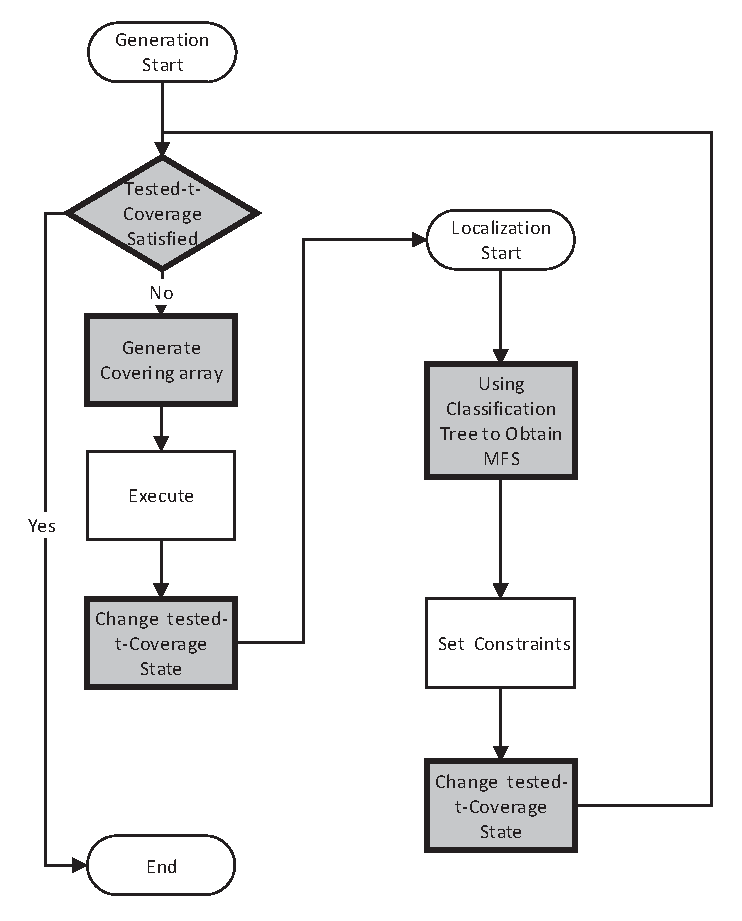
\includegraphics[width=3.4in]{fd-cit.eps}
\caption{The Framework of fda-cit}
\label{fda-cit-life}
\end{figure}
\emph{fda-cit} \cite{yilmaz2013reducing} is a feedback framework that can augment the traditional covering array to iteratively identify the MFS and can handle the masking effects. The overall process can be illustrated in Figure \ref{fda-cit-life}. Specifically, it will first generate a \emph{t}-way covering array and execute all the test cases in it. After that it will utilize the classification tree method to identify the MFS. Then it will forbid the identified MFS to appear and compute the tested-t-way coverage. If the tested-t-way coverage is not satisfied, it will repeat the previous process, i.e., generating additional test cases and identifying MFS. Like our \emph{ict} approach, FDA-CIT is also an adaptive approach which iteratively generates test cases and identifies the MFS. Besides these commonalities, there are several important differences between our approach and \emph{fda-cit} (shaded in Figure \ref{fda-cit-life}):

First, the \textbf{granularity} of adaptation. Instead of handling one test case one time as \emph{ict}, \emph{fda-cit} tries to generate a batch of test cases at each iteration (A complete covering array will be generated at the first iteration, and more test cases will be supplemented to cover those \emph{t}-degree schemas which are masked at the following iterations). To generate a batch of test cases may improve the degree of parallelism of testing, but this coarser granularity may also introduce some problems, e.g., some test cases generated at one iteration may fail with the same MFS, which is a potential waste because it is better to use one failing test case to reveal one particular MFS.

Second, the \textbf{MFS identification} approach is different. \emph{fda-cit} uses the classification tree on existing executed test cases to characterize the MFS. Different from our OFOT approach, this post-analysis technique does not need additional test cases, but as a side effect it cannot precisely find the MFS. Worse, the effectiveness of this post-analysis approach depends greatly on the covering array, e.g., if there are a large number of failing tests, and a small size test suite, there is little information to exclude the particular MFS \cite{zhang2011characterizing}.

Third, the \textbf{coverage criterion} is not the same. \emph{fda-cit} directly uses the tested-t-way coverage to guide their process. This supports a better adequate testing and reduces the impacts of masking effects. As we will see later in our experiments, however, the incorrect MFS identification may prevent \emph{fda-cit} from reaching this type of coverage.

%Next, we will design experiments to measure the performance of \emph{fda-cit}.

\subsubsection{Study setup}
The design of this case study is similar to the previous two. For each subject in Table \ref{subject}, we applied \emph{fda-cit} to generate test cases and identify the MFS. After that, we gathered the overall test cases generated (\emph{fda-cit} does not need additional test cases to identify the MFS), MFS identification results(including recall, precision and f-measure), and the other three metrics, i.e., covered times of schemas, the number test cases which contain multiple MFS, and the tested-t-coverage. The same as previous experiments, we repeated each experiment 30 times for different coverage (2, 3, and 4 way), and then gathered and analysed the average data.  Note that the MFS identification approach in the \emph{fda-cit} has two versions, i.e., ternary-class and multiple-class. In this paper, we use the multiple-class version for comparison, as it performs better than the former \cite{yilmaz2013reducing}. Another point needs to be noted is that we also used the augmenting simulated annealing approach \cite{cohen2003augmenting,cohen2008constructing2} to build covering array for the \emph{FDA-CIT}.

%Note that in this study, we do not gather the test cases which contain multiple MFS, as the post-analysis classification tree method is not affected by this factor.

\subsubsection{Result and discussion}

1) \textbf{Total number of test cases}
The total number of test cases generated by \emph{fda-cit} for each subject is shown in Table \ref{num-fda-cit}. To better evaluate the performance of \emph{fda-cit}, we list the gaps between FDA-CIT with ict and sct respectively in the parentheses (the first number is for \emph{ict}, the second one is \emph{sct}). The value with a negative sign indicates the reduction in the test cases between \emph{fda-cit} and other two approaches, while the value without negative sign indicates the number of test cases which \emph{fda-cit} generated more than the other two approaches.

\begin{table*}[ht]
\caption{Number of test cases generated by \emph{fda-cit}}
\label{num-fda-cit}
\centering
    \begin{tabular}{|l|l|l|l|}
    \hline
    ~      & 2-way                     & 3-way                     & 4-way                       \\ \hline
Tomcat	&28.4(-32.3,-39.9)	&65.5(-14.4,-34.2)	&147.4(\textbf{17.2},-39.9)	\\
Hsqldb	&29.9(-19.5,-18.0)	&83.5(-4.8,-29.8)	&201.2(\textbf{34.9},-35.3)	\\
Gcc	&21.7(-19.7,-12.7)	&63.4(-25.6,-16.8)	&120.7(-24.0,-19.4)	\\
Jflex	&19.8(-11.8,-12.7)	&64.5(-1.1,-9.5)	&179.5(\textbf{28.8},\textbf{1.8})	\\
Tcas	&109.9(\textbf{0.8},\textbf{2.4})	&416.6(-1.1,-1.7)	&1544.7(-8.1,-14.0)	\\\hline
    \end{tabular}
\end{table*}

From this table, one observation is that \emph{fda-cit} was better than \emph{sct} at almost all cases. Combining the results of previous studies for \emph{sct} and \emph{ict}, we can conclude that \emph{sct} was the most inefficient approach at test case generation. Second, for \emph{ict} and \emph{fda-cit}, there were ups and downs on both sides. In detail, \emph{fda-cit} needed fewer test cases at lower coverage (2-way  and 3-way coverage), while \emph{ict} performed better at higher coverage (4-way).

This result is reasonable. First, \emph{fda-cit} did not need additional test cases to identify the MFS, which would reduce some cost when compared with \emph{ict}, especially when the coverage is low (For low coverage, the test cases generated by \emph{ict} in the MFS identification stage account for a considerable proportion of the overall test cases). On the other hand, as noted earlier, the coarse-grained generation would make fda-cit generate some unnecessary test cases.

2) \textbf{F-measure of MFS identification} The results of the quality of MFS identification by \emph{fda-cit} is listed in Table \ref{f-measure-fda-cit}. Same as the previous metric, the comparison between fda-cit with \emph{ict} and \emph{sct} is also attached (the first number is for \emph{ict}, the second one is \emph{sct}).

\begin{table*}[ht]
\caption{The F-measure of MFS identification for \emph{fda-cit}}
\label{f-measure-fda-cit}
\centering
    \begin{tabular}{|l|l|l|l|}
    \hline
           & 2-way                   & 3-way                   & 4-way                   \\ \hline
Tomcat	&0.22(-77.57\%,-63.28\%)	&0.31(-69.09\%,-61.94\%)	&0.33(-66.67\%,-59.52\%)	\\
Hsqldb	&0.32(-51.26\%,-18.26\%)	&0.29(-71.12\%,-20.45\%)	&0.32(-66.19\%,-10.76\%)	\\
Gcc	&0.07(-26.48\%,-2.19\%)	&0.4(-30.28\%,\textbf{31.50\%})	&0.49(-29.57\%,\textbf{38.29\%})	\\
Jflex	&1.0(0.00\%,0.00\%)	&1.0(0.00\%,0.00\%)	&1.0(0.00\%,0.00\%)	\\
Tcas	&0.0(0.00\%,0.00\%)	&0.0(0.00\%,0.00\%)	&0.0(-0.81\%,0.00\%)	\\\hline
    \end{tabular}
\end{table*}

This table shows a discernible disparity between \emph{fda-cit} with the other two approaches. In fact, besides subject \emph{Jflex} of which all three approaches accurately identified the single low-degree MFS (with F-measure equal to 1), and subject \emph{Tcas} of which all three approaches could hardly detect failures (with F-measure equal to 0), \emph{ict} led over \emph{fda-cit} by about 26\% to 77\%, which is not trivial. The result is similar when comparing \emph{sct} with \emph{fda-cit}.

%Another interesting observation is for subject \emph{Tcas}, which has multiple high degree MFS. We can find that, although very trivial, \emph{sct}  and \emph{ict} have identified some high-degree MFS (F-measures of 3-way and 4-way is not equal to 0). However, fda-cit failed to accurately identify even one high-degree MFS, as all f-measure equal to 0.

This result suggests that the classification tree approach used by \emph{fda-cit}, although very resource-saving (does not need additional test cases),  is ineffective to accurately identify MFS, especially when there are multiple MFS with high degrees.

Note that \emph{fda-cit}'s primary concern is to avoid masking effects and to give every $t$-degree schema a fair chance to be tested, not to perform fault characterization. On the other hand for the classification tree method, when only a very small set of test cases fail, it will result in the input data for classification tree to be highly unbalanced \cite{zhang2012faulty}. Another point is that all the MFS identified by the classification tree method should contain the same parameter value on the root, which will result in the schemas identified by \emph{fda-cit} tending to be super-schema of the real MFS.
%Although this leads to the f-measure of MFS identification lower than that of \emph{ict}, it does not have much negative influence on the masking effects reduction. This is because to forbid the appearance of super-schema of real MFS will not reduce the number of schemas that is not MFS to be tested. As a result, the \emph{tested-t-way} coverage is not changed (This coincides well with the experimental results).

3) \textbf{Redundant test cases}.
The result is listed in Figure \ref{ex2_result}. The same as Figure \ref{ex1_result}, for each sub-figure, the x-axis represents the number of times a schema is covered in total, and the y-axis represents the number of schemas.  To enable an intuitive comparison with \emph{ict} and \emph{sct}, we attach the data for \emph{ict} and \emph{ict}, with solid line and dotted line, respectively.

\begin{figure*}[htbp]
 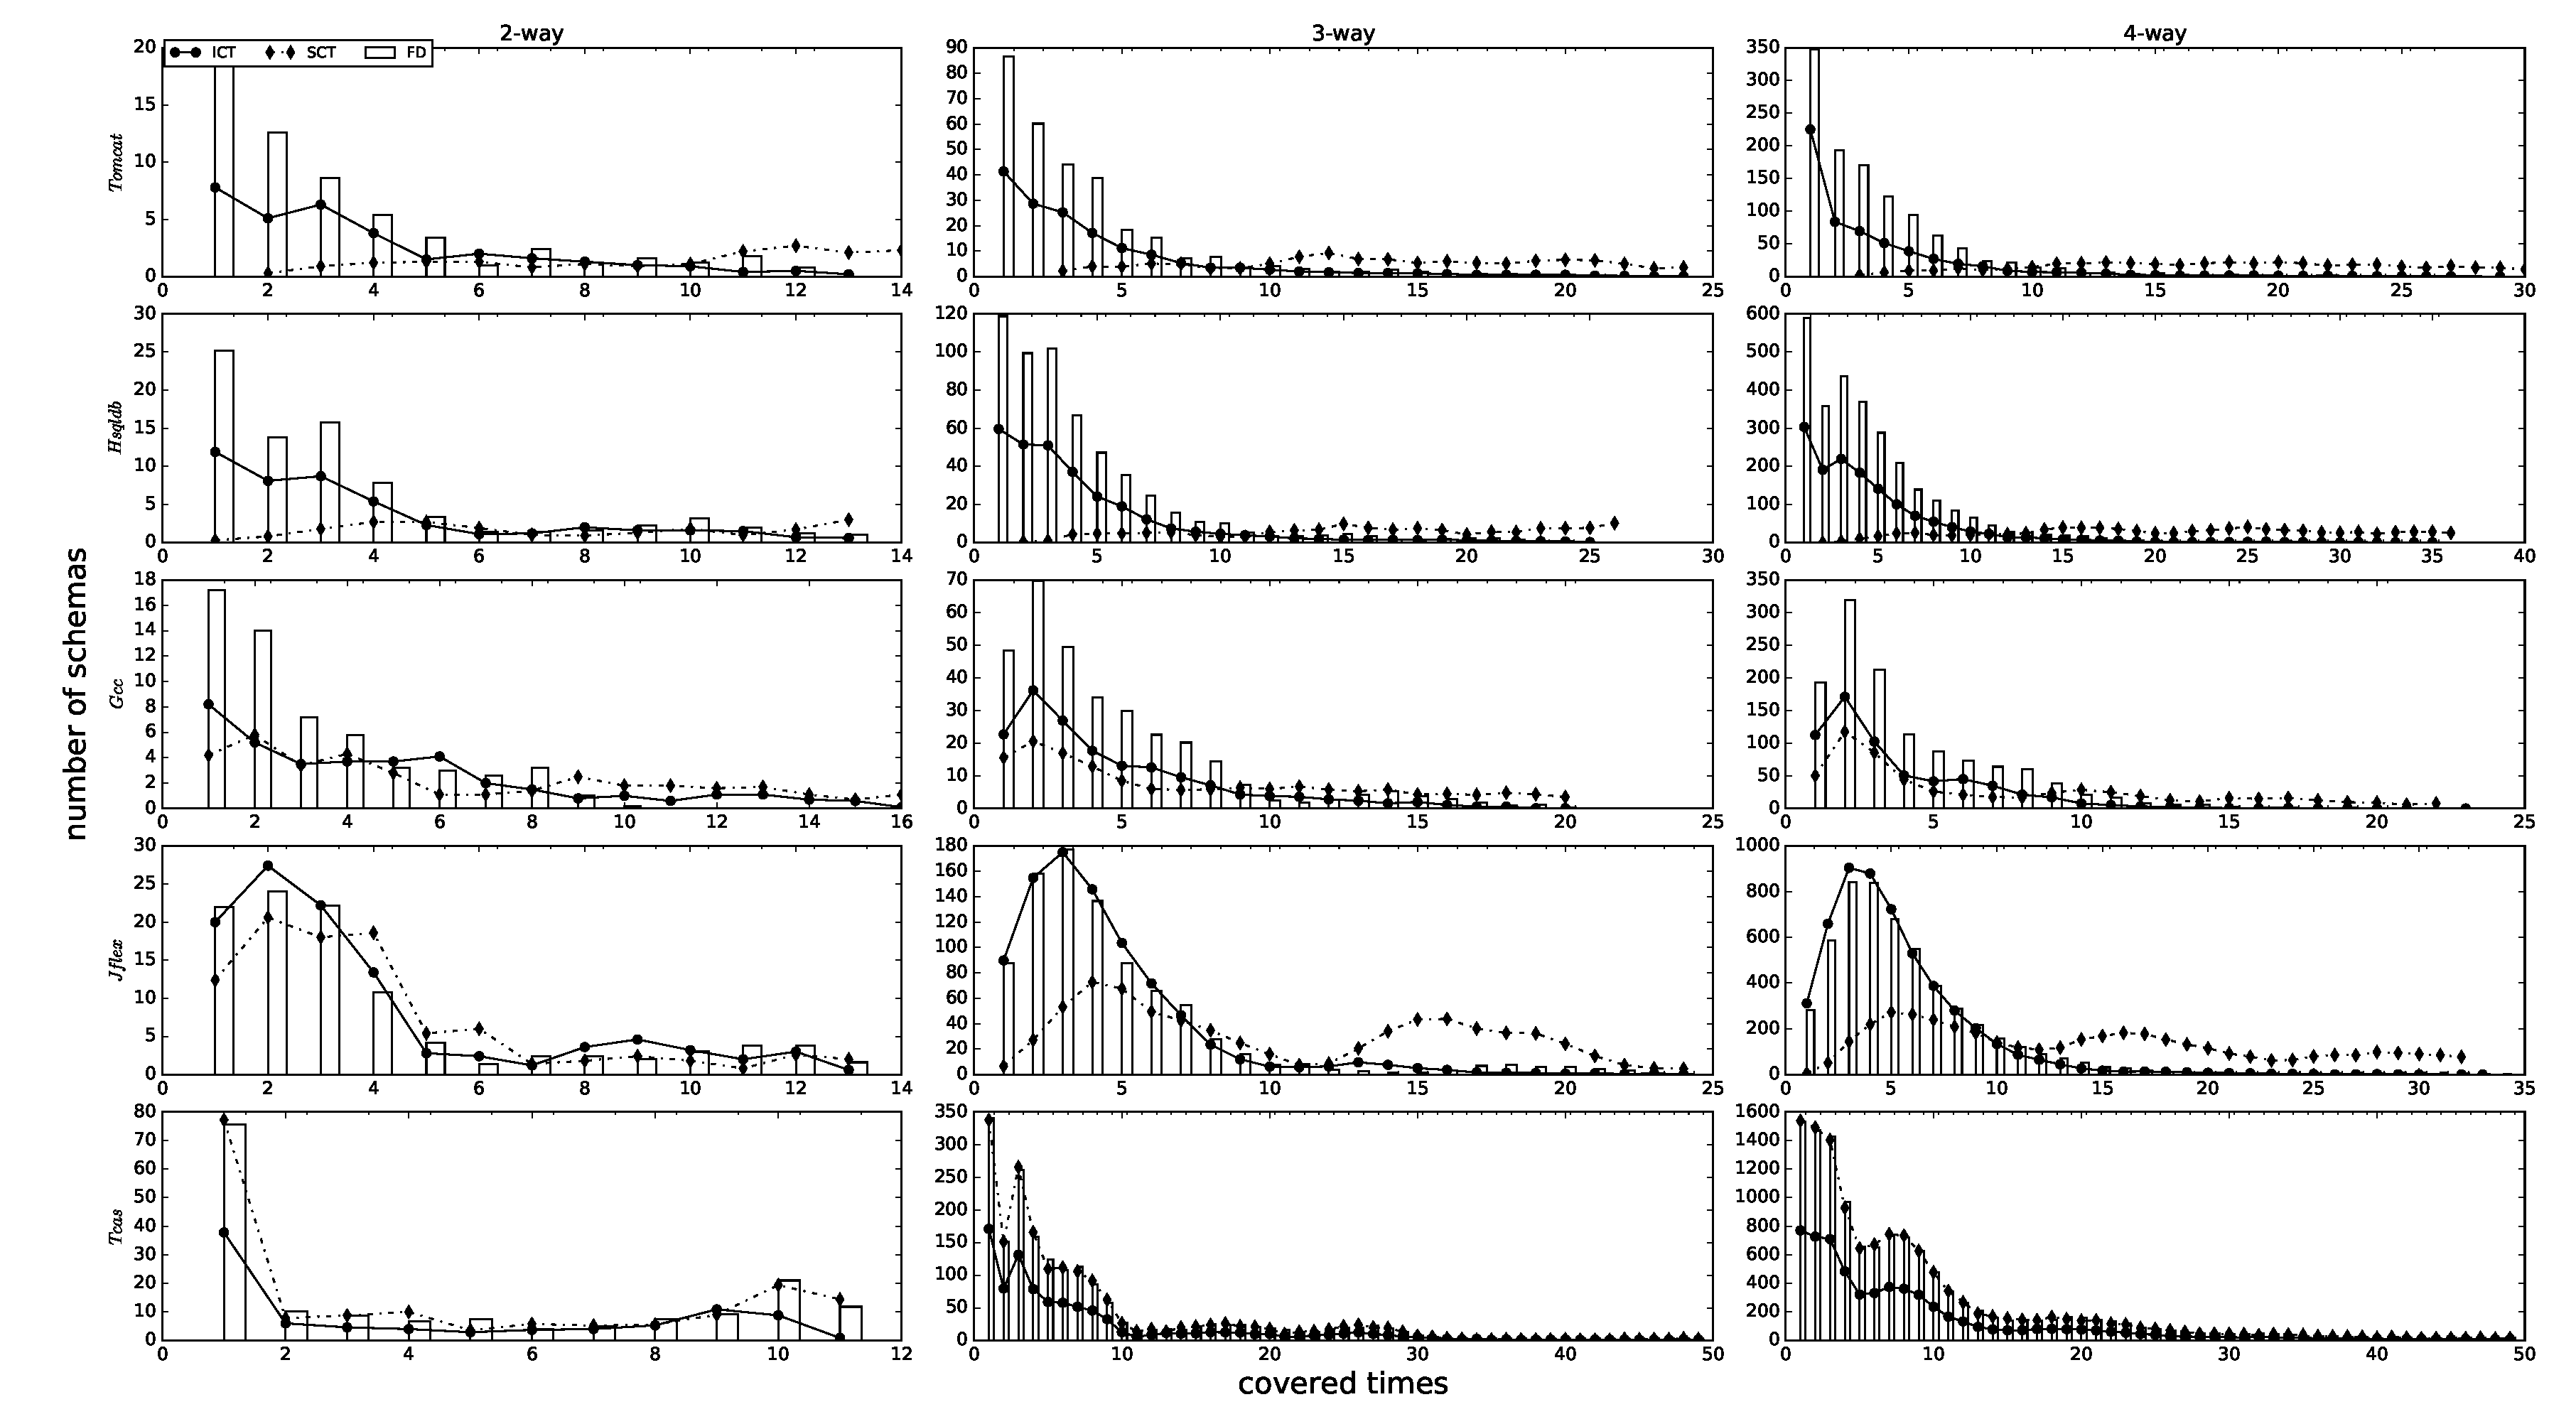
\includegraphics[width=7.0in]{ex2.eps}
\caption{The redundancy of test cases generated by \emph{fda-cit}}
\label{ex2_result}
\end{figure*}

From this figure, we can see the trend of the bars of \emph{fda-cit} matches pretty well with the curve representing \emph{ict}, which has a significant advantage over the curve of \emph{sct}. This result implies that the test case redundancy of \emph{ict} is similar to that of \emph{fda-cit}, which is not severe when compared with \emph{sct}.

%i.e result implies that the test case redundancy between \emph{ict} and \emph{fda-cit} are similar, which is not severe when comparing with \emph{sct}.

4)\textbf{Test Cases containing multiple MFS}

Table \ref{multi-fda-cit} shows the number of test cases that contain multiple MFS on average for \emph{fda-cit}. The same as before, we also list the gaps between \emph{fda-cit} with \emph{ict} and \emph{sct} respectively in the parentheses (the first number is for \emph{ict}, the second one is for \emph{sct}). From this table, we can easily find that \emph{fda-cit} did almost the same as \emph{sct} at restricting the appearance of test cases that contain multiple MFS. But both of them did not as well as \emph{ict}. In fact, except for subject \emph{Jflex} (which contains single MFS) and \emph{Tcas} (which contains high-degree MFS that are rarely detected), \emph{fda-cit} generated more test cases that contain multiple MFS than \emph{ict}, and the gap between them increased with the increasing of test coverage (\emph{fda-cit} generated about 1 more test cases for 2-way coverage, 2 more test cases for 3-way coverage, and 5 more test cases for 4-way coverage). This result shows that \emph{ict} was the best approach among them to reduce the appearance of test cases that contain multiple MFS, and we also believe this is one reason why \emph{ict} obtained a higher-quality of MFS identification.

%%%%%%%%%%%%%%%%%%%%%%%%%%%%%%%%%%%%%%%%%%%%%%%%%%%%%%%%%%%%%%%%%%%%%%%%%%%%%%%%%------%%%%%%%%%%%%%%%%%%%%%%

\begin{table}[ht]
\caption{Number of test cases contain multiple MFS for \emph{fda-cit}}
\label{multi-fda-cit}
\centering
    \begin{tabular}{|l|l|l|l|}
    \hline
                   & 2-way                    & 3-way                      & 4-way                       \\ \hline
Tomcat	&0.9(\textbf{0.9},-0.3)	&4.5(\textbf{4.5},-0.1)	&9.8(\textbf{9.8},-1.0)	\\
Hsqldb	&0.4(\textbf{0.4},\textbf{0.2})	&1.5(\textbf{1.5},-0.1)	&4.9(\textbf{4.9},\textbf{0.8})	\\
Gcc	&2.4(\textbf{1.9},\textbf{2.2})	&2.5(\textbf{1.7},\textbf{0.7})	&4.1(\textbf{3.5},\textbf{0.7})	\\
Jflex	&0.0(0.0,0.0)	&0.0(0.0,0.0)	&0.0(0.0,0.0)	\\
Tcas	&0.0(0.0,0.0)	&0.0(0.0,0.0)	&0.0(0.0,0.0)	\\\hline
    \end{tabular}
\end{table}


5)\textbf{Masking effects}.
%and Table \ref{non-mask-fda-cit}
The result is listed in Table \ref{tested-t-coverage-fda-cit}, which shows the results of \emph{tested-t-way} coverage. The gaps between \emph{fda-cit} with \emph{ict} and \emph{sct} are listed in the parentheses, respectively (the first one is \emph{ict}, the second one is \emph{sct}).

With regard to \emph{tested-t-way} coverage, we can find that our approach \emph{ict} was still the best approach at reducing the masking effects, even though when compared with approach \emph{fda-cit}. In fact, among the 15 cases listed in Table \ref{tested-t-coverage-fda-cit}, there are 13 cases on which \emph{ict} performed equal to or better than \emph{fda-cit} (The only two exceptions are \emph{Gcc} for 3-way and 4-way coverage). Note that on some particular cases, the gaps between \emph{ict} and \emph{fda-cit} are not trivial, e.g., \emph{ict} obtained 10 more percent of tested-t-way coverage than \emph{fda-cit} at 2-way coverage for subject \emph{Tomcat}).

%For example, \emph{fda-cit} decreased about 5.71\%  and 7.61\% at tested-2-way coverage than \emph{ict} and \emph{sct}, respectively,  for the subject Tomcat, but also increased about 1.68\% at tested-3-way coverage than \emph{ict} for subject Tomcat, and is about 0.18\% better than \emph{sct} at tested-4-way coverage for subject Hsqldb. In fact, there are three cases (shown in bold) that \emph{fda-cit} performed better than \emph{ict}, and six cases that \emph{fda-cit} did not. The gap between the three approaches for \emph{tested-t-way} coverage is very trivial.

%--------------------------------------------


%With regard to \emph{the number of test cases which ignore the masking effects}, we find that for almost all the cases (except for tested-3-way coverage of Tcas), \emph{fda-cit} performed better than both \emph{ict} and \emph{sct}. This is because for approaches \emph{ict} and \emph{sct}, the proportion of test cases for identifying the MFS is not trivial, and the test cases that aim to identify MFS are more likely to be affected by masking effects (many of them will contain the MFS and fail during testing). Considering there is little difference between the overall size of test cases generated by \emph{fda-cit} and \emph{ict}, it is easy to learn that the number of test cases generated for \emph{CT generation} of \emph{fda-cit} is larger than that of \emph{ict} and \emph{sct}. As a consequence, the number of test cases generated by \emph{ict} that can be counted as ignoring the masking effects is smaller than that of \emph{fda-cit}. However, if we consider the proportion of the test cases for \emph{CT generation}, these two approaches actually performed similarly at \emph{the number of test cases which ignore the masking effects}.
%Specifically, there
%In other words, if we take the test cases for identifying the MFS into account for \emph{ict}, \emph{the number of test cases which ignore the masking effects} of \emph{ict} is actually similar to that of \emph{fda-cit}.

%they need to generate test cases for identifying the MFS. These test cases, however, very likely contain multiple MFS (they are ).

Above all, this result suggests that our approach \emph{ict} does reach the same or better level when compared with \emph{fda-cit} at reducing the masking effects. The conclusion also implies that, to limit the masking effects, only using an adaptive framework to separately identify the MFS is not enough; making MFS identification accurate is more important.

\begin{table*}[ht]
\caption{The tested-t-way coverage for \emph{fda-cit}}
\label{tested-t-coverage-fda-cit}
\centering
    \begin{tabular}{|l|l|l|l|}
    \hline
           & 2-way                    & 3-way                      & 4-way                       \\ \hline
Tomcat	&212.1(-10.13\%,-9.28\%)	&1390.2(-2.37\%,-0.50\%)	&5378.0(-3.96\%,-2.25\%)	\\
Hsqldb	&345.1(-3.33\%,-1.99\%)	&2725.1(-0.62\%,0.42\%)	&14096.7(-0.27\%,0.80\%)	\\
Gcc	&250.2(-0.48\%, 0.08\%)	&1530.8(0.29\%,0.74\%)	&6017.5(0.33\%,1.82\%)	\\
Jflex	&473.0(0.00\%,0.89\%)	&4282.0(0.00\%,1.53\%)	&26532.0(0.00\%,1.34\%)	\\
Tcas	&837.0(0.00\%,0.00\%)	&9158.0(0.00\%,0.00\%)	&64695.9(-0.00\%,-0.00\%)	\\\hline
    \end{tabular}
\end{table*}

%\begin{table*}[ht]
%\caption{Non-masked test cases for \emph{fda-cit}}
%\label{non-mask-fda-cit}
%\centering
%    \begin{tabular}{|l|l|l|l|}
%    \hline
%               & 2-way                    & 3-way                      & 4-way                       \\ \hline
%Tomcat	&27.5(19.2,14.9)	&61.0(29.9,26.7)	&137.6(58.7,55.6)	\\
%Hsqldb	&29.5(17.8,14.1)	&82.0(41.3,35.2)	&196.3(83.3,77.4)	\\
%Gcc	&19.3(5.8,4.9)	&60.9(20.1,9.8)	&116.6(22.9,18.1)	\\
%Jflex	&19.8(5.2,3.9)	&64.5(15.9,14.6)	&179.5(45.8,46.3)	\\
%Tcas	&109.9(0.8,2.4)	&416.6(1.9,\textbf{-1.7})	&1544.7(\textbf{-0.7},\textbf{-11.4})	\\\hline
%    \end{tabular}
%\end{table*}


To summarize, the answer to \textbf{Q4} is that
\textbf{when compared to the adaptive CT approach \emph{fda-cit}, our approach \emph{ict} performed more effectively, especially at the quality of MFS identification and reduction of masking effects, while there are no apparent differences between them at the cost (the number of test cases). This also indicates that \emph{ict} is a more efficient approach.}
%Additionally, our approach supports a better MFS identification than \emph{fda-cit}.


Note that one reason that \emph{ict} did not generate more test cases than \emph{fda-cit} is that all the subjects we used in the experiments have just one test file for each test configuration. Here test configuration equals to the test case we discussed throughout the paper.    \emph{fda-cit} is designed to work better for subjects of which one configuration has multiple test files. Under the scenario of multiple test files, \emph{cit} should separately handle each of them, because each test file may contain distinct MFS. As a result, the number of additional configurations needed will grow linearly with the number of failing test files. Under this case, \emph{fda-cit} needs a smaller amount of test cases \cite{yilmaz2013reducing}.

%    especially on reducing the redundancy of test cases and limiting the test cases with multiple MFS. Additionally, both \emph{ict} and \emph{sct} have a good performance on reducing the masking effects.

%\subsection{Combination of two approaches}
%To combine two approaches . However, not all combination is good. For example, if two approaches get the similar results. The combination of them does not improve the result, but will cost more as we does two approaches, indicating more test cases are generated. Hence, we needs to the results of two approaches as difference as possible. The ideal scenario, is , one MFS cannot be identified by this approach, but can identified by another approach.
%
%\subsubsection{Study setup}
%We count each MFS identified by each approach. To count the . To measure the difference of two approaches, we introduce the ratio . that is . the.  which are .
%
%The more the . the more difference are , and indicating the better the complementary of two approaches (������). 2Latter we will compare the complentary from the combination of ICT and SCT with  the combination of ICT and \emph{fda-cit}.
%
%
%\subsubsection{Result and discussion}
%


%  comparing there are two shortcomings for the traditional, first, it needed much more test cases that ours, second, it has an lower quality of the identified MFS .
%\subsection{Compare with the \emph{fda-cit}}
%
%\subsubsection{Study setup}
%
%
%\subsubsection{Result and discussion}


\subsection{Multiple defects}
Since there is only one defect in each software subject used in the previous experiments, it is interesting to observe how well these approaches work on programs with multiple defects. To identify the MFS in the programs with multiple defects is more complex than in the software with a single defect. One problem is that one defect may crash the system under test so that other defects will not have the chance to be triggered. Even worse, some defects may have interference between each other \cite{wong2016survey}, e.g., constructive and destructive interference \cite{debroy2009insights}, making fault localization more difficult.  For all these reasons, it is important to conduct experiments on multiple defects.
%we adopt the following rules, distingusging failures.

\subsubsection{Study setup}
The software subjects with multiple bugs used in this experiment are listed in Table \ref{multiple_defects_subjects}. In this table, we listed corresponding versions of each software, lines of code, number of classes, the bug IDs, their corresponding input model, and MFS information.

\begin{table*}[ht]
\caption{The software subjects with multiple defects}
\label{multiple_defects_subjects}
\centering
\begin{tabular}{|c|c|c|c|c|c|c|} \hline
Software&  Version & Loc & Classes & Bug \# & Input Model & MFS\\ \hline

Hsqldb& 2.0rc8 & 139425 & 495 &  \#981 \& \#1005 & $2^{9}\times 3^{2} \times 4^{1}$ & 3(5)\\
	  &2.2.5 & 156066 & 508 & \#1173 \&  \#1179 & $2^{8} \times 3^{3}$ & 2(1)\ 1(1)\\
	    &2.2.9 & 162784 &525 & \#1286 \& \#1280 & $2^{8} \times 3^{3}$ & 3(2)\ 2(1)\ 1(1)\\ \hline
Jflex& 1.4.1 &  10040 &58 & \#87 \& \#80  & $2^{10} \times 3^{2} \times 4^{1}$ & 1(2)\\
    &  1.4.2 &  10745 &61 &  \#98 \& \#93 & $2^{11} \times 3^{2} \times 4^{1}$ & 2(1)\ 1(1)\\ \hline
\end{tabular}
\end{table*}

For each subject, we applied the previous three approaches, i.e., \emph{ict}, \emph{sct}, and \emph{fda-cit}, on generating test cases and fault diagnosis. It is noted that, for \emph{sct} and \emph{ict}, we need to distinguish different faults for them. In our experiments, we simply took the one-bug-at-a-time strategy \cite{wong2016survey}. More specifically, when identifying the MFS for one particular defeat, we only labeled the test cases failed with this specific defeat as \emph{fail}, and labeled other test cases (either passed after execution or failed with other defeats) as \emph{pass}.

\subsubsection{Result and discussion}

We list the results of the number of test cases generated in this experiment in Table \ref{multiple_tdefects_tests}, the f-measure of MFS identification in Table \ref{multiple_tdefects_identification}, the average number of test cases containing multiple MFS in Table \ref{multiple_tdefects_tests_multiple}, and the tested-t-way coverage in Table \ref{multiple_tdefects_tested-t-way}.

\begin{table}[ht]
\caption{Number of generated test cases (Multiple defects)}
\label{multiple_tdefects_tests}
\centering
\begin{tabular}{|c|c|c|c|c|} \hline
Software&  Approach &  2-way & 3-way & 4-way\\ \hline
hsqldb 2.0rc	&ict	&37.2	&129.8	&216.2	\\
	&sct	&41.2	&111.6	&212.2	\\
	&fd	&21.0	&196.2	&170.2	\\\hline
hsqldb 2.25	&ict	&40.4	&56.0	&101.2	\\
	&sct	&42.0	&87.8	&171.2	\\
	&fd	&22.8	&50.6	&115.2	\\\hline
hsqldb 2.29	&ict	&48.2	&77.6	&122.6	\\
	&sct	&40.0	&88.4	&186.2	\\
	&fd	&39.4	&51.2	&115.4	\\\hline
Jflex 1.4.1	&ict	&45.4	&71.4	&131.8	\\
	&sct	&61.2	&120.8	&247.6	\\
	&fd	&22.8	&61.2	&163.4	\\\hline
Jflex 1.4.2	&ict	&68.0	&72.4	&145.6	\\
	&sct	&53.6	&108.4	&232.0	\\
	&fd	&30.2	&61.8	&156.4	\\\hline
\end{tabular}
\end{table}

\begin{table}[ht]
\caption{The f-measure of the MFS identification (Multiple defects)}
\label{multiple_tdefects_identification}
\centering
\begin{tabular}{|c|c|c|c|c|} \hline
Software&  Approach & 2-way & 3-way & 4-way\\ \hline
hsqldb 2.0rc	&ict	&0.11	&0.96	&0.78	\\
	&sct	&0.33	&0.34	&0.25	\\
	&fd	&0.04	&0.25	&0.15	\\  \hline
hsqldb 2.25	&ict	&0.93	&1.0	&1.0	\\
	&sct	&0.86	&0.72	&0.56	\\
	&fd	&0.23	&0.04	&0.0	\\  \hline
hsqldb 2.29	&ict	&0.52	&0.81	&0.84	\\
	&sct	&0.4	&0.57	&0.53	\\
	&fd	&0.17	&0.17	&0.19	\\  \hline
Jflex 1.4.1	&ict	&1.0	&1.0	&1.0	\\
	&sct	&0.88	&0.92	&0.96	\\
	&fd	&0.1	&0.0	&0.0	\\  \hline
Jflex 1.4.2	&ict	&0.76	&1.0	&1.0	\\
	&sct	&0.96	&0.72	&0.72	\\
	&fd	&0.16	&0.0	&0.0	\\  \hline
\end{tabular}
\end{table}



\begin{table}[ht]
\caption{The number of test cases containing multiple MFS (Multiple defects)}
\label{multiple_tdefects_tests_multiple}
\centering
\begin{tabular}{|c|c|c|c|c|} \hline
Software&  Approach & 2-way & 3-way & 4-way\\ \hline
hsqldb 2.0rc	&ict	&0.0	&0.6	&0.4	\\
	&sct	&0.6	&1.4	&6.4	\\
	&fd	&0.4	&2.6	&4.0	\\ \hline
hsqldb 2.25	&ict	&0.8	&0.8	&0.4	\\
	&sct	&0.6	&2.2	&7.0	\\
	&fd	&0.6	&3.2	&7.6	\\ \hline
hsqldb 2.29	&ict	&1.4	&1.8	&2.2	\\
	&sct	&1.4	&5.8	&17.6	\\
	&fd	&5.0	&9.0	&16.4	\\ \hline
Jflex 1.4.1	&ict	&1.0	&1.0	&1.0	\\
	&sct	&4.6	&12.4	&26.2	\\
	&fd	&2.2	&6.6	&17.4	\\\hline
Jflex 1.4.2	&ict	&1.0	&1.0	&0.2	\\
	&sct	&0.6	&3.6	&9.8	\\
	&fd	&1.0	&3.0	&9.0	\\\hline
\end{tabular}
\end{table}


\begin{table*}[ht]
\caption{The tested-t-way coverage (Multiple defects)}
\label{multiple_tdefects_tested-t-way}
\centering
\begin{tabular}{|c|c|c|c|c|} \hline
Software&  Approach & 2-way & 3-way & 4-way\\ \hline
hsqldb 2.0rc	&ict	&92.8(25.99\%)	&956.0(34.87\%)	&3211.8(22.72\%)	\\
	&sct	&142.2(39.83\%)	&1214.2(44.28\%)	&5732.6(40.55\%)	\\
	&fd	&122.8(34.40\%)	&1123.4(40.97\%)	&4845.8(34.28\%)	\\  \hline
hsqldb 2.25	&ict	&194.8(68.83\%)	&862.4(45.03\%)	&3004.0(34.90\%)	\\
	&sct	&190.8(67.42\%)	&1299.6(67.86\%)	&5383.4(62.54\%)	\\
	&fd	&181.0(63.96\%)	&1031.6(53.87\%)	&4115.2(47.81\%)	\\  \hline
hsqldb 2.29	&ict	&177.2(62.61\%)	&815.6(42.59\%)	&2716.0(31.55\%)	\\
	&sct	&207.4(73.29\%)	&1301.6(67.97\%)	&5624.4(65.34\%)	\\
	&fd	&162.4(57.39\%)	&1129.4(58.98\%)	&5141.8(59.73\%)	\\  \hline
Jflex 1.4.1	&ict	&273.0(66.10\%)	&1644.0(47.57\%)	&7680.0(39.14\%)	\\
	&sct	&328.6(79.56\%)	&2588.0(74.88\%)	&14154.0(72.14\%)	\\
	&fd	&281.4(68.14\%)	&2232.8(64.61\%)	&12652.0(64.49\%)	\\  \hline
Jflex 1.4.2	&ict	&336.6(71.16\%)	&1896.0(44.28\%)	&8438.0(31.80\%)	\\
	&sct	&319.8(67.61\%)	&2955.6(69.02\%)	&17741.4(66.87\%)	\\
	&fd	&269.2(56.91\%)	&2241.8(52.35\%)	&14309.2(53.93\%)	\\  \hline
\end{tabular}
\end{table*}

There are several observations in the experiments with multiple defeats:

1) The results of the number of test cases satisfied the following relationship:  \emph{fda-cit} generated the smallest number of test cases, and the second best was \emph{ict}, while the last one is \emph{sct}.  Specifically, \emph{fda-cit} reduced 20.36 test cases on average at 2-way coverage when compared with the approach \emph{sct}, and 19.2 test case at 3-way coverage, and 65.7 test cases at 4-way coverage. \emph{fda-cit} also reduced about 20.6 test cases when compared to \emph{ict} at 2-way coverage, but generated slightly more test cases than \emph{ict} at 3-way coverage and 4-way coverage (increased of 2.7 and 0.6, respectively). With respect to \emph{ict}, it reduced about 21.9 and 66.4 test cases at 3-way and 4-way coverage, respectively, when compared to \emph{sct}. These two approaches generated almost the same number of test cases at 2-way coverage.
%The gaps among them


2) With respect to the quality of MFS identification, these three approaches satisfied the following relationship: \emph{ict} obtained the highest score at MFS identification, following by \emph{sct} and \emph{fda-cit}. In fact, except for the 2-way coverage at which \emph{ict} and \emph{sct} obtained almost the same f-measure on average, \emph{ict} increased the f-measure at least by 30\% and 32\% on average, respectively, at 3-way and 4-way coverage when compared with other two approaches.


3) The results that related to the number of test cases containing multiple MFS satisfied the following relationship:  \emph{ict} generated the smallest number of test cases that containing multiple MFS, and the second best approach was \emph{fda-cit}, while the last one was \emph{sct}. Specifically, \emph{ict} reduced about 1.0 test cases (containing multiple MFS) at the 2-way coverage when compared with \emph{fda-cit}, 3.84 test cases at the 3-way coverage, and 10.04 test cases at the 4-way coverage. For \emph{fda-cit}, it reduced about 0.2 test cases at the 3-way coverage when compared with \emph{sct}, and 2.52 test cases at the 4-way coverage (These two approaches generated a similar number of test cases that containing multiple schemas at 2-way coverage).

{\color{red}4) With respect to the tested-t-way coverage, these three approaches satisfied the following relationship: \emph{sct} covered the most number of tested-t-way schemas, following by approaches \emph{fda-cit} and \emph{ict}, respectively. In fact, except for the 2-way coverage at which \emph{sct} and \emph{ict} covered almost the same number of tested-t-way schemas, \emph{sct} outperformed the other two approaches at 3-way and 4-way coverage.  Specifically, \emph{sct} increased the tested-3-way coverage by 20\% and 16\%, when compared with approaches \emph{ict} and \emph{fda-cit}, respectively, and increased the tested-4-way coverage by 38\% and 16\%, respectively.

The reason why \emph{ict} was clearly outperformed by \emph{sct} at reducing masking effects under multiple defeats (this is the only different conclusion when compared with the results of Section \ref{sec:emprical:CompareFDA}) is that, the decreasing of the tested-t-way coverage of \emph{ict} was caused by the reduction of passing test cases. This is because due to the one-bug-at-one-time strategy for handling multiple defeats, \emph{ict} labeled the test cases which failed with the defeats other than the defeat under analysis as passing test cases. As a consequence, it can normally identify the MFS for the defeat, but these test cases which failed with other defeats cannot contribute to any tested-t-way coverage. Therefore, the tested-t-way coverage obtained by \emph{ict} decreased.
}
%4) With respect to the tested-t-way coverage, these three approaches satisfied the following relationship: \emph{fda-cit} covered the most number of tested-t-way schemas, following by approaches \emph{sct} and \emph{ict}, respectively. In fact, except for the 2-way coverage at which \emph{fda-cit} and \emph{ict} covered almost the same number of tested-t-way schemas, \emph{fda-cit} outperformed the other two approaches at 3-way and 4-way coverage.  Specifically, \emph{fda-cit} increased the tested-3-way coverage by 20\% and 16\%, when compared with approaches \emph{ict} and \emph{sct}, respectively, and increased the tested-4-way coverage by 38\% and 16\%, respectively.
%For example.
%2) \emph{ict} still perform the best among the three approaches
%f-measure fenbu
%%%%%%%%%%%%%%%%%%%%%%%%%%%%%%%%%%%%%%%%%%%%

Above all, the answer to Q5 is:

\textbf{{\color{red}Except for the masking effects, other results matched well with the results obtained from the experiments of a single defeat. Specifically, \emph{ict} obtained the best MFS identification results and generated the least number of test cases containing multiple MFS, \emph{sct} obtained the most tested-t-way coverage, and \emph{fda-cit} generated the smallest number of test cases.
}}

%\textbf{Most results matched pretty well with the results obtained from the experiments of a single defeat. Particularly, \emph{ict} performed better at MFS identification and reducing the number of test cases that containing multiple MFS, while \emph{fda-cit} generated the least number of test cases and covered the most number of tested-t-way schemas.}



% there are two shortcomings for the ELA, first, it needed much more test cases that ours, second, it needs to know the number of MFS and the maximal degree of them, which is usually not available in practice.
\subsection{Sensitivity of the approaches}\label{sec:emprical:Sensitivity}
In order to reduce the bias of the choice of subjects, and to obtain a more general conclusion, we conducted several experiments on the subjects with various characteristics in this section.  More specifically, we considered the impacts of different number of MFS in the SUT and different number of options in the SUT on three approaches, i.e., \emph{ict}, \emph{sct}, and \emph{fda-cit}.
%a very common case in practice which is highly relevant to the suggested framework is that of a test space that contains many MFS of a low degree.

\subsubsection{Study setup}
To vary parameters of interest in a controlled setting in this study, we used synthetic subjects instead of real programs (the real program typically represents only one particular parameter setting, and hence it is hard to get software with the expected number of options or MFS).

Specifically, for the first study, that is, evaluating the performance of approaches under different number of MFS, we used the subject with 11 parameters, and each parameter had 5 values, i.e., the inputs model is ( $5^{11}$ ). Then we considered the following possible number of 2-degree MFS: 1, 2, 3, 4, 5, 6, 7, 8, 9, 10, 20, 30, 40, 50, 60, 70, 80 and 90. Then for each run of the experiment, we first injected the corresponding number of MFS into the synthetic subject and then ran all the three approaches on the subject. At last, the results of each approach were collected and analysed.
%(MFS identification quality and cost)

The second study is to evaluate the performance of approaches under the different number of options. Hence we used synthetic subjects with the following number of options (8, 9, 10, 12, 16, 20, 30, 40, 50, 60, 70, 80, 90, 100). Each option had two values, and each subject had three 2-degree MFS. Then for each subject, we applied the three approaches and compared their performance.
%Details of each subject can be seen in:

\subsubsection{Number of MFS}
The results for the sensitivity of the number of MFS are shown in Figure \ref{sen_mfs_f_measure_result},  \ref{sen_mfs_tests_result} and \ref{sen_mfs_t_tuple_result}, of which the first figure focuses on the quality of MFS identification,  the second figure shows the cost, and the last one shows the results of the masking effects.

\begin{figure}[htbp]
 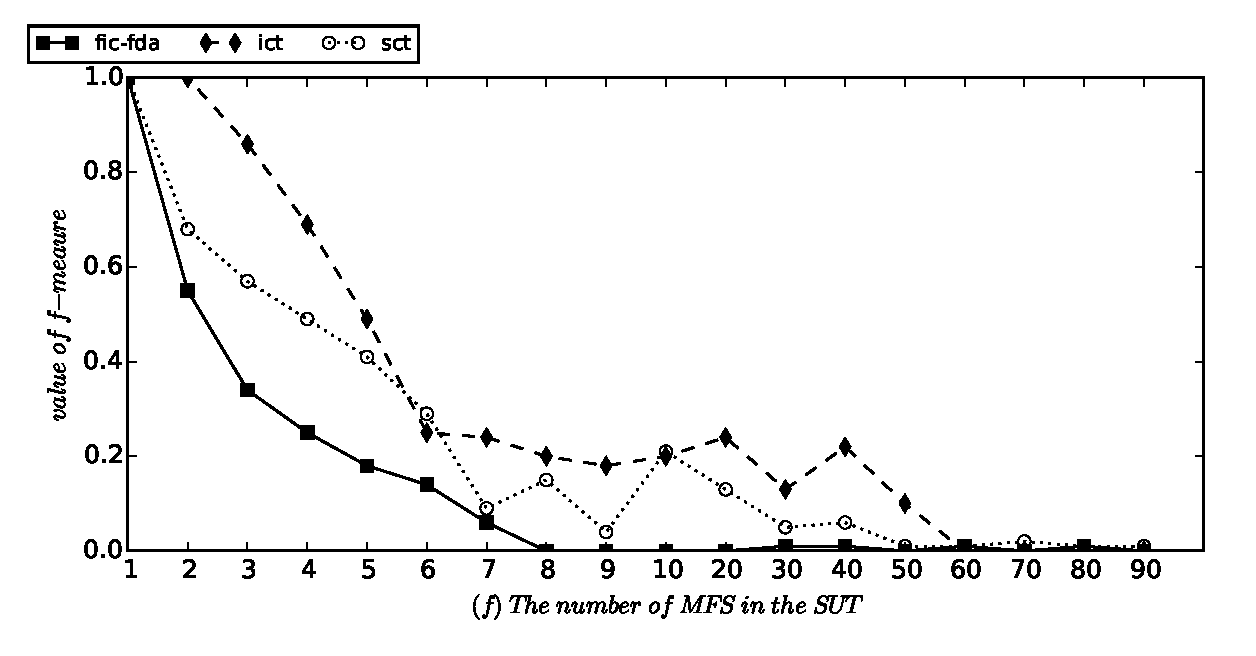
\includegraphics[width=3.5in]{sens_mfs_f_measure.eps}
\caption{F-measure for various number of MFS}
\label{sen_mfs_f_measure_result}
\end{figure}

One observation from Figure \ref{sen_mfs_f_measure_result} is that, with the increasing of the number of MFS, the f-measures of all three approaches decreased rapidly. In fact, when the number of MFS was greater than 60, the f-measures of all three approaches were near 0. This is mainly because if there were too many MFS, it was hard to get a passing test case, and hence, it was challenging to distinguish MFS from those schemas which were not related to the failures.
%This result shows that the number of MFS in SUT do negatively influence the performance of MFS identification.

Another observation is that for most cases, \emph{ict} performed the best, then followed \emph{sct}, and the last was \emph{fda-cit}. It is clear that \emph{ict} can work well under the condition of multiple MFS when compared with the other two approaches.

%Above all, the result shows that the number of MFS in SUT do negatively influence the performance of MFS identification.


\begin{figure}[htbp]
 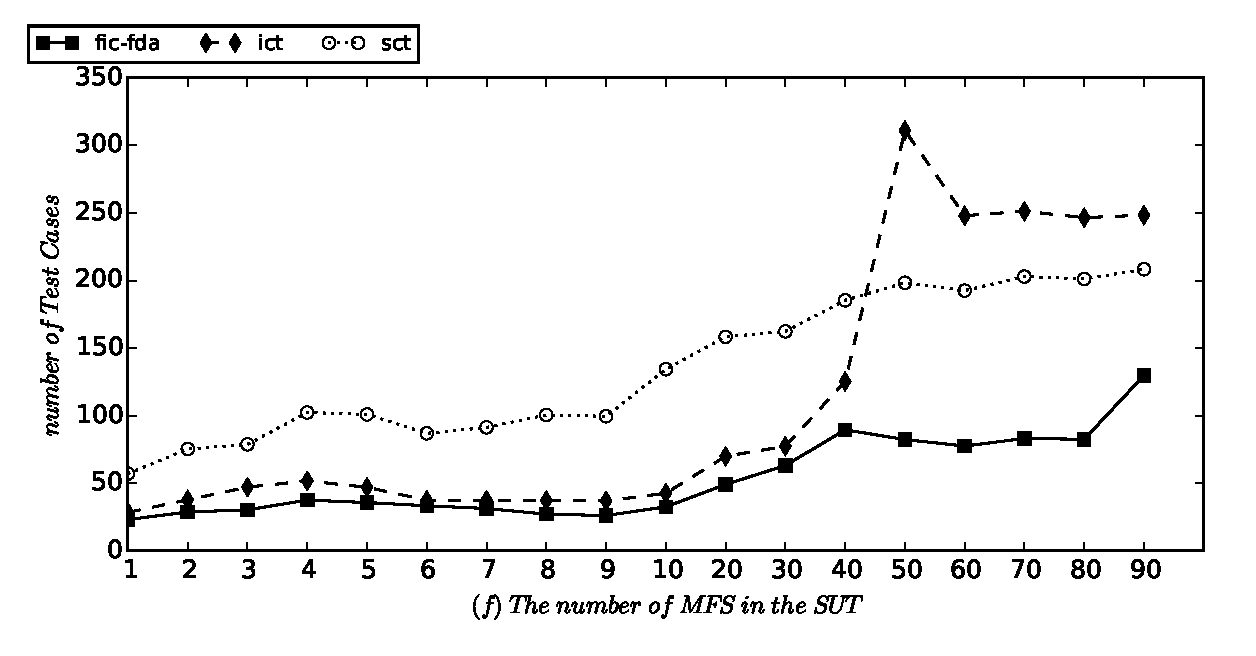
\includegraphics[width=3.5in]{sens_mfs_tests.eps}
\caption{Test Cases for various number of MFS}
\label{sen_mfs_tests_result}
\end{figure}


With regard to the cost, one observation is that with the increasing of the number of MFS, all three approaches needed more test cases to identify the MFS. The reason is also obvious -- a high number of MFS can trigger more failing test cases, and in this situation, approaches needed more additional test cases for MFS identification. For \emph{fda-cit}, even though it did not need additional test cases for MFS identification, a high number of MFS would lead to slower convergence. This is because it is harder to fulfill the \emph{tested-t-way} coverage if there are too many failing test cases, and the slower convergence will surely result in generating more test cases.


%%%%%%-----
Another observation about the cost is that \emph{ict} generated the smallest size of test cases when compared to the other two approaches. In fact, when the number of MFS was greater than 20, the cost of \emph{sct} and \emph{fda-cit} increased rapidly (reached to about 500 test cases), which far exceeded that of \emph{ict}.


{\color{red}
Now lets see see

\begin{figure}[htbp]
 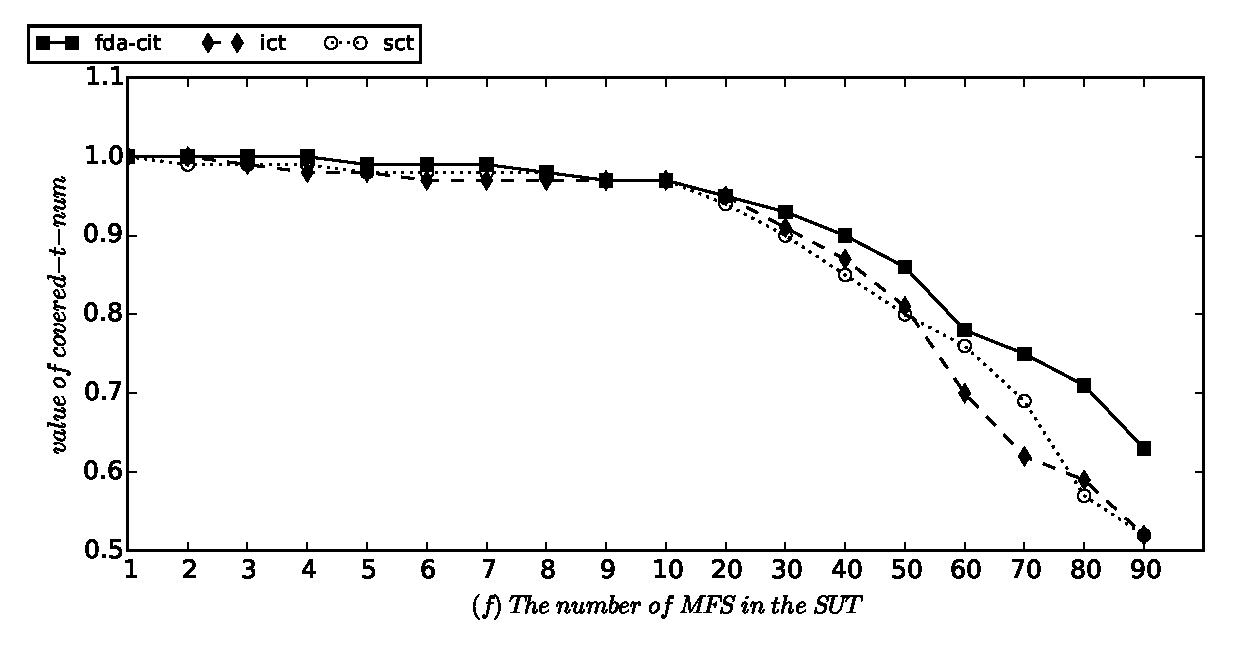
\includegraphics[width=3.5in]{num_mfs_t_tuple.eps}
\caption{number of tested-t-tuples}
\label{sen_mfs_t_tuple_result}
\end{figure}
}



Considering that approaches \emph{ict} and \emph{sct} need to identify the MFS in each of the failing test cases which may contain single MFS or multiple MFS, it is very interesting to observe the performance for these two approaches on the test cases that containing multiple MFS only. Hence, we filtered the results obtained from those failing test cases that only contain single MFS, and focused on those test cases that contain multiple MFS. The MFS identification results (multiple MFS) are listed in Figure \ref{sen_mfs_multi_tests_result}. Additionally, we attached the decrease of f-measure of these two approaches when compared with the results on the test cases that are  not distinguished by containing single MFS and multiple MFS in Figure \ref{decrease_sen_mfs_multi_tests_result}. Note that there is no data at 1 on the x-axis because there is no test case containing multiple MFS in this condition (the SUT only contains one MFS).

\begin{figure}[htbp]
 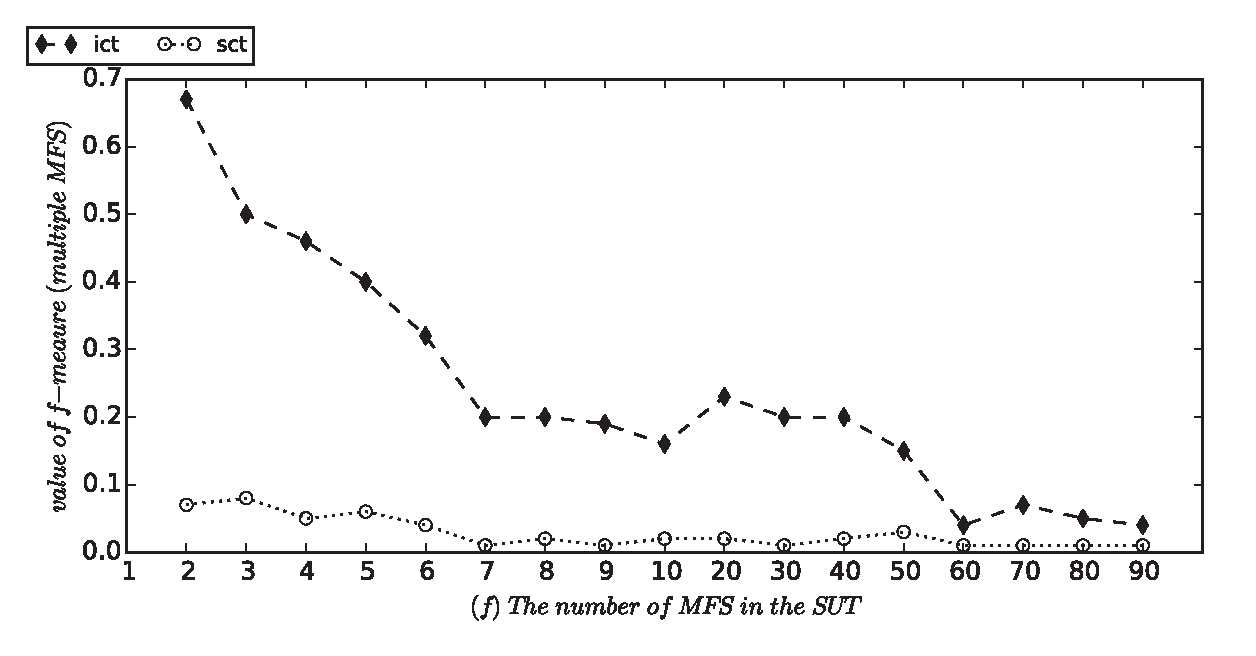
\includegraphics[width=3.5in]{fmeasuremulti.eps}
\caption{F-measure (multiple MFS in one test case) for various number of MFS}
\label{sen_mfs_multi_tests_result}
\end{figure}

\begin{figure}[htbp]
 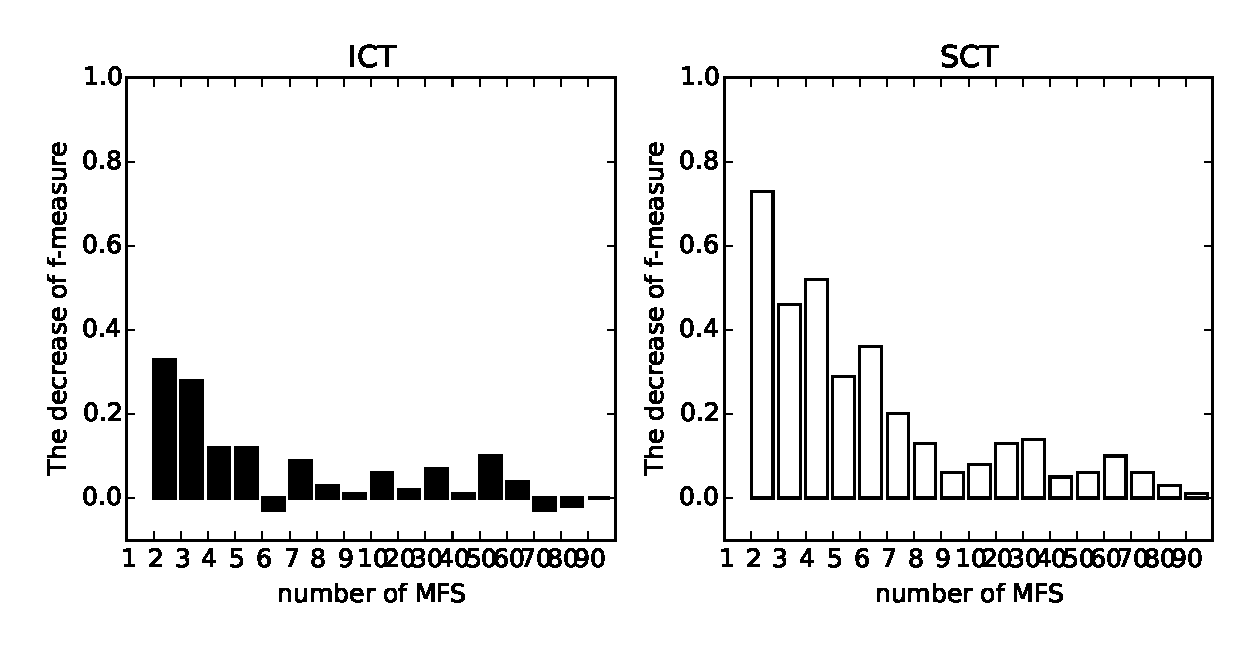
\includegraphics[width=3.5in]{decreasingoffmeasure.eps}
\caption{The decrease of F-measure (multiple MFS in one test case) for various number of MFS}
\label{decrease_sen_mfs_multi_tests_result}
\end{figure}

We can first observe that approach \emph{ict} outperformed \emph{sct} on MFS identification on test cases that containing multiple MFS. In fact, for all the cases listed in Figure \ref{sen_mfs_multi_tests_result}, \emph{ict} obtained higher scores of f-measure than \emph{sct} (note that for all the cases, the f-measure of \emph{sct} is under 0.1). The gaps between them are ranged from 0.05 to 0.69, which is not trivial. Second, the condition that multiple MFS appear in one test case has large negative effects on \emph{sct}, while only has a relatively slight influence on \emph{ict}. Specifically, the decrease of f-measure of \emph{sct} (when compared with the f-measure obtained by \emph{sct} on test cases that are not distinguished by single MFS and multiple MFS) is ranged from 0.01 to 0.73, while the decrease of f-measure of \emph{ict} is no more than 0.32. In fact, there are three cases (x-axis of 6, 80, and 90) on which \emph{ict} even performed better than before.


% which is much smaller cost than that of \emph{sct}. This result is consistent with what we had already obtained in Section \ref{sec:emprical:CompareFDA}.

%always needs the least number of test cases. This is because \emph{fda-cit} does not needs
%The reason of this decline is that when MFS increases, almost all the test cases fail, and hence, the advantage that \emph{ict} triggers fewer failing test cases will disappear. On the other hand, the more the failing test cases are generated, the harder \emph{ict} can reach the coverage (because failing test cases do not contribute to the overall coverage). Hence, \emph{ict} has to generate much more test cases than \emph{sct} when the number of MFS reaches a vey large fraction.

Above all, with the increasing of the number of MFS in the SUT, the performance of all three approaches decreased, but \emph{ict} still performed better than the other two approaches.

%A endition condition

\subsubsection{Number of options}
The results for the sensitivity of the number of options are shown in Fig. \ref{sen_opts_f_measure_result}, Fig. \ref{sen_opts_tests_result} and Fig. \ref{sen_option_t_tuple_result}, which depicts the quality of MFS identification, the number of generated test cases, and the results of masking effects, respectively.
%Note that we do not show the MFS identification result because all three approaches obtain 1.0 of f-measures for all the cases. It shows that the number of  options in the SUT does not influence the quality of MFS identification.
%%%%%%%%%%%%%----%%%%%%%%%%%%%%%%%%%%%%%%%%%%%%%%%%%%%%%%%%%%%%%%%%%%%%%%%%%%

\begin{figure}[htbp]
 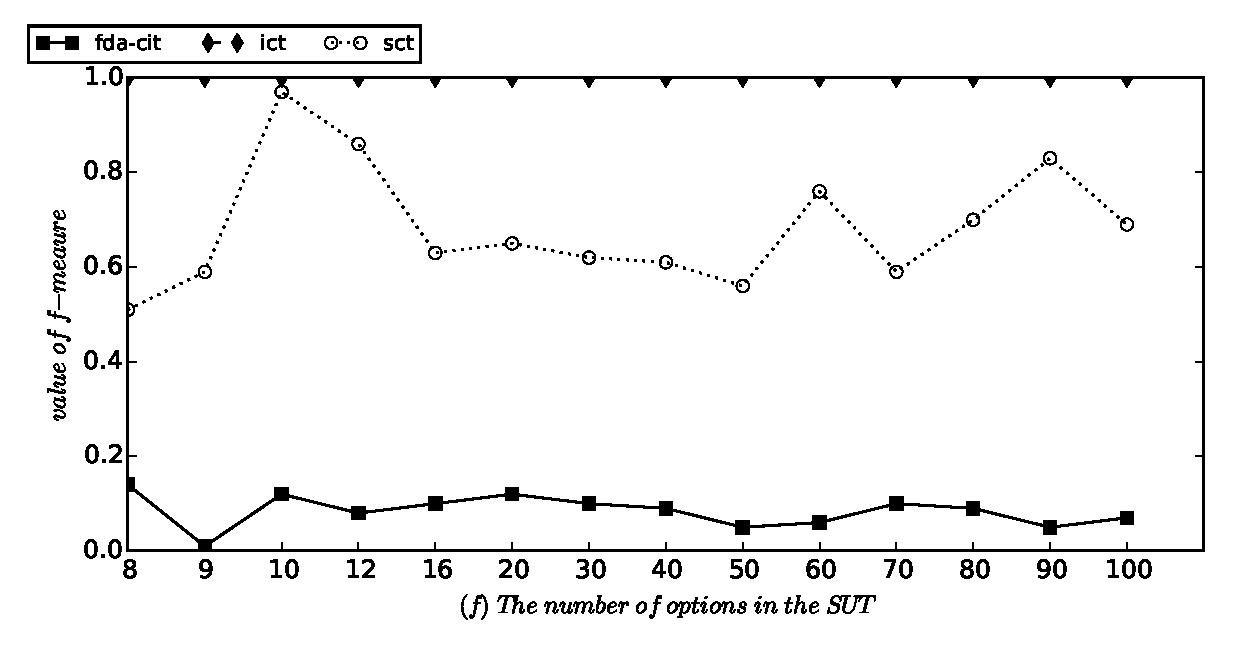
\includegraphics[width=3.5in]{sens_options_f_measure.eps}
\caption{F-measure for various number of options}
\label{sen_opts_f_measure_result}
\end{figure}


\begin{figure}[htbp]
 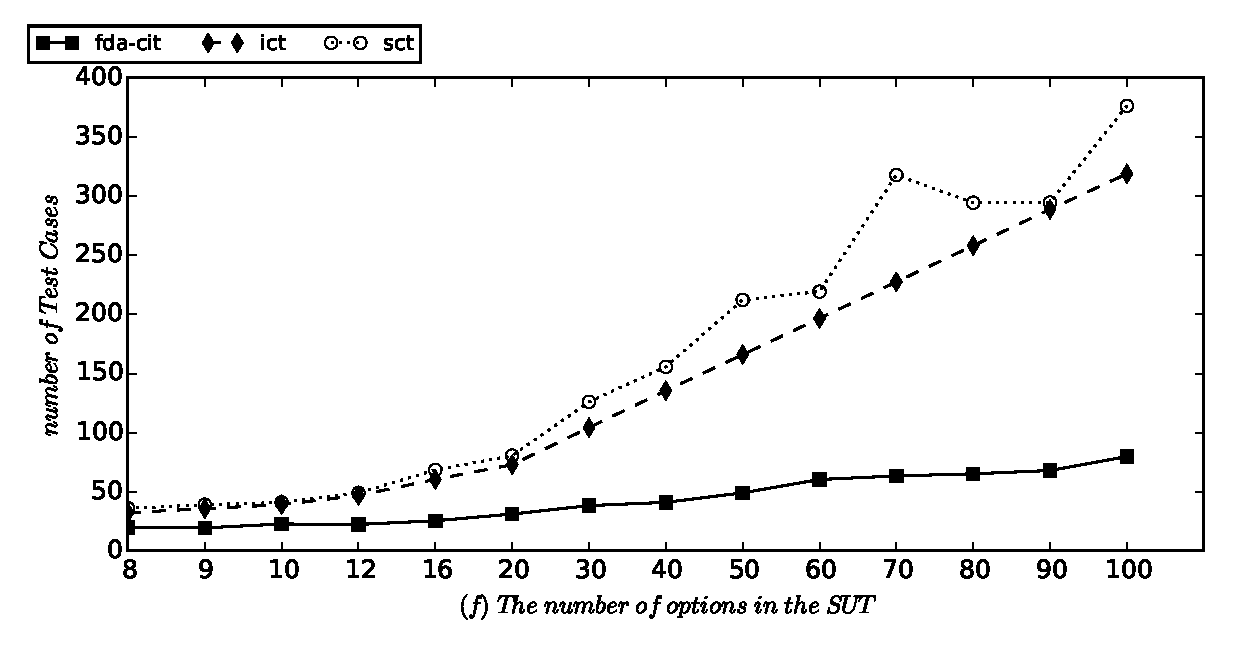
\includegraphics[width=3.5in]{sens_options_tests.eps}
\caption{Test Cases for various number of options}
\label{sen_opts_tests_result}
\end{figure}

\begin{figure}[htbp]
 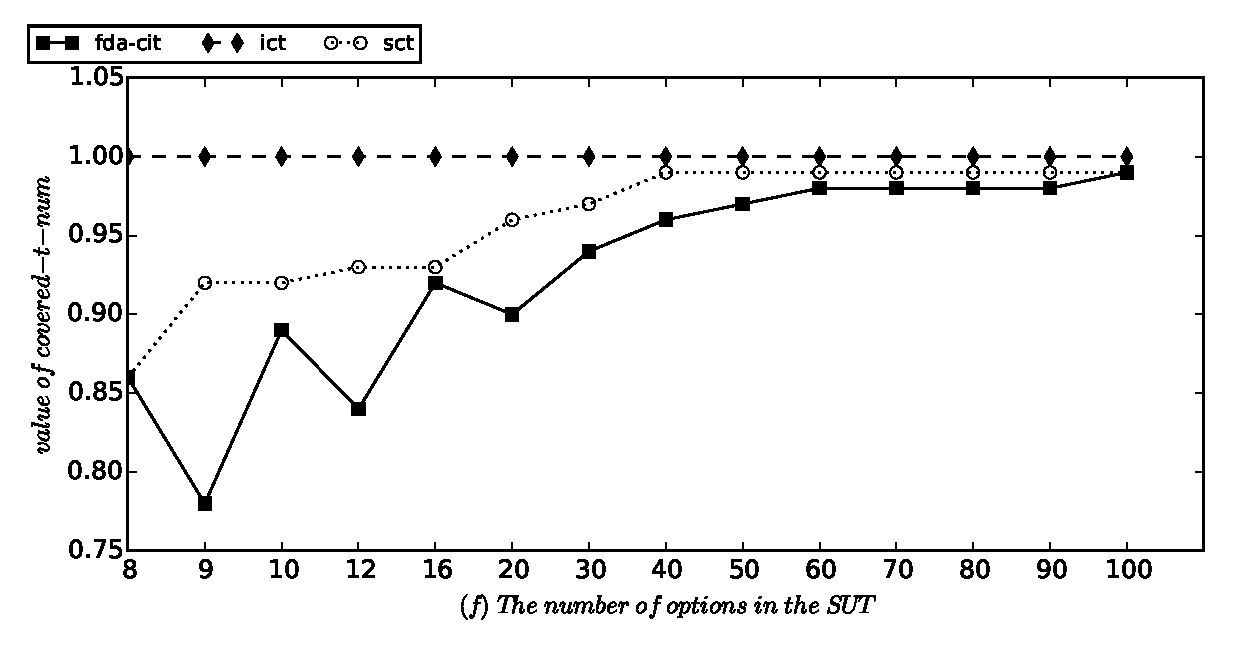
\includegraphics[width=3.5in]{num_option_t_tuple.eps}
\caption{number of tested-t-tuples}
\label{sen_option_t_tuple_result}
\end{figure}

With regard to the quality of MFS identification, it is clear that \emph{ict} performed the best, then followed \emph{sct}, and the last was \emph{fda-cit}. In fact, for all the subjects, \emph{ict} scored 1.0 of f-measure, which indicates that \emph{ict} accurately identified all the MFS. On the other hand, \emph{sct} scored around 0.5 to 0.9, and \emph{fda-cit} only scored around 0.1.  This result is consistent to the previous study, indicating that \emph{ict} can accurately identify the MFS, even though when the number of options is large.

Another observation about the MFS identification is that there was no clear correlation between the MFS quality and the number of options. In fact, there were no clear regularities for the curves representing the f-measures of \emph{sct} and \emph{fda-cit} with the increasing of the number of options. It shows that the number of options in the SUT did not have influence on the quality of MFS identification.

With regard to the number of test cases, there was a clear trend that \emph{fda-cit} performed the best, of which the number of needed test cases grew slowly. This is mainly because it did not generate additional test cases for MFS identification. The second best was \emph{ict}, as the number of test cases increased linearly with the number of options in the SUT. This is due to the mechanism of the MFS identification approach applied in the \emph{ict} framework, i.e., we must always generate the same number of test cases as the number of options in the SUT to identify the MFS. The complexity can be further reduced (O(log N)\cite{zhang2011characterizing,li2012improved,niu2013identifying}). The last one was \emph{sct}, of which the number of test cases was always larger than that of \emph{ict}.


{\color{red}
Now lets see see


}



Therefore, the number of options in the SUT did not have influence on the quality of MFS identification; and although generating more test cases than \emph{fda-cit}, \emph{ict} was still a better choice when considering the precision and recall of MFS identification.

In summary, the answer to Q6 is:
\textbf{Large number of MFS has a negative impact on the quality of the MFS identification of all the three approaches, while the number of options does not. Additionally, \emph{ict} performs best among the three approaches for various number of MFS and options.}

\subsection{The ability of handling assumptions}\label{sec:emprical:Assumption}
The last study is designed to evaluate the performances of the three approaches when the two assumptions proposed on Section \ref{sec:back:iden}, i.e., deterministic failures and the existence of safe values,  do not hold.
%a very common case in practice which is highly relevant to the suggested framework is that of a test space that contains many MFS of a low degree.

\subsubsection{Study setup}
The same as the previous study, in order to make the characteristics of the SUT under control, we decided to use synthetic subjects instead of real programs in this case study. Particularly, synthetic subjects can be injected with various types of faults, e.g., the non-deterministic failures with various probabilities that can be triggered during testing, such that it helps us to evaluate the performance of these approaches for various extent to which these two assumptions do not hold. As a result, we can obtain a more general conclusion instead of those results based on some specific programs.

Specifically, for the first assumption, we decided to inject the MFS that is non-deterministic (the test case which contains it may fail or may not after execution). Then we considered the following possible probabilities that the non-deterministic MFS may be triggered (The probability that the test case which contains it fails after execution): 0.01, 0.05, 0.1, 0.15, 0.2, 0.3, 0.4, 0.5, 0.6, 0.7, 0.80, 0.9, and 0.98, respectively. We repeated the experiment 30 times for each probability to avoid the random affects. For each run of the experiment, we applied all the three approaches on the subject and recorded their results (MFS identification quality and cost).

The second study is to evaluate the performance of approaches when the safe value assumption does not hold. In fact, in our previous studies, the safe value assumption was also not always hold. For example, in the first study, we did not give any safe value to our approach \emph{ict}. Instead, we just generated additional test cases containing the schemas under test. As a result, we did not always reach the 100\% f-measure of MFS identification. For this study, we decided to evaluate these approaches on the condition that there is none safe value, i.e., every parameter value is contained in at least one MFS. We used synthetic subjects with  the input model, and the information of MFS are listed in Table \ref{inputs_non_safe}. The same as Table \ref{inputs}, input model is presented in the abbreviated form $\#values^{\#number\ of\ parameters} \times ...$, and  Column ``MFS" shows the degrees of each MFS and the number of MFS (in the parentheses) with that corresponding degree. Then we applied the three approaches on each subject and compared their performance under the condition that there is non-safe value in each subject.

\begin{table}[ht]
\caption{Inputs model for experiments of non-safe value}
\label{inputs_non_safe}
\centering
\begin{tabular}{l|l|l}
\hline
Subjects & Inputs & MFS \\
\hline
Syn1   &  $4^{8}$       & 2(6)\ 6(4)  \\
Syn2   &   $4^{10} $      &  2(10)\ 6(4) \\
Syn3     &   $4^{12} $      &    2(6)\ 3(4)\ 7(4)  \\
Syn4    & $4^{16}$        &  2(2)\ 3(4)\ 5(4)\ 8(4)   \\
Syn5     &  $4^{20}  $ &2(10)\ 7(4)\ 9(4) \\
Syn6   &  $4^{25}$       & 2(10)\ 9(4)\ 12(4)  \\
Syn7   &   $4^{30}$      &  2(6)\ 3(4)\ 10(4)\ 15(4) \\
Syn8     &   $4^{35} $      & 2(6)\ 6(4)\ 10(4)\ 17(4)  \\
Syn9    & $4^{40} $        &   2(6)\ 8(4)\ 13(4)\ 17(4)   \\
Syn10     &  $4^{50} $ &2(6)\ 13(4)\ 15(4)\ 20(4) \\ \hline
\end{tabular}

\end{table}
%Details of each subject can be seen
%%%%%%%%%%%%%----%%%%%%%%%%%%%%%%%%%%%%%%%%%%%%%%%%%%%%%%%%%%%%%%%%%%%%%%%%%%

\subsubsection{Non-deterministic failures}
The results of evaluating the approaches on non-deterministic failures are shown in Fig. \ref{sen_und_f_measure_result}, Fig. \ref{sen_opts_tests_result}, and Fig. \ref{sen_pro_t_tuple_result}, of which the first figure depicts the quality of MFS identification with various probabilities that the non-deterministic failures are triggered, the second figure shows the number of test cases, and the last one shows the results of the masking effects.

\begin{figure}[htbp]
 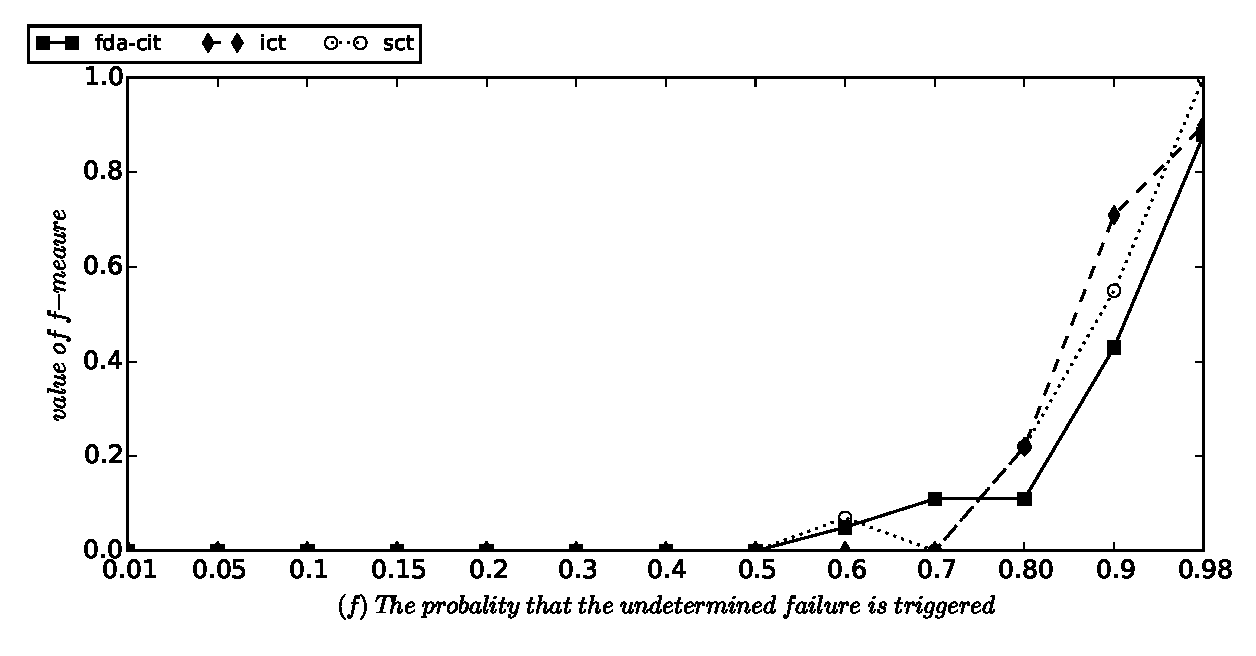
\includegraphics[width=3.5in]{sen_und_f_measure.eps}
\caption{F-measure for various probability of un-determining failure}
\label{sen_und_f_measure_result}
\end{figure}


\begin{figure}[htbp]
 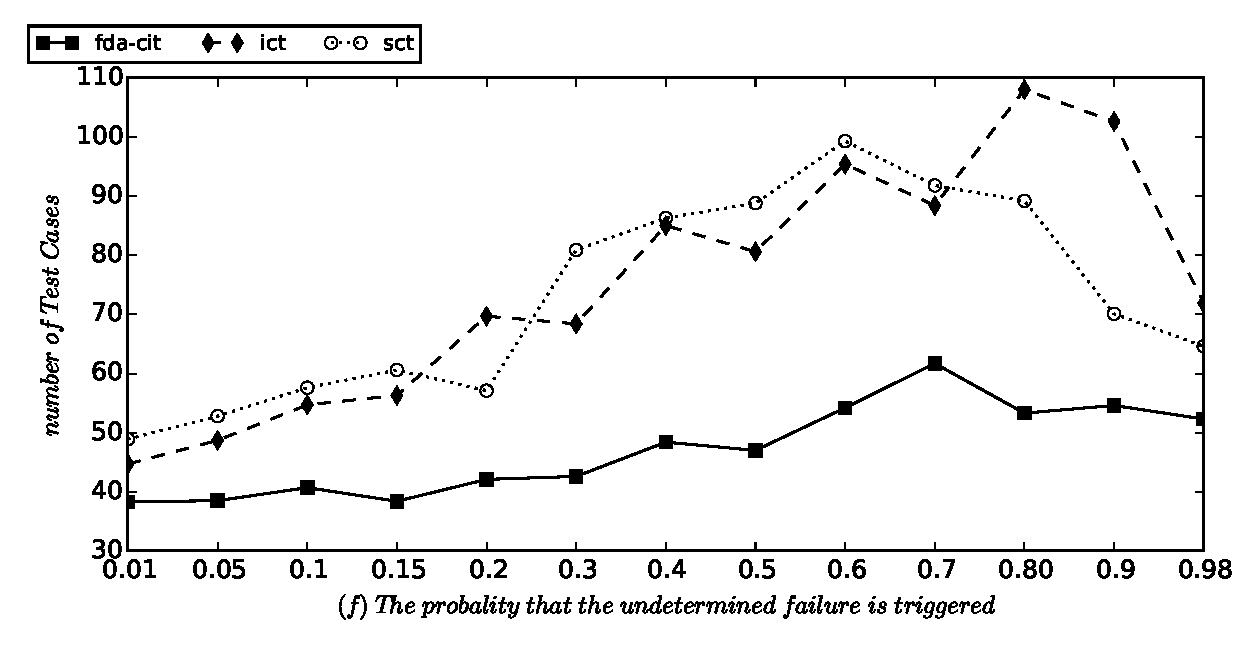
\includegraphics[width=3.5in]{sen_und_tests.eps}
\caption{Test Cases for various probability of un-determining failure}
\label{sen_und_tests_result}
\end{figure}

\begin{figure}[htbp]
 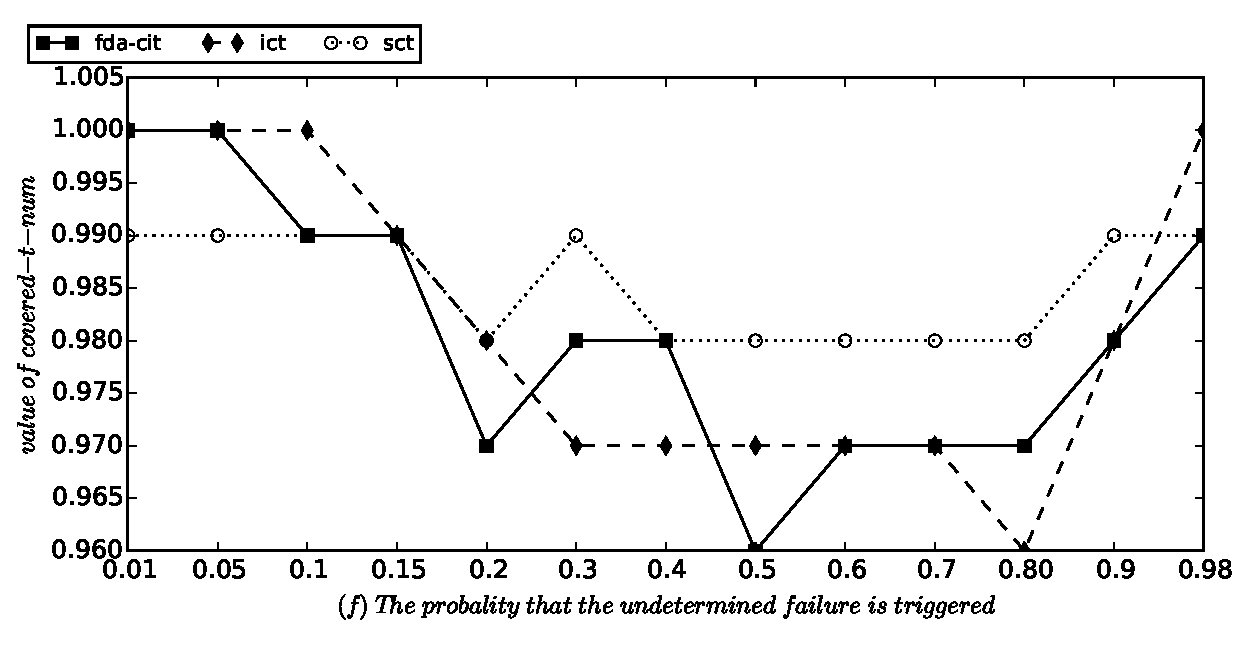
\includegraphics[width=3.5in]{sen_pro_t_tuple.eps}
\caption{number of tested-t-tuples}
\label{sen_pro_t_tuple_result}
\end{figure}

With regard to MFS identification, there are two observations. First, if the probability was below 0.5, all the three approaches did  not identify any MFS at all (with f-measure of 0). We believe there are two possible reasons for the low f-measure of all the three approaches. The first one is that if the probability of triggering MFS was too small (below 0.2), approaches could hardly detect the failure, and hence could not identify the MFS. Another one is that if the probability of triggering MFS is around 0.5, then the failure may appear at one testing, but disappear at the next time. These two statues exchanged frequently and resulted in a negative influence on the MFS identification.
%As a result, the MFS was similar to a non-failure inducing schema, and hence it had little influence on the MFS identification. On the other hand, if the probability was too high, which indicated that approaches could easily detect it. Under this condition, the failure was similar to a deterministic failure, which also had little influence on the MFS identification. The worst condition was in between (the probability was around 0.3 to 0.8). Under such condition, the failure may appear at one testing, but disappear at the next time. These two statues exchanged frequently, and resulted in a negative influence on the MFS identification.


The second observation is that when the probability of triggering MFS was larger than 0.5, the f-measure of all the three approaches increased. In fact, when the probability of triggering MFS was larger than 0.9,  the f-measure of all the three approaches was more than 0.4. We believe if the probability was relatively high, then all the three approaches could easily detect it. Under this condition, the failure was similar to a deterministic failure, which also had little influence on the MFS identification.
%{\color{blue}This result indicates that \emph{ict} can handle the non-deterministic failures properly.}

%Note that the low f-measures of \emph{fda-cit} do not indicate that \emph{fda-cit} cannot deal with non-deterministic failures, instead, it is caused of the proosed meachm to handle the non-determineistic, for example, . There is only one reason, that is the MFS identniciton CTA is not suitable for fault localziotn in combaintoeiatl testing.

With regard to the test cases, our conclusion is similar to the previous study, that is, \emph{fda-cit} needed the smallest amount of test cases, then followed the \emph{ict} and \emph{sct}.

{\color{red}let me see see}

Since the non-deterministic failures have negative effects on MFS identification, it is desirable to alleviate the effects. In this paper, we consider the redundancy of test case execution, i.e., we repeatedly run one test case to check whether it fails or not instead of just one time. We conducted an additional experiment to evaluate the performance of this strategy. Specifically, all the experimental set-ups are as the same as the previous experiment on non-deterministic failures, except that we set the redundancy of test execution to be 5 (run 5 times for each test case).

Figure \ref{sen_und_f_measure_result_reduncy} shows the results. From this figure, we can easily learn that for all these three approaches, there was a significant improvement in the quality of MFS identification. In fact, all these three approaches start to identify at least one MFS among 30 times even the probability of triggering MFS was as low as 0.2. Additionally, when the probability was larger than 0.4, the f-measure of all the three approaches was larger than 0.4. What's more, the f-measure of all the three approaches was close to 1 when  the probability was larger than 0.5.  These results indicated that the redundancy of test case execution is one potential approach to handle the non-deterministic failures problem.
\begin{figure}[htbp]
 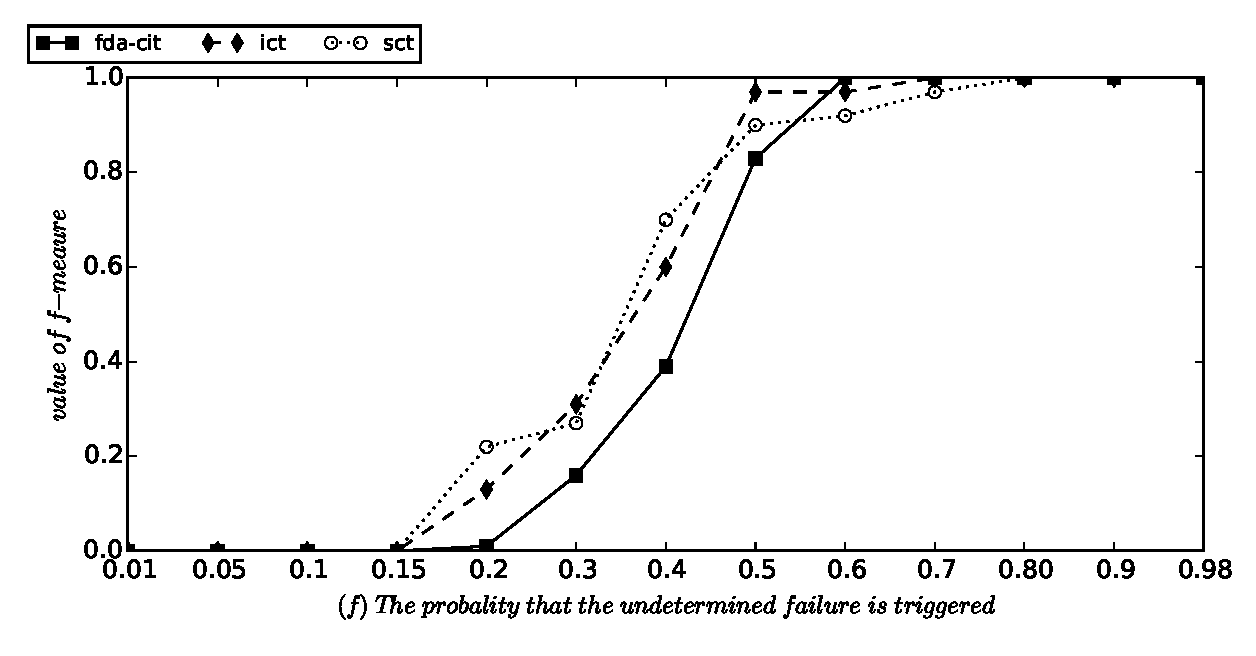
\includegraphics[width=3.5in]{sen_und_redundancy.eps}
\caption{F-measure for various probability of un-determining failure (test execution redundancy of 5)}
\label{sen_und_f_measure_result_reduncy}
\end{figure}


%Above all, we can learn that the non-deterministic failures do affect the MFS quality of the three approaches,  but  {\color{blue}\emph{ict} can handle it well, and perform the best among three approaches.}

%\begin{table*}[ht]
%\caption{Number of test cases contain multiple MFS for \emph{fda-cit}}
%\label{detected_and_fixed_und}
%\centering
%    \begin{tabular}{|l|l|l|l|l|l|l|l|l|l|l|l|l|l|}
%    \hline
%Fixed	&0.0	&185.5	&103.6	&19.8	&30.7	&9.4	&10.6	&4.5	&5.8	&3.7	&4.3	&2.5	&1.9	\\\hline
%Unfixed	&0.0	&0.3	&0.6	&0.7	&1.3	&1.2	&2.0	&1.9	&3.1	&2.7	&3.9	&2.9	&0.5	\\\hline
%    \end{tabular}
%\end{table*}




%%%%%%%%%%%%%----%%%%%%%%%%%%%%%%%%%%%%%%%%%%%%%%%%%%%%%%%%%%%%%%%%%%%%%%%%%%

\subsubsection{Non Safe values}

The results of evaluating the approaches on non-safe values are shown in Fig. \ref{sen_safe_f_measure_result}, Fig. \ref{sen_safe_tests_result}, and Fig. \ref{sen_safe_t_tuple_result}.

\begin{figure}[htbp]
 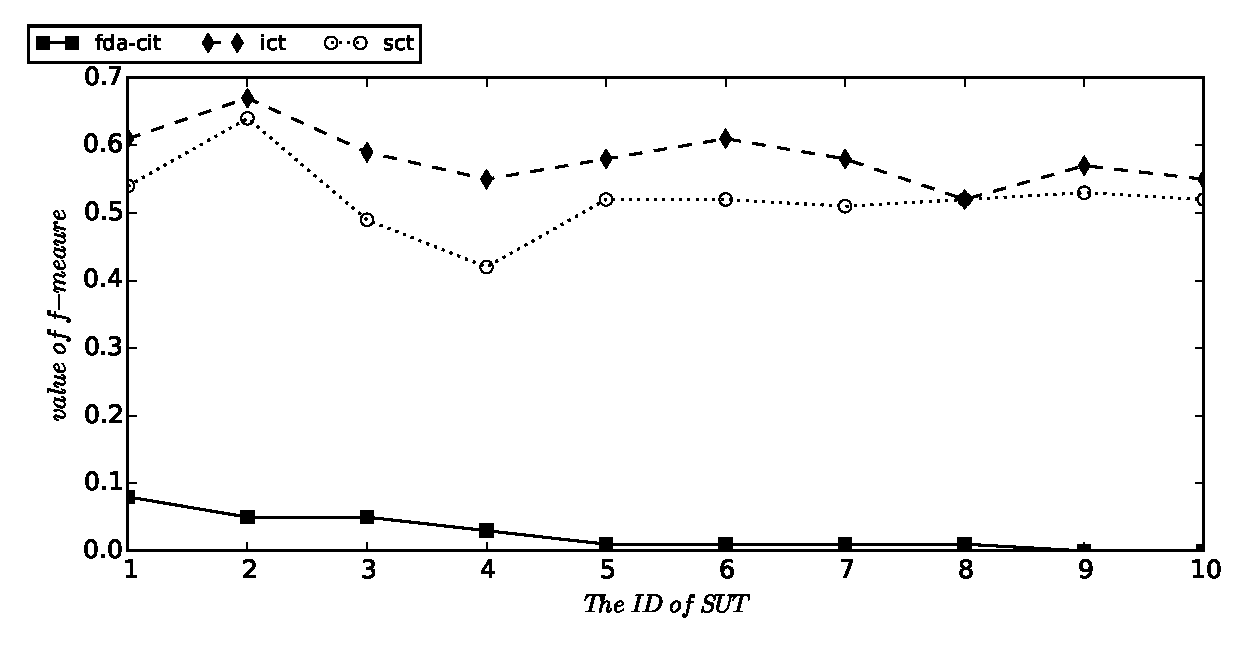
\includegraphics[width=3.5in]{sen_safe_f_measure.eps}
\caption{F-measure for various number of un-safe values}
\label{sen_safe_f_measure_result}
\end{figure}


\begin{figure}[htbp]
 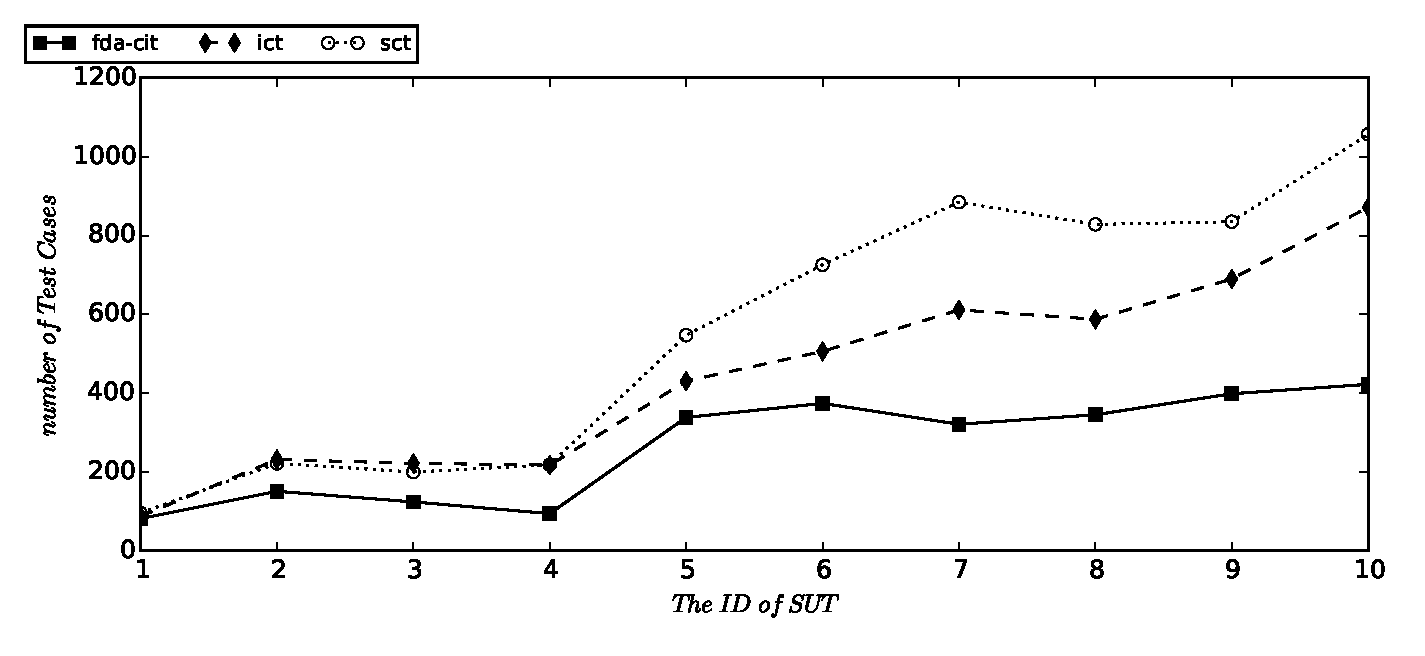
\includegraphics[width=3.5in]{sen_safe_tests.eps}
\caption{Test Cases for various number of un-safe values}
\label{sen_safe_tests_result}
\end{figure}

\begin{figure}[htbp]
 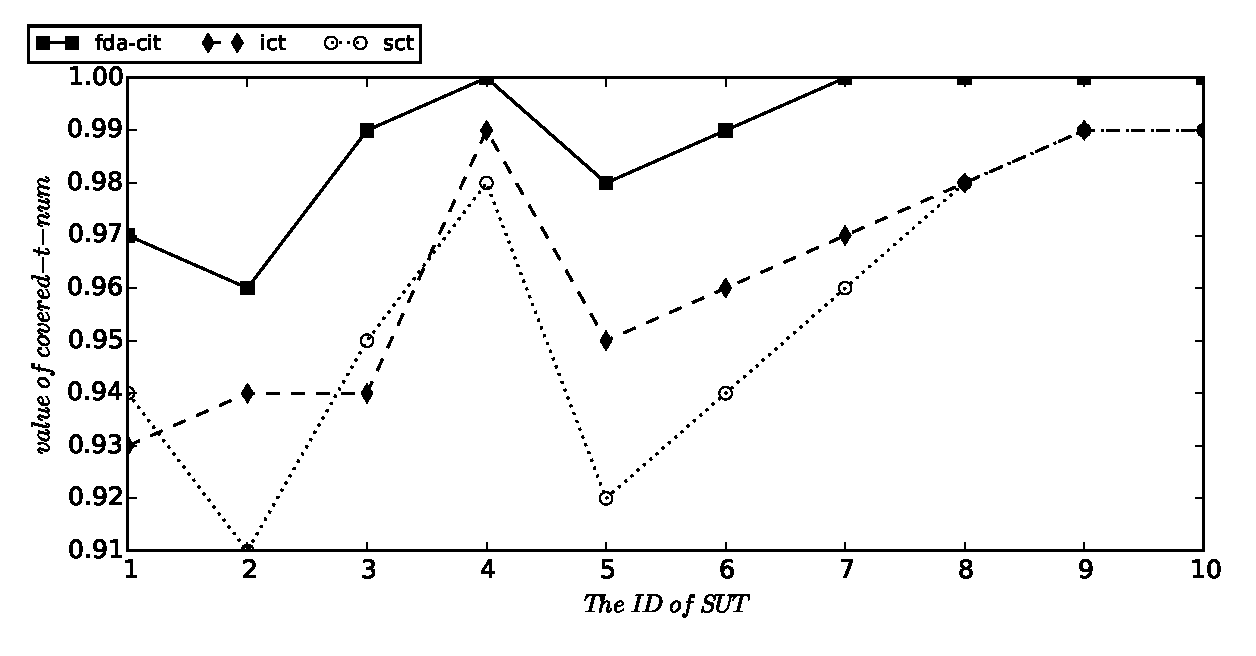
\includegraphics[width=3.5in]{sen_safe_t_tuple.eps}
\caption{number of tested-t-tuples}
\label{sen_safe_t_tuple_result}
\end{figure}

There are several observations about these figures. First, the non-safe values did affect the MFS identification quality of all the approaches. In fact, the f-measures of all the three approaches listed in Fig. \ref{sen_safe_tests_result} were lower than those 0.7. Specifically, \emph{ict}'s f-measure is ranged from 0.52 to 0.67,  \emph{sct}'s ranged from  0.42 to 0.64, and \emph{fda-cit}'s ranged from 0.01 to about 0.08. Based on these data, we can conclude our second observation, that is, \emph{ict} also performed best under the condition that there are no safe values. We believe this is due to our feedback checking process, which significantly improves the quality of MFS identification, and reduces the negative effects caused by non-safe values.
At last, with regard to the number of test cases, \emph{fda-cit} still generated the fewest, but this also led to the low f-measure of MFS identification.

{\color{red}let me see see}
%These results show that the non-safe value have  negative effects on the MFS identification.

Besides these observations, it's also important to figure out how many times that the effects of non-safe values were triggered. More specifically, for the approaches \emph{ict} and \emph{sct} which need to identify the MFS for each of the failing test cases, we need to figure out how many times when these MFS actually caused failures during the MFS identification for one specific failing test case. We listed the results in Figure \ref{sen_safe_NonTrigger} and Figure \ref{sen_safe_NonTriggerAvg}, in which Figure \ref{sen_safe_NonTrigger} recorded the number of total times that the non-safe MFS are triggered for each software subject, while Figure \ref{sen_safe_NonTriggerAvg} recorded average number of times that the non-safe MFS are triggered for each time of MFS identification.

\begin{figure}[htbp]
 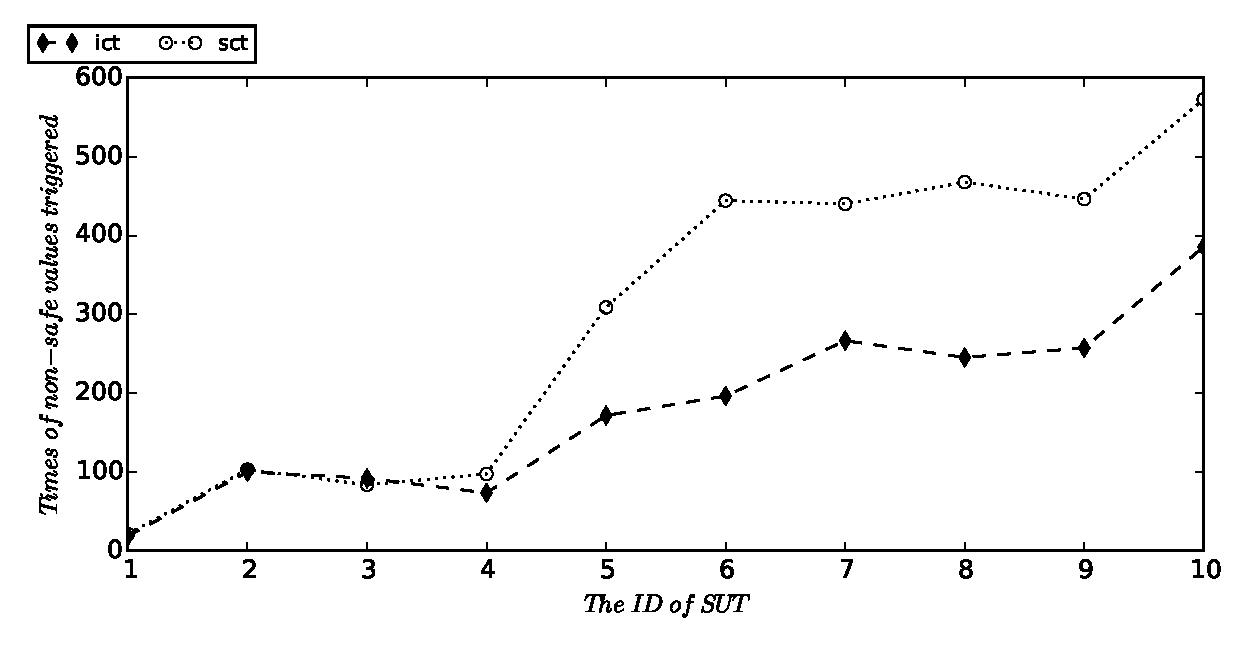
\includegraphics[width=3.5in]{enNonSafe.eps}
\caption{The times of non-safe MFS are triggered in total for each subject}
\label{sen_safe_NonTrigger}
\end{figure}


\begin{figure}[htbp]
 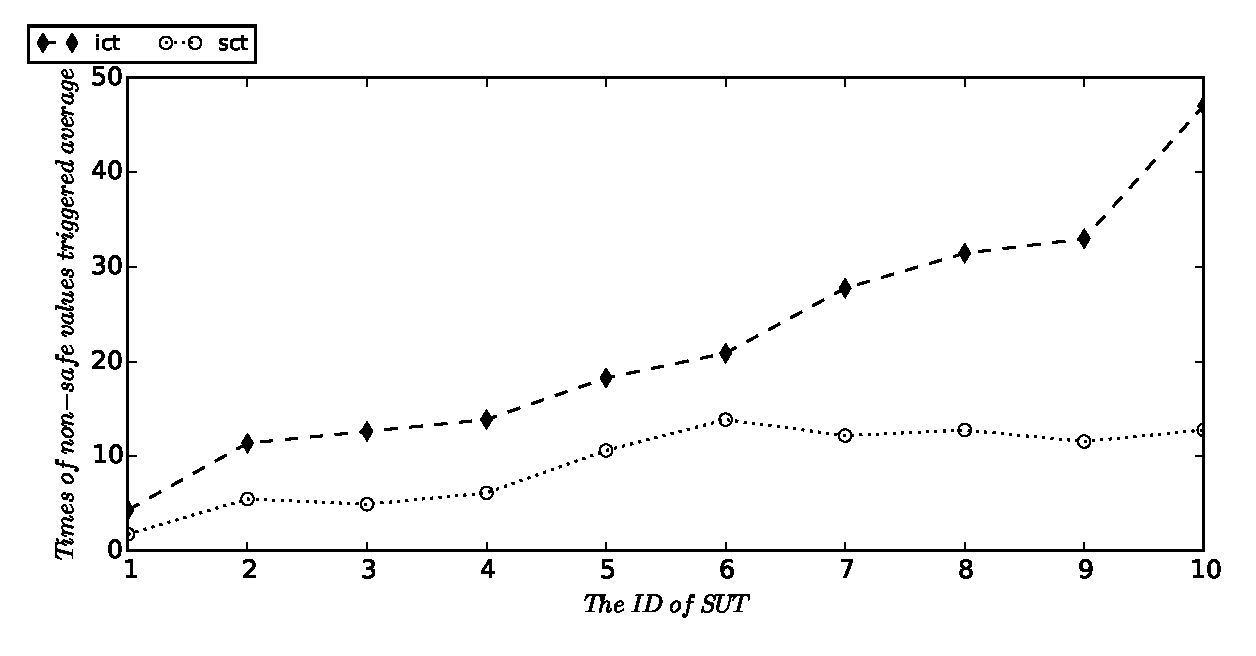
\includegraphics[width=3.5in]{enNonSafeTriggerAvg.eps}
\caption{The times of non-safe MFS are triggered for each time of MFS identification}
\label{sen_safe_NonTriggerAvg}
\end{figure}

Based on these two figures (Figure \ref{sen_safe_NonTrigger} and \ref{sen_safe_NonTriggerAvg}), we can learn that for both of two approaches, the number of times that non-safe MFS was triggered was not trivial. In fact, except for the first subject, the number that non-safe MFS was triggered by these two approaches was both beyond 73.6 times for all the remaining subjects (the maximal non-safe MFS's triggered times of \emph{sct} was up to 572.8, and for \emph{ict}, this number was up to 385.8 ). Additionally, the number that non-safe MFS was triggered for each time that MFS identification was proceeded was still not small. Specifically, for each time of MFS identification, these non-safe MFS were  triggered by about 22 times at average for \emph{ict}, and 7.3 times for \emph{sct}.

%\begin{table*}[ht]
%\caption{Detected and fixed \emph{fda-cit}}
%\label{detected_and_fixed_safe}
%\centering
%    \begin{tabular}{|l|l|l|l|l|l|l|l|l|l|l|l|}
%    \hline
%Fixed	&2.1	&4.9	&3.9	&3.9	&4.0	&4.5	&4.2	&3.9	&3.3	&4.5	&4.9	\\\hline
%Unfixed	&2.4	&3.0	&2.1	&2.1	&2.1	&2.2	&2.0	&2.0	&2.0	&2.2	&2.0	\\\hline
%    \end{tabular}
%\end{table*}

Above all, the answer to the Q7 is:

\textbf{The non-deterministic failures and non-safe values do negatively affect the results of all the three approaches.  Due to the feedback checking process, \emph{ict} can alleviate impacts of the non-safe values. While for non-deterministic failures, one potential solution is the redundancy of test case execution.}



\subsection{Comparison with static error locating arrays}
Considering  that all these approaches evaluated in our previous  experiments are all dynamic approaches (generating test cases), it is interesting to observe how well does the alternative way,  i.e., static error locating arrays, perform on the CT problems.

Error locating array\cite{colbourn2008locating,martinez2009locating} is a well-designed set of test cases that can support not only failure detection but also the identification of the MFS of the failure. It is known that only with a covering array sometimes is not sufficient to identify the MFS, thus additional test cases are needed. Mart{\'\i}nez et al.\cite{martinez2008algorithms} have proved that a $(t + d)$-way covering array can identify all the MFS with the number of them no more than \emph{d}, and degree no more than \emph{t}.
After executing all the test cases in the $(t + d)$-way covering array, the MFS can be obtained by keeping those t-degree or less than t-degree schemas that only appear in the failing test cases.  So with the number \emph{d} and degree \emph{t} known in prior, a $(t + d)$-way covering array is an \emph{Error Locating Array (ELA)}.


To compare our approach with this Error Locating Array is meaningful, as both approaches have the same target. The relationship between our approach with the Error Locating Array can be deemed as the dynamic vs static. In detail, our approach dynamically detects and identifies the MFS in the SUT, i.e., the test cases generated by our approach are changed according to the specific MFS. On the contrary, ELA just generates a static covering array, and it can support MFS identification if the number and degree of these schemas are known in prior.



\subsubsection{Study setup}
In this section, we will  apply ELA to identify the MFS of the 5 subjects in Table \ref{subject}. It is noted that the conclusion that a \emph{(t + d)}-way covering array is an ELA
%In fact, ELA \cite{martinez2009locating,martinez2008algorithms} is a particular covering array. When the maximum degree and number of the MFS are known in prior, say, $t$ and $d$ respectively, then a $(t + d)$-way covering array can support the MFS identification. However, this conclusion
is based on that there must exist \emph{safe} values for each parameter of the SUT. A \emph{safe} value is the parameter value that is not in any part of these MFS. In our experiment, all the five subject programs satisfy this condition. Based on this, we then applied ELA to generate appropriate covering arrays for each subject program and recorded the MFS identified as well as the overall test cases generated. The covering array generation algorithm we adopted in this experiment is also augmenting simulated annealing approach \cite{cohen2003augmenting,cohen2008constructing2}, and similar as previous experiments, this experiment is repeated 30 times.


%Given a configuration space model known to have safe values, a strength t of the interactions to be tested, and an upper bound d on the number of faulty interactions, each of which is assumed to have at most t options, a static (t, d)-way ELA is a traditional (td)-way covering array. If the configuration space model has no safe values, then a static (t, d)-way ELA is a traditional t1-way covering array. Static ELAs, therefore, require that a priori information on the maximum number of faulty interactions is known, otherwise they can suffer from masking effects.



%Additionally, comparisons between the augmented approaches and three traditional ones will be quantified.

\subsubsection{Result and discussion}
First, we list the subject information (the number of MFS $d$ and maximal MFS degree $t$), together with the covering arrays that ELA needs to build, in Table \ref{ela-needs-to-gen}.

\begin{table}[htbp]
\center
\caption{The covering arrays that ELA needs to build for each subject}
\label{ela-needs-to-gen}
\begin{tabular}{|l|l|l|l|l|}
\hline
Subject & t  & d  & t+d & ELA                       \\\hline
Tomcat  & 2  & 3  & 5   & CA(N;5,10,($2^{8} \times 3^{1} \times 4^{1}$))  \\
Hsqldb  & 3  & 3  & 6   & CA(N;6,12,($2^{9} \times 3^{2} \times 4^{1}$))  \\
Gcc     & 3  & 4  & 7   & CA(N;7,10,($2^{9} \times 6^{1}$))      \\
Jflex   & 2  & 1  & 3   & CA(N;3,13,($2^{10} \times 3^{2} \times 4^{1}$)) \\
Tcas    & 12 & 48 & 60  & -      \\ \hline
\end{tabular}
\end{table}
%%%%%%%%%%%%%%%%%%%%%%%%%%%%%%%%%%%%%%%%%%%
From this table, we can learn that for most subjects, ELA needs to build high-way covering arrays. In fact, for tcas, the CA that is needed to be built is 60-way, which is far beyond the number of parameters of TCAS (12) and hence, the corresponding covering array cannot be generated. One exception is Jflex, for which ela needs to build a 3-way covering array. It indicates that the 4-way covering arrays generated for Jflex in the previous experiments are unnecessary. From this point of view, ELA can provide an upper-bound on the strength of the covering arrays that need to be generated for one software subject.


The number of overall test cases, the quality of the identified MFS, and the results of masking effects are listed in Table \ref{cm_ela}. We can firstly observe that this approach needs more test cases than the approaches discussed before. This is as expected becasue this approach needs to generate a higher-way covering array than previous approaches. Apart from the high cost, this approach correctly identified all the real MFS. The accuracy has been proved in \cite{martinez2008algorithms,martinez2009locating}.  Note that this perfect MFS identification result is based on the fact that it knows the number and degree of the MFS at first, which is usually not available in practice.  %On the other hand, other dynamic approaches can get a similar identification result, nbbu
{\color{red} let me see see}


\begin{table*}[htbp]
\center
\caption{Results from Error Locating Array}
\label{cm_ela}
\begin{tabular}{|l|l|l|l|l|l|l|l|}
\hline
Subject & Size   & Precision & Recall & F-measure & Tested-2-way  & Tested-3-way & Tested-4-way \\ \hline
Tomcat  & 210.8  & 1       & 1      & 1      &236.0 (1.0) & 1424.0 (1.0)  & 5450.75 (0.97)    \\
Hsqldb  & 588.8  & 1       & 1      & 1      & 357.0 (1.0) & 2742.0 (1.0) & 14136.0 (1.0)    \\
Gcc      &783.4 & 1       & 1      & 1       & 252.0 (1.0) & 1536.0 (1.0)  &   6048.0 (1.0) \\
Jflex   & 41.8   & 1       & 1      & 1      & 473 (1.0) &4096.75 (0.95)  &  19224.5 (0.72)  \\
Tcas    & - &  -       & -      & -     & -  & - & -   \\ \hline
\end{tabular}
\end{table*}


%We further compare their execution time.
%As both the cost (number of test cases) and the quality of the identified schemas are important in practice, we combine the two metrics (\emph{size} and \emph{f-measure}) by dividing \emph{f-measure} by \emph{size}. The normalized result of this combination metric is shown in Fig.\ref{cm_performance}. In this figure, \emph{ict} and \emph{sct} represent interleaving CT approach and traditional sequential CT approach, respectively. \emph{Ela} indicates the error locating array approach.
%
%\begin{figure}[htbp]
% 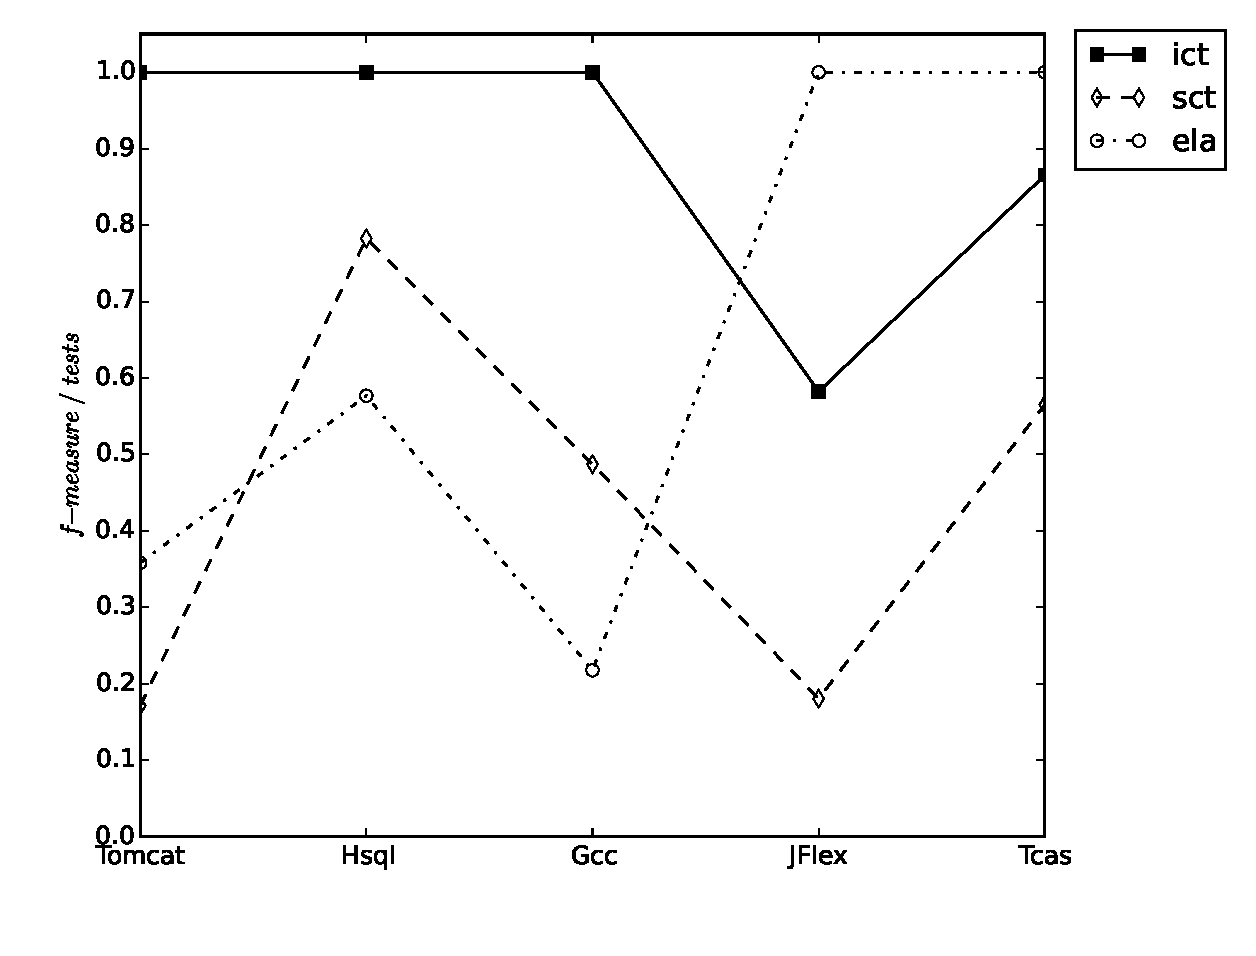
\includegraphics[width=3.4in]{result.eps}
%\caption{Comparison of the combining metric}
%\label{cm_performance}
%\end{figure}

%For \emph{ela}, our approach performs better for three subjects \emph{Tomcat}, \emph{Hsqldb}, and \emph{Gcc}. The reason that our approach does not perform as well as \emph{ela} for subject \emph{JFlex} is that the MFS for that object is a single 2-degree schema (see Table \ref{inputs}), under which ela just needs a 3-way covering array.  For subject \emph{Tcas}, with high-degree MFS as discussed before, our approach is hard to trigger an error with only \emph{2-way}, \emph{3-way}, and \emph{4-way} covering array. As a result, our approach can hardly identify the MFS. Apart from these two special cases, our approach has a significant advantage over the ELA approach.

%One more time, the static way gives us a implication: sometimes we do not need to generate higher-way covering arrays.

In summary, the answer to the Q8 is:

\textbf{ ELA gets the best quality of the MFS identification but needs much more cases than all the other dynamic approaches.  It also needs to know the number and degree of the MFS in prior, which limits its application in practice.}





\subsection{Threats to validity}

There are two threats to validity in our empirical studies. First, our experiments are based on 5 open-source software.  {\color{red} However, these software only represented some specific inputs space and specific degree or location of the MFS. To make the conclusion more general, we need to observe how these approaches performed on other inputs models with different characteristics. For this, we created a batch of synthetic input models.  More specifically, for the synthetic models used in Section \ref{sec:emprical:Sensitivity}, we  consider how approaches performed under a different number of parameters (8 to 100) instead of some specific number of parameters obtained from previous experiments. Additionally, we also consider the different number of MFS (1 to 90) that contained in these synthetic models instead of only 1 or 2. In Section \ref{sec:emprical:Assumption}, these models are created by considering the various probabilities of triggering MFS (1\% to 98\%) instead of 100\% or only some specific probabilities. We also considered the number of times (1 to 47) that unsafe values are introduced each time the MFS identification proceeded in the experiments.}
%More subject programs are desired to make the results more general, such that the conclusion of our experiment can reduce the impact caused by specific input space and specific degree or location of the MFS.

Second, there are many generation algorithms and MFS identification algorithms. In our empirical studies, we just used AETG \cite{cohen1997aetg} as the test case generation strategy and OFOT \cite{nie2011minimal} as the MFS identification strategy. As different generation and identification algorithms may affect the performance of our proposed CT framework, especially on the number of test cases, some studies using different test case generation and MFS identification approaches are desired.
%For test case generation, .     But for OFOT, it can significantly accuracy.


%Third, these empirical studies are all on the deterministic condition, i.e., the output of the software are deterministic if their inputs are given. When the output are affected by random events such that we can not determine the output by only one-time execution of the test case, then both the traditional CT process and our new framework do not work. In such a case, to conduct a test case multiple times or introduce some probability in the framework will be of interest.


\section{related works}\label{sec:related}
Combinatorial testing has been widely applied in practice \cite{kuhn2010practical}, especially on domains like configuration testing \cite{yilmaz2006covering,cohen2006testing,fouche2009incremental} and software inputs testing \cite{cohen1997aetg,borazjany2012combinatorial,garn2014eris}. A recent survey \cite{nie2011survey} comprehensively studied existing works in CT and classified them into eight categories according to the testing procedure. Based on this study, we learn that test case generation and MFS identification are two most important parts in CT studies.

Many works have been proposed for covering array generation, which can be mainly classified into the following four categories \cite{nie2011survey}: 1) greedy methods \cite{cohen1997aetg,lei2008ipog,bryce2005framework,bryce2007density}, which are very fast and effective, but may consume too many test cases.  2) mathematical methods\cite{hartman2005software,kobayashi2002design,williams2000determination,williams2002formulation}, which can also be extremely fast and can produce optimal test sets in some special cases, but they impose many restrictions. 3) Heuristic search techniques \cite{bryce2007one,cohen2003augmenting,cohen2003constructing,ghazi2003pair,shiba2004using,wu2015discrete} , which can generate very small size of test cases, but may cost much computation time and 4) random methods \cite{schroeder2004comparing,nie2015combinatorial}, which are extremely fast, but generate more test cases than greedy approaches.

The MFS identification problem also attracts many interests in CT. These approaches for identifying MFS can be partitioned into two categories \cite{colbourn2008locating} according to how the additional test cases are generated: \emph{adaptive}--additional test cases are chosen based on the outcomes of the executed tests \cite{shi2005software,nie2011minimal,ghandehari2012identifying,niu2013identifying,zhang2011characterizing,shakya2012isolating,wang2010adaptive,li2012improved}or \emph{nonadaptive}--additional test cases are chosen independently and can be executed in parallel \cite{yilmaz2006covering,colbourn2008locating,martinez2008algorithms,martinez2009locating,zhang2012faulty}.
%###################qu2008configuration, ghandehari2013applying,

%took a survey on the studies about different aspects of combinatorial testing, and based on which, we can learn that many works in CT focus on separately aspects, i.e. either focus on generation, or on evaluation or on fault localization, or on building models .

Although CT has been proven to be effective at detecting and identifying the interaction failures in SUT, however, to directly apply them in practice can be inefficient and sometimes even does not work at all. Some problems, e.g., constraints of parameters values in SUT \cite{cohen2007exploiting,cohen2008constructing}, masking effects of multiple failures\cite{dumlu2011feedback,yilmaz2013reducing}, dynamic requirement for the strength of covering array \cite{fouche2009incremental}, will cause difficulty to the CT process. To overcome these problems, some works try to make CT more adaptive and flexible.

%Tere are several drawbacks for traditional CT studies. First, not practical, not. To overcome this, several works are proposed to extend CT to make them better application.
%To avoid this,
%the methodology, notions and in CT.
%On this filed, most works separately discussed , such as.

JieLi \cite{li2012improved} augmented the MFS identifying algorithm by selecting one previous passing test case for comparison, such that it can reduce some extra test cases when compared to another efficient MFS identifying algorithm \cite{zhang2011characterizing}.

S.Fouch{\'e}  et al., \cite{fouche2009incremental} introduced the notion of incremental covering array. Different from traditional covering array, it does not need a fixed strength to guide the generation; instead, it can dynamically generate high-way covering array based on existing low-way covering array, which can support a flexible tradeoff between the covering array strength and testing resources. Cohen \cite{cohen2007exploiting,cohen2008constructing} studied the impacts of constraints on CT, and proposed an SAT-based approach that can handle those constraints.  Bryce and Colbourn \cite{bryce2006prioritized} proposed an one-test-case-one-time greedy technique to not only generate test cases to cover all the $t$-degree interactions, but also prioritize them according to their importance.  E. Dumlu et al., \cite{dumlu2011feedback} developed a feedback driven
combinatorial testing approach that can assist traditional approaches in avoiding the masking effects between multiple failures. Yilmaz \cite{yilmaz2013reducing} extended that work by refining the MFS diagnosing method. Specifically, this feedback driven approach firstly generates a $t$-way covering array, and after executing them, the MFS will be identified by utilizing a classification tree method. It then forbids these MFS and generates additional test cases to cover the interactions that are masked by the MFS. This process continues until all the interactions are covered. Additionally, Nie \cite{nie2013adaptive} constructed an adaptive combinatorial testing framework, which can dynamically adjust the inputs model, strength $t$ of the covering array, and the generation strategy during CT process.

Our work differs from the above studies mainly in that we proposed a highly interactive framework for test case generation and MFS identification. Specifically, we do not generate a complete $t$-way covering array at first; instead, when a failure is triggered by a test case, we immediately terminate test case generation and turn to MFS identification. After the MFS is identified, the coverage will be updated and the test case generation process continues.

Besides the works on fault localization in combinatorial testing, some code-based fault localization studies also show some similarities with our work. Existing code-based fault localization can be mainly classified into two categories \cite{robetaler2012isolating}:  First, \emph{statistical}
approaches \cite{jones2002visualization,liblit2003bug,liu2005sober}.  These approaches utilize the coverage of statements or other program entities in the execution traces of failed and passed tests to compute suspiciousness of each statement or other program entities. Then they will rank these program entities according to their likelihood of containing the defect, i.e., the computed suspiciousness scores. These approaches are effective, but may need sufficient test cases execution results. Second, \emph{experimental} approaches\cite{zeller2002simplifying,zeller1999yesterday,misherghi2006hdd}. By altering some inputs, code, or some other entities, these approaches can generate additional test cases. By comparing these test cases, as well as the testing outcomes, the failure-inducing parts of the test cases will be isolated. In fact, two MFS identification approaches are directly inspired by the delta debugging ideas \cite{zhang2011characterizing,li2012improved}. Additionally, a study \cite{ghandehari2013fault} initially combines the MFS identification approach with code-based localization techniques to obtain a better fault isolation result.

From these works, the idea in BugEx \cite{robetaler2012isolating} is quite similar to our approach, although they are applied different contexts. Specifically, the main task of BugEx is to automatically run tests and experiments to systematically narrow down the failure causes. Unlike traditional fault localization approaches, this work also generates additional test cases. BugEx uses feedback from test outcomes to guide test generation, and also leverages test case generation for debugging purposes. We believe that this work can guide our work to further understand the MFS and failure-causing code.

Another work which shares similar ideas comes from the Software Product Lines (SPL) testing filed\cite{henard2014bypassing,perrouin2010automated,lopez2014parallel,lopez2015first}. Many techniques in CT have been applied on SPL testing \cite{lopez2015first}, among which Henard C, et al. \cite{henard2014bypassing} considered both test case generation and prioritizing (by selecting dissimilar tests). Also, our framework can be deemed as a solution to the test case generation and prioritization problem, which aims at fault localization as well as fault detection. As a result, it is appealing to apply our framework on the SPL testing problem. On the other hand, the idea of selecting dissimilar tests may be one potential solution to avoid multiple MFS appearing in one test case, which may improve the effectiveness of our framework.

%focus on combining two important techniques in CT, i.e., test case generation and MFS identification, such that the overall cost of CT will be reduced and the identified MFS will be of higher quality.
%


\section{Conclusion and Future works}\label{sec:conclusion}
Combinatorial testing is an effective testing technique at detecting and diagnosis of the failure-inducing interactions in the SUT. Traditional CT separately studies test case generation and MFS identification. In this paper, we proposed a new CT framework, i.e., \emph{interleaving CT}, that integrates these two important stages, which allows for both generation and identification better share each other's information. As a result, the interleaving CT approach can provide a more efficient testing than augmented sequential CT.

Empirical studies were conducted on five open-source software subjects. The results show that with our new CT framework, there is a reduction on the number of generated test cases when compared to the augmented sequential CT approach, while there is a significant improvement in the quality of the identified MFS. Further, when compared with another adaptive CT framework  \emph{fda-cit} \cite{dumlu2011feedback,yilmaz2013reducing}, our approach also performed better, especially with the better quality of the MFS identification. At last, we showed that our approach \emph{ict} can still perform well on the subjects with various number of options, MFS, and on the condition that there are non-deterministic failures and non-safe values.

As a future work, we plan to extend our interleaving CT approach with more test case generation and MFS identification algorithms, to see the extent on which our new CT framework can enhance those different CT-based algorithms. Another interesting work is to combine the interleaving CT approach with the masking effects technique \emph{fda-cit}\cite{yilmaz2013reducing}. By this, we believe the impacts of masking effects can be further reduced and it can support a better quality of MFS identification.





% if have a single appendix:
%\appendix[Proof of the Zonklar Equations]
% or
%\appendix  % for no appendix heading
% do not use \section anymore after \appendix, only \section*
% is possibly needed

% use appendices with more than one appendix
% then use \section to start each appendix
% you must declare a \section before using any
% \subsection or using \label (\appendices by itself
% starts a section numbered zero.)
%


\appendices
\section{The detail of the Algorithms of SCT, Augmented SCT, and ICT}

\subsection{the algorithm of SCT}
\begin{algorithm}
  \caption{The overall procedure of SCT}
  \begin{algorithmic}[1]
     \Require

    % $t_{original}$ \Comment{original failing test case}

     $Param$ \Comment{the parameter values of the SUT}

     $\tau$ \Comment{the strength of the covering array}
    % $\mathcal{S}_{MFS}$ \Comment{all the already identified MFS}

     $Constraints$  \Comment{The constraints of SUT}

 %    $\Omega$ \Comment{the schemas that are still uncovered}

 %    $\mathcal{T}_{MFS}$ \Comment{all the valid test cases that contain MFS}

 %   $\mathcal{T}_{candi}$ \Comment{all the valid test cases that contain candi}


\Ensure  $MFS$ \Comment{The MFS of SUT}
\
   %  \ForAll  {$s \in S_{identified}$}
%       \State $S_{MFS}.append(s)$
    % \ForAll {$s_{c}  \in  \mathcal{S}_{Candidate}$}
       \State $MFS \leftarrow \emptyset$
       \State $T \leftarrow CA\_GEN\_SA(Param, \tau, Constraints)$
       \State $T_{pass}, T_{fail}\leftarrow execute(T)$
       \ForAll  {$t_{fail} \in T_{fail}$}
         \State  $mfs \leftarrow OFOT(t_{fail}) $
         \State $MFS.append(mfs) $
       \EndFor
    \State \Return   MFS
  \end{algorithmic}
\end{algorithm}

The inputs of Algorithm 3 are information of parameters of the SUT, the strength of the covering array, and constraints. The output is the MFS. In this algorithm, SCT firstly generates a covering array using simulated Annealing algorithm\cite{cohen2003augmenting} (line 2). It then executes each test case contained in this algorithm and collects the failing test case set $T_{fail}$ (line 3).  For each failing test case in this set, SCT uses OFOT\cite{nie2011minimal} to identifies the MFS in it (line 4 to 7). At last, SCT returns all the identified MFS (line 8).

\subsection{the algorithm of the augmented SCT}
\begin{algorithm}
  \caption{The overall procedure of augmented SCT}
  \begin{algorithmic}[1]
     \Require

    % $t_{original}$ \Comment{original failing test case}

     $Param$ \Comment{the parameter values of the SUT}

     $\tau$ \Comment{the strength of the covering array}
    % $\mathcal{S}_{MFS}$ \Comment{all the already identified MFS}

     $Constraints$  \Comment{The constraints of SUT}

 %    $\Omega$ \Comment{the schemas that are still uncovered}

 %    $\mathcal{T}_{MFS}$ \Comment{all the valid test cases that contain MFS}

 %   $\mathcal{T}_{candi}$ \Comment{all the valid test cases that contain candi}


\Ensure  $MFS$ \Comment{The MFS of SUT}
\
   %  \ForAll  {$s \in S_{identified}$}
%       \State $S_{MFS}.append(s)$
    % \ForAll {$s_{c}  \in  \mathcal{S}_{Candidate}$}
       \State $MFS \leftarrow \emptyset$
       \State $T \leftarrow CA\_GEN\_SA(Param, \tau, Constraints)$
       \State $T_{pass}, T_{fail}\leftarrow execute(T)$
       \ForAll  {$t_{fail} \in T_{fail}$}
          \State $t_{mutated} \leftarrow t_{fail}$
          \ForAll  {$s \in MFS$}
         \If {$s \in t_{mutated}$}
          \State $t_{mutated} \leftarrow remove(t_{mutated}, s)$
         \EndIf
         \If {$t_{fail} == t_{mutated}$}
            \State  $mfs \leftarrow OFOT(t_{fail}) $
            \State $MFS.append(mfs) $
         \Else
            \If{$execute(t_{mutated}$) == FAIL}
                \State  $mfs \leftarrow OFOT(t_{mutated}) $
                \State $MFS.append(mfs) $
            \EndIf
         \EndIf
          \EndFor
       \EndFor
    \State \Return   MFS
  \end{algorithmic}
\end{algorithm}

Algorithm 4 is similar to Algorithm 3, except that it needs to consider the previously identified MFS. Specifically, for each failing test case (line 6), the augmented SCT first needs to  check whether there exists any existing MFS contained in it (line 6 - 7). If so, the augmented SCT needs to remove the existing MFS in it (line 8) by mutating the corresponding parameter values of the test case to any values other than the ones contained in the MFS. Note that if we have removed some MFS in the original failing test case (line 14), we need to execute the newly generated test case $t_{mutated}$ to see if it fails again (line 14). If it fails, which means that $t_{mutated}$ contained some MFS other than the previously identified MFS, the augmented SCT needs to take OFOT to identify the MFS in $t_{mutated}$. On the other hand, if we did not find any previously identified schema (line 10), the augmented SCT just needs to directly take OFOT to identify the MFS in the original failing test case. At last, the same as SCT, the augmented SCT needs to return all the identified MFS (line 21).

\subsection{the algorithm of ICT}
\begin{algorithm}
  \caption{The overall procedure of ICT}
  \begin{algorithmic}[1]
         \Require

    % $t_{original}$ \Comment{original failing test case}

     $Param$ \Comment{the parameter values of the SUT}

     $\tau$ \Comment{the strength of the covering array}
    % $\mathcal{S}_{MFS}$ \Comment{all the already identified MFS}

     $Cons$  \Comment{The constraints of SUT}

     $CheckMAX$ \Comment{The strength of checking mechanism}

 %    $\Omega$ \Comment{the schemas that are still uncovered}

 %    $\mathcal{T}_{MFS}$ \Comment{all the valid test cases that contain MFS}

 %   $\mathcal{T}_{candi}$ \Comment{all the valid test cases that contain candi}


\Ensure  $MFS$ \Comment{The MFS of SUT}
\
   %  \ForAll  {$s \in S_{identified}$}
%       \State $S_{MFS}.append(s)$
    % \ForAll {$s_{c}  \in  \mathcal{S}_{Candidate}$}
       \State $MFS \leftarrow \emptyset$ \Comment{the identified MFS returned by this algorithm}
       \State $\Omega \leftarrow Valid\_\tau\_Schemas(Param, \tau, Cons)$  \Comment{the uncovered schemas}
       \State $S_{MFS} \leftarrow \emptyset$ \Comment{already identified MFS}
       \While{$\Omega$ is not empty}
         \State $test \leftarrow Greedy\_Gen(\Omega, Cons, S_{{MFS}})$
           \If{$execute(test$) == PASS}
                \State  $\Omega \leftarrow Update(\Omega, test, \tau) $
            \Else  \Comment{start OFOT, and checking process}
                \State $S_{mfs\_candi} \leftarrow \emptyset$
                \State $T_{history} \leftarrow \emptyset$
                \While{true}
                \State $T_{for\_MFS} \leftarrow \emptyset$
                \ForAll  {$\Delta \in test$}
                \State $t_{\Delta} \leftarrow Mutate(\Delta, \Omega, S_{MFS}, Cons, T_{history}) $
                \State $T_{for\_MFS}.append(t_{\Delta})$
                \If{$execute(t_{for\_MFS}$) == PASS}
                   \State  $\Omega \leftarrow Update(\Omega, t_{\Delta}, \tau) $
                \EndIf
                \EndFor
                \State $T_{history}.append(T_{for\_MFS})$
                \State $S_{mfs\_candi} \leftarrow OFOT(T_{for\_MFS})$
                \State $isRealMFS \leftarrow true$
                \For  {$i = 0; i <= CheckMAX; i++$}
                    \State $t_{check} \leftarrow Gen(S_{mfs\_candi}, \Omega, S_{MFS}, Cons, T_{history})$
                    \If{$execute(t_{check}$) == PASS}
                        \State  $\Omega \leftarrow Update(\Omega, t_{check}, \tau) $
                        \State $isRealMFS \leftarrow false$
                        \State  break
                    \EndIf
                \EndFor
                \If{$isRealMFS == true$}
                   \State  break
                \EndIf
                \EndWhile
                \State $S_{current} \leftarrow S_{mfs\_candi}$
                \State $\Omega \leftarrow ChangingCoveage(\Omega, S_{current}, S_{MFS})$
                \State $S_{MFS}.append(S_{current})$
           \EndIf
       \EndWhile

    \State $MFS \leftarrow S_{MFS}$
    \State \Return   MFS
  \end{algorithmic}
\end{algorithm}
The inputs of Algorithm 5 contained one new parameter, i.e., $CheckMAX$, which is used to set the checking strength (number of test cases generated in checking mechanism).

This algorithm consists of two main loops. The outer loop  (line 4 - 39) focuses on checking the un-covered schemas (line 4), and if it is not empty, \emph{ict} needs to generate test cases (one test at a time) to cover them (line 5). Our generation method for \emph{ict} in this paper is AETG \cite{cohen1997aetg}. After generating the test case, \emph{ict} needs to execute it (line 6) and  if it passes, \emph{ict} will update the un-covered schemas by eliminating the $\tau$-degree schemas in it (line 6 - 7). Otherwise, \emph{ict} will start the inner loop, i.e., the MFS identification stage (line 11 - 34).

There are two variables used in this inner loop. The first one is $S_{mfs\_candi}$ (line 9), which records the candidate MFS identified in each iteration of this loop. The other one is $T_{history}$ (line 10), which is used to record the test cases generated in each iteration of this MFS identification stage, such that it will not generate the same test cases as generated before.

In this inner loop, it first uses OFOT to identify a candidate MFS (line 12 - 21). Different from the original OFOT algorithm, for each test case $t_{\Delta}$, \emph{ict} needs to consider the following facts: 1) cover as more un-covered schemas $\Omega$ as possible, 2)do not contain existing identified MFS $S_{MFS}$,  and constraints, 3) do not generate the  test cases generated in the previous iterations (line 14).  It is noted that in this paper, we use the same greedy method as used in AETG to generate such test case. Specifically, for the parameter value that is  needed to select, \emph{ict} selects the parameter value has the most un-covered schemas that contain this parameter value. Additionally, we use SAT solver to ensure that the selected parameter value will not introduce any constraint, any MFS, nor any test case that have already generated.  After $t_{\Delta}$ is generated, \emph{ict} will execute it (line 16), and if it passes, \emph{ict} will update the un-covered schemas set (line 17). \emph{ict} then identifies the candidate MFS $S_{mfs\_candi}$ according to the corresponding test cases generated by OFOT (line 21).

The second part of this inner loop is to check the $S_{mfs\_candi}$ to be real MFS or not (line 23- 33). Specifically, for each iteration of this checking mechanism (line 23), \emph{ict} additionally generates one test case $t_{check}$ (line 24). $t_{check}$ must satisfy the following conditions: it should 1) contain the candidate identified MFS $S_{mfs\_candi}$, 2)cover as more un-covered schemas $\Omega$ as possible,  3)do not contain existing identified MFS $S_{MFS}$,  and constraints, 4) do not generate the  test cases generated in previous iteration. Note that in this paper, $t_{check}$ is generated the same way as we generate $t_{\Delta}$. After $t_{check}$ is generated, \emph{ict} executes it and if it passes (line 25), \emph{ict} will update the un-covered schemas set (line 26). Also, the pass of $t_{check}$ indicates that $S_{mfs\_candi}$ is not the real MFS (line 27), and hence, \emph{ict} will jump out the checking mechanism (line 28), and continue to re-identify the MFS. Otherwise, \emph{ict} will regard $S_{mfs\_candi}$  as the real MFS after the checking  mechanism (line 31), and \emph{ict} will jump out the inner loop of MFS identification (line 32) to report the MFS it identifies (line 35).

At last, \emph{ict} will update the uncovered schemas (line 36) by removing the identified MFS, and some other schemas that are related to it (super-schemas, implicated constraints). This algorithm repeats until there are no un-covered schemas, and it will return all the identified MFS (line 40 - 41).

{\color{red}

\section{The details of the inputs modeling and information of the MFS for the synthetic software}
In this section, we use the form of (p1:x1, p2:x2, ....) to represents the MFS. For example, (1:2, 5:0) indicates the MFS is the schema that the 1st parameter is assigned to 2 and the 5th parameter is assigned to 0.
\subsection{For evaluating the number of MFS}

\subsection{For evaluating the number of options}

\subsection{For evaluating the  probabilities of triggering MFS}

\subsection{For evaluating the safe values}

}

%Appendix one text goes here.
%
%% you can choose not to have a title for an appendix
%% if you want by leaving the argument blank
%\section{}
%Appendix two text goes here.


% use section* for acknowledgment
\ifCLASSOPTIONcompsoc
  % The Computer Society usually uses the plural form
  \section*{Acknowledgments}
\else
  % regular IEEE prefers the singular form
  \section*{Acknowledgment}
\fi


This work was supported by the National Natural Science Foundation of China (No. 61272079), the Research Fund for the Doctoral Program of Higher Education of China (No.20130091110032), the Science Fund for Creative Research Groups of the National Natural Science Foundation of China(No. 61321491), the Major Program of National Natural Science Foundation of China (No. 91318301), and National Science Foundation Award CCF-1464425.


% Can use something like this to put references on a page
% by themselves when using endfloat and the captionsoff option.
\ifCLASSOPTIONcaptionsoff
  \newpage
\fi



% trigger a \newpage just before the given reference
% number - used to balance the columns on the last page
% adjust value as needed - may need to be readjusted if
% the document is modified later
%\IEEEtriggeratref{8}
% The "triggered" command can be changed if desired:
%\IEEEtriggercmd{\enlargethispage{-5in}}

% references section

% can use a bibliography generated by BibTeX as a .bbl file
% BibTeX documentation can be easily obtained at:
% http://www.ctan.org/tex-archive/biblio/bibtex/contrib/doc/
% The IEEEtran BibTeX style support page is at:
% http://www.michaelshell.org/tex/ieeetran/bibtex/
\bibliographystyle{IEEEtran}

\bibliography{sigproc}
%
% <OR> manually copy in the resultant .bbl file
% set second argument of \begin to the number of references
% (used to reserve space for the reference number labels box)
%\begin{thebibliography}{1}
%
%\bibitem{IEEEhowto:kopka}
%H.~Kopka and P.~W. Daly, \emph{A Guide to \LaTeX}, 3rd~ed.\hskip 1em plus
%  0.5em minus 0.4em\relax Harlow, England: Addison-Wesley, 1999.
%
%\end{thebibliography}

% biography section
%
% If you have an EPS/PDF photo (graphicx package needed) extra braces are
% needed around the contents of the optional argument to biography to prevent
% the LaTeX parser from getting confused when it sees the complicated
% \includegraphics command within an optional argument. (You could create
% your own custom macro containing the \includegraphics command to make things
% simpler here.)
%\begin{IEEEbiography}[{\includegraphics[width=1in,height=1.25in,clip,keepaspectratio]{mshell}}]{Michael Shell}
% or if you just want to reserve a space for a photo:

\begin{IEEEbiography}[{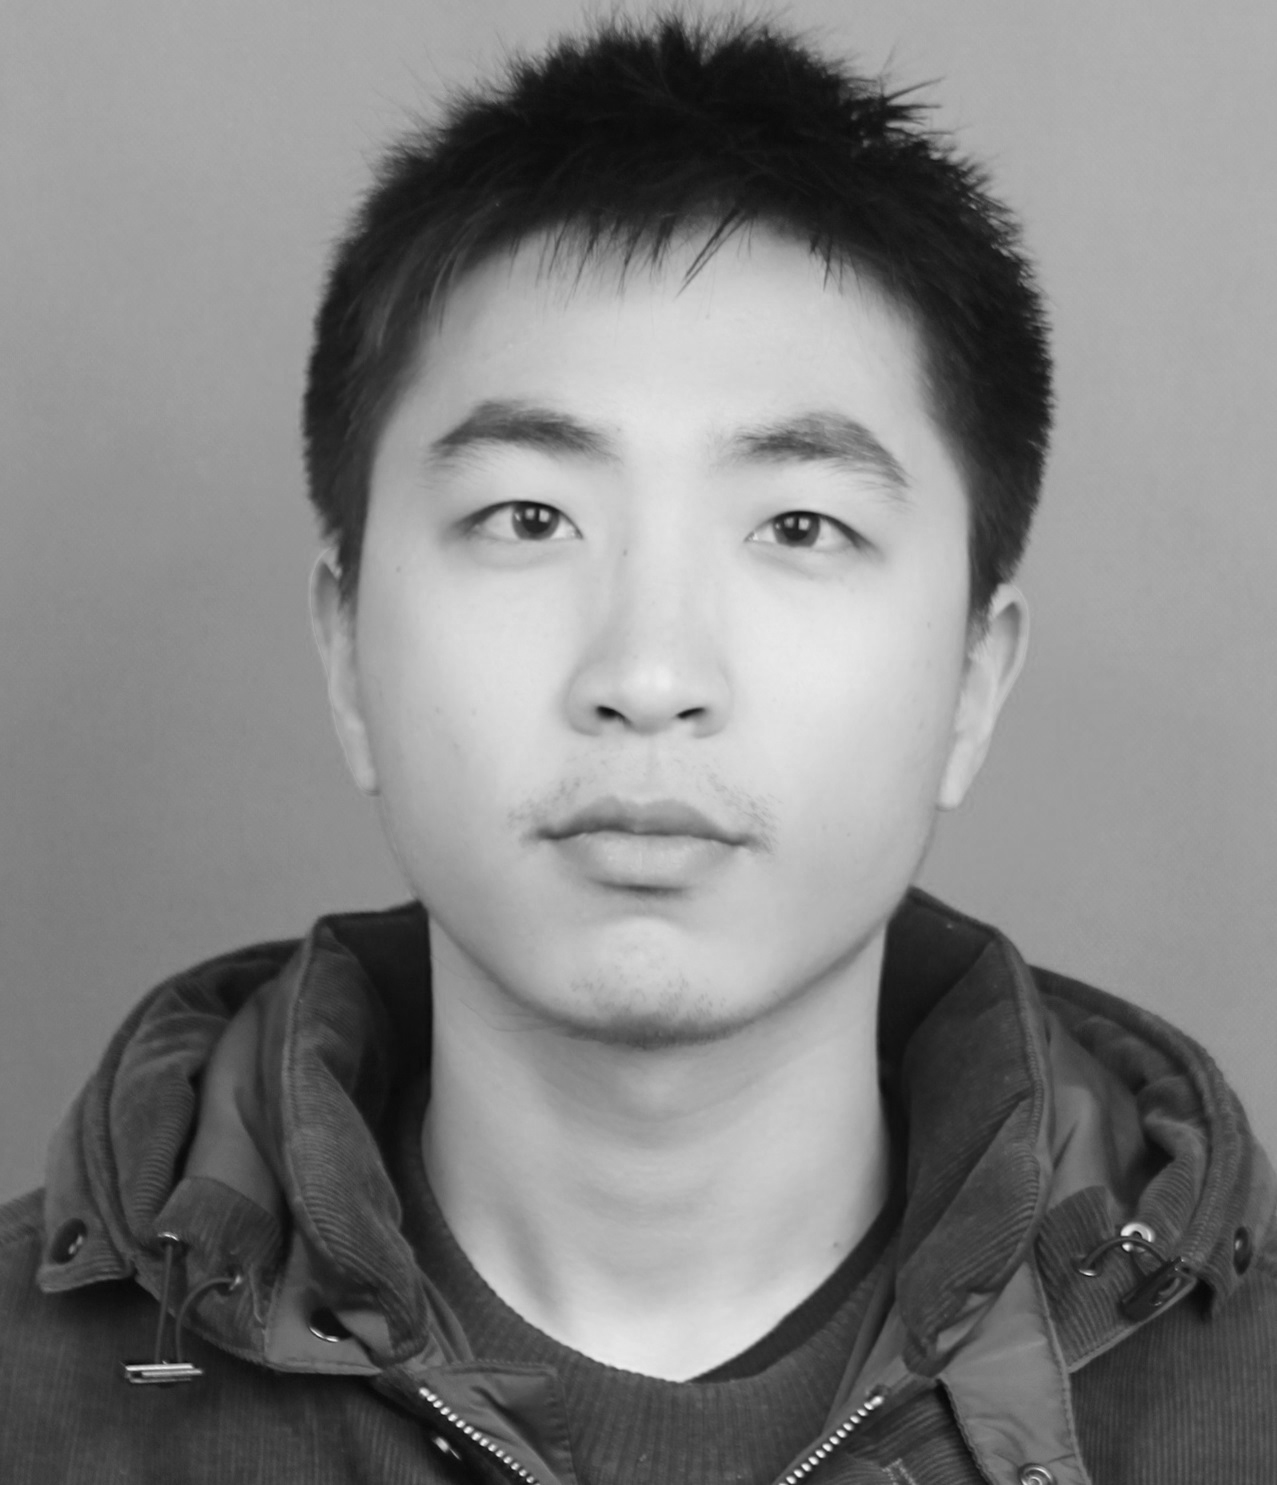
\includegraphics[width=1in,height=1.15in,clip,keepaspectratio]{niu}}]{Xintao Niu}
born in 1988, received his B.S degree from Nanjing University of Science and Technology. He is currently
working toward the PhD degree in the Department of Computer Science and Technology at
Nanjing University. His Research interest is software testing, especially on combinatorial testing and fault diagnosis. His work is supervised by Dr. Nie.
\end{IEEEbiography}

% if you will not have a photo at all:
\begin{IEEEbiography}[{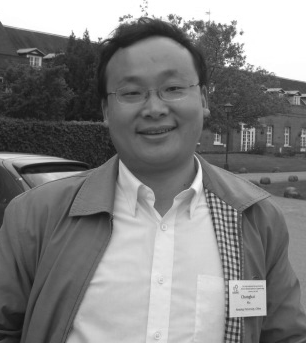
\includegraphics[width=1in,height=1.25in,clip,keepaspectratio]{nie}}]{Changhai Nie}
A Professor of Software Engineering in National Key Laboratory for Novel Software Technology and Department of Computer Science and Technology at Nanjing University. His research interest is software testing and search base software engineering, especially in combinatorial testing, search based software testing, software testing methods comparison and combination and et al.
\end{IEEEbiography}

\begin{IEEEbiography}[{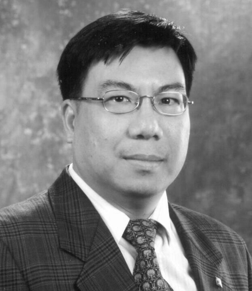
\includegraphics[width=1in,height=1.25in,clip,keepaspectratio]{hare}}]{Hareton Leung}
received the PhD degree in computer science from University of Alberta. He is an associate professor and the director at the Laboratory for Software Development and Management in the Department of Computing, the Hong Kong Polytechnic University. He currently serves on the editorial board of Software Quality Journal and Journal of the Association for Software Testing. His research interests include software testing, software maintenance, quality and process improvement, and software metrics
\end{IEEEbiography}

\begin{IEEEbiography}[{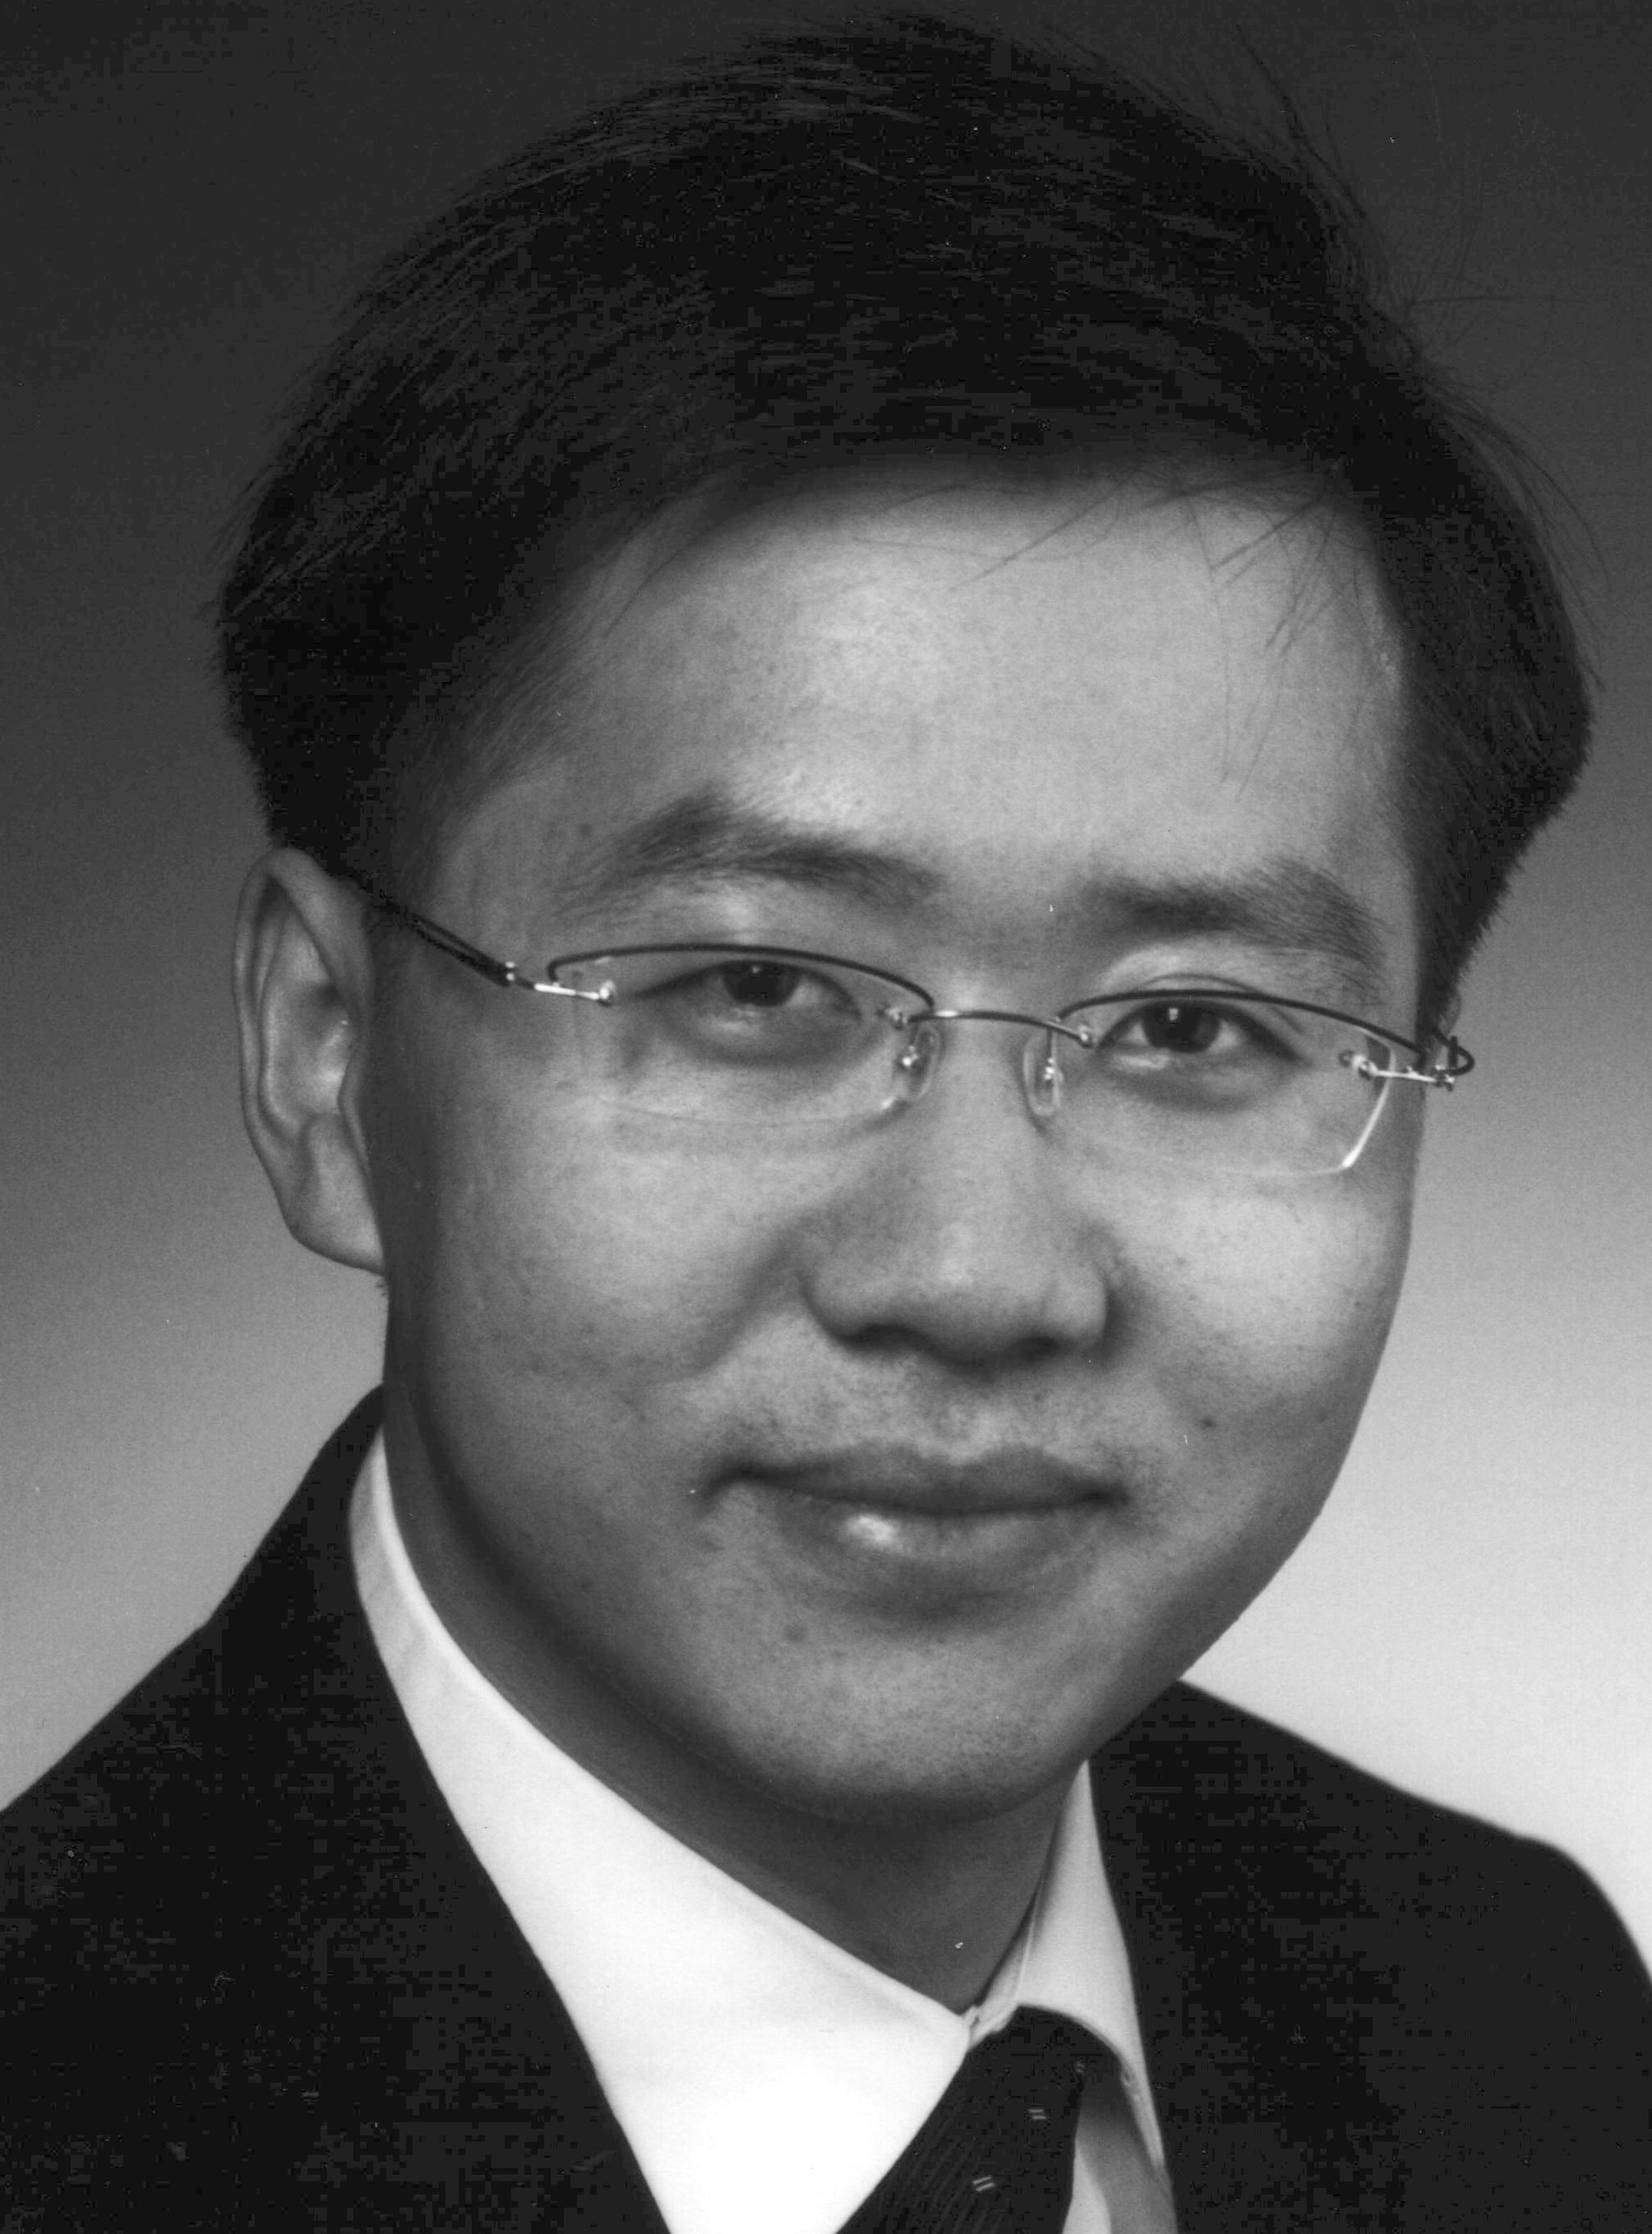
\includegraphics[width=1in,height=1.25in,clip,keepaspectratio]{lei}}]{Jeff Y. Lei}
is a full professor in Department of Computer Science and Engineering at the University of Texas, Arlington. He received his Bachelor's degree from Wuhan University (Special Class for Gifted Young), his Master's degree from Institute of Software, Chinese Academy of Sciences, and his PhD degree from North Carolina State University. He was a Member of Technical Staff in Fujitsu Network Communications, Inc. for about three years. His research is in the area of automated software analysis, testing and verification, with a special interest in software security assurance at the implementation level.
\end{IEEEbiography}

\begin{IEEEbiography}[{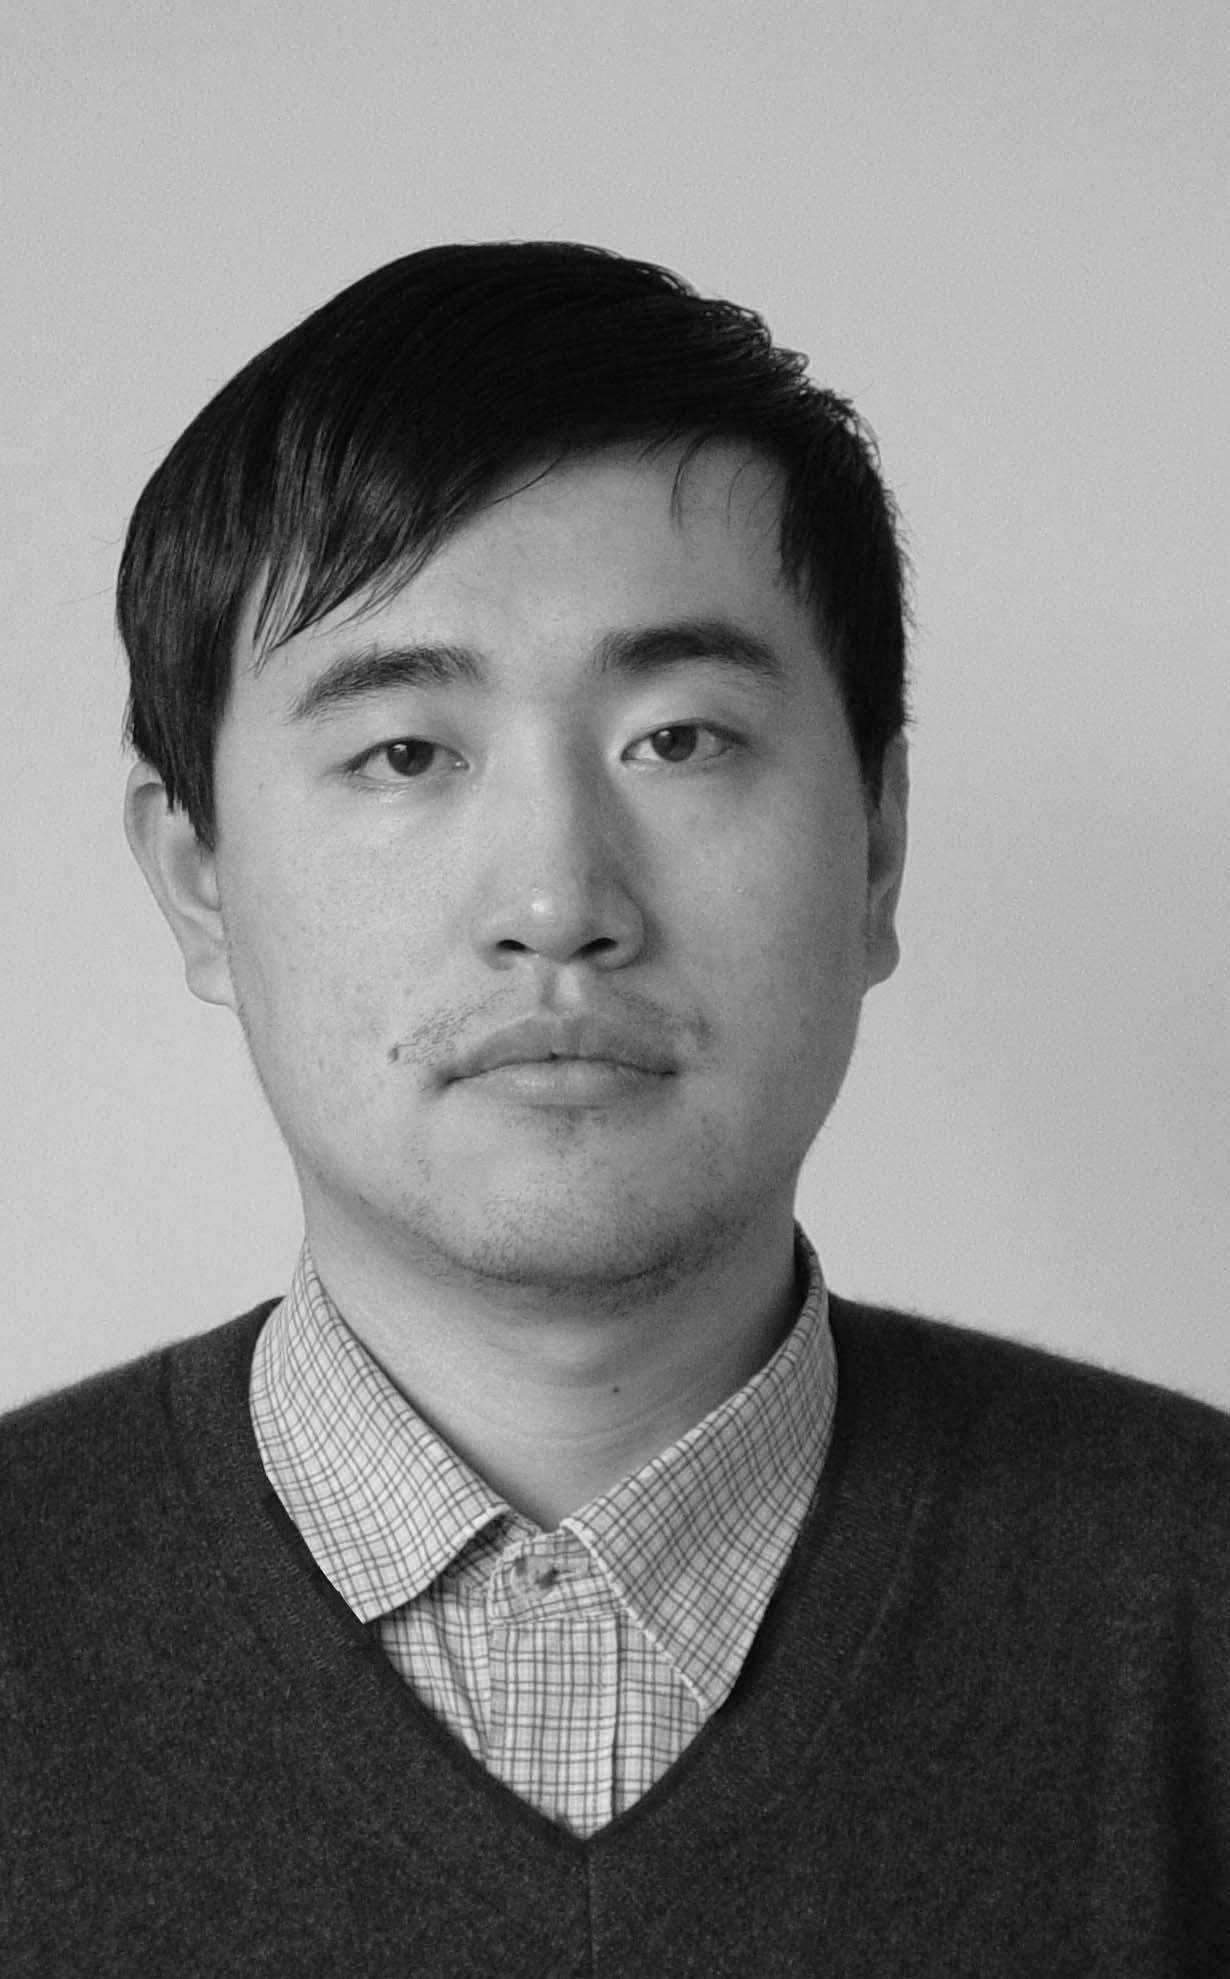
\includegraphics[width=1in,height=1.45in,clip,keepaspectratio]{xy}}]{Xiaoyin Wang}
born in Harbin, Heilongjiang Province, China in 1984. From September 2006 to January 2012, he was a Ph.D. candidate in the Software Engineering Institute (SEI) of Peking Univerisity. His advisor is Prof. Hong Mei, and he also did research under the supervision of Prof. Lu Zhang and Prof. Tao Xie. From Oct 2008 to Sept 2009, he visited Singapore Management University as a research fellow, where he worked with Prof. David Lo. In Jan. 2012, he began to work with Prof. Dawn Song, as a PostDoc in UC Berkeley. In August 2013, he joined the computer science department of University of Texas at San Antonio.
\end{IEEEbiography}

\begin{IEEEbiography}[{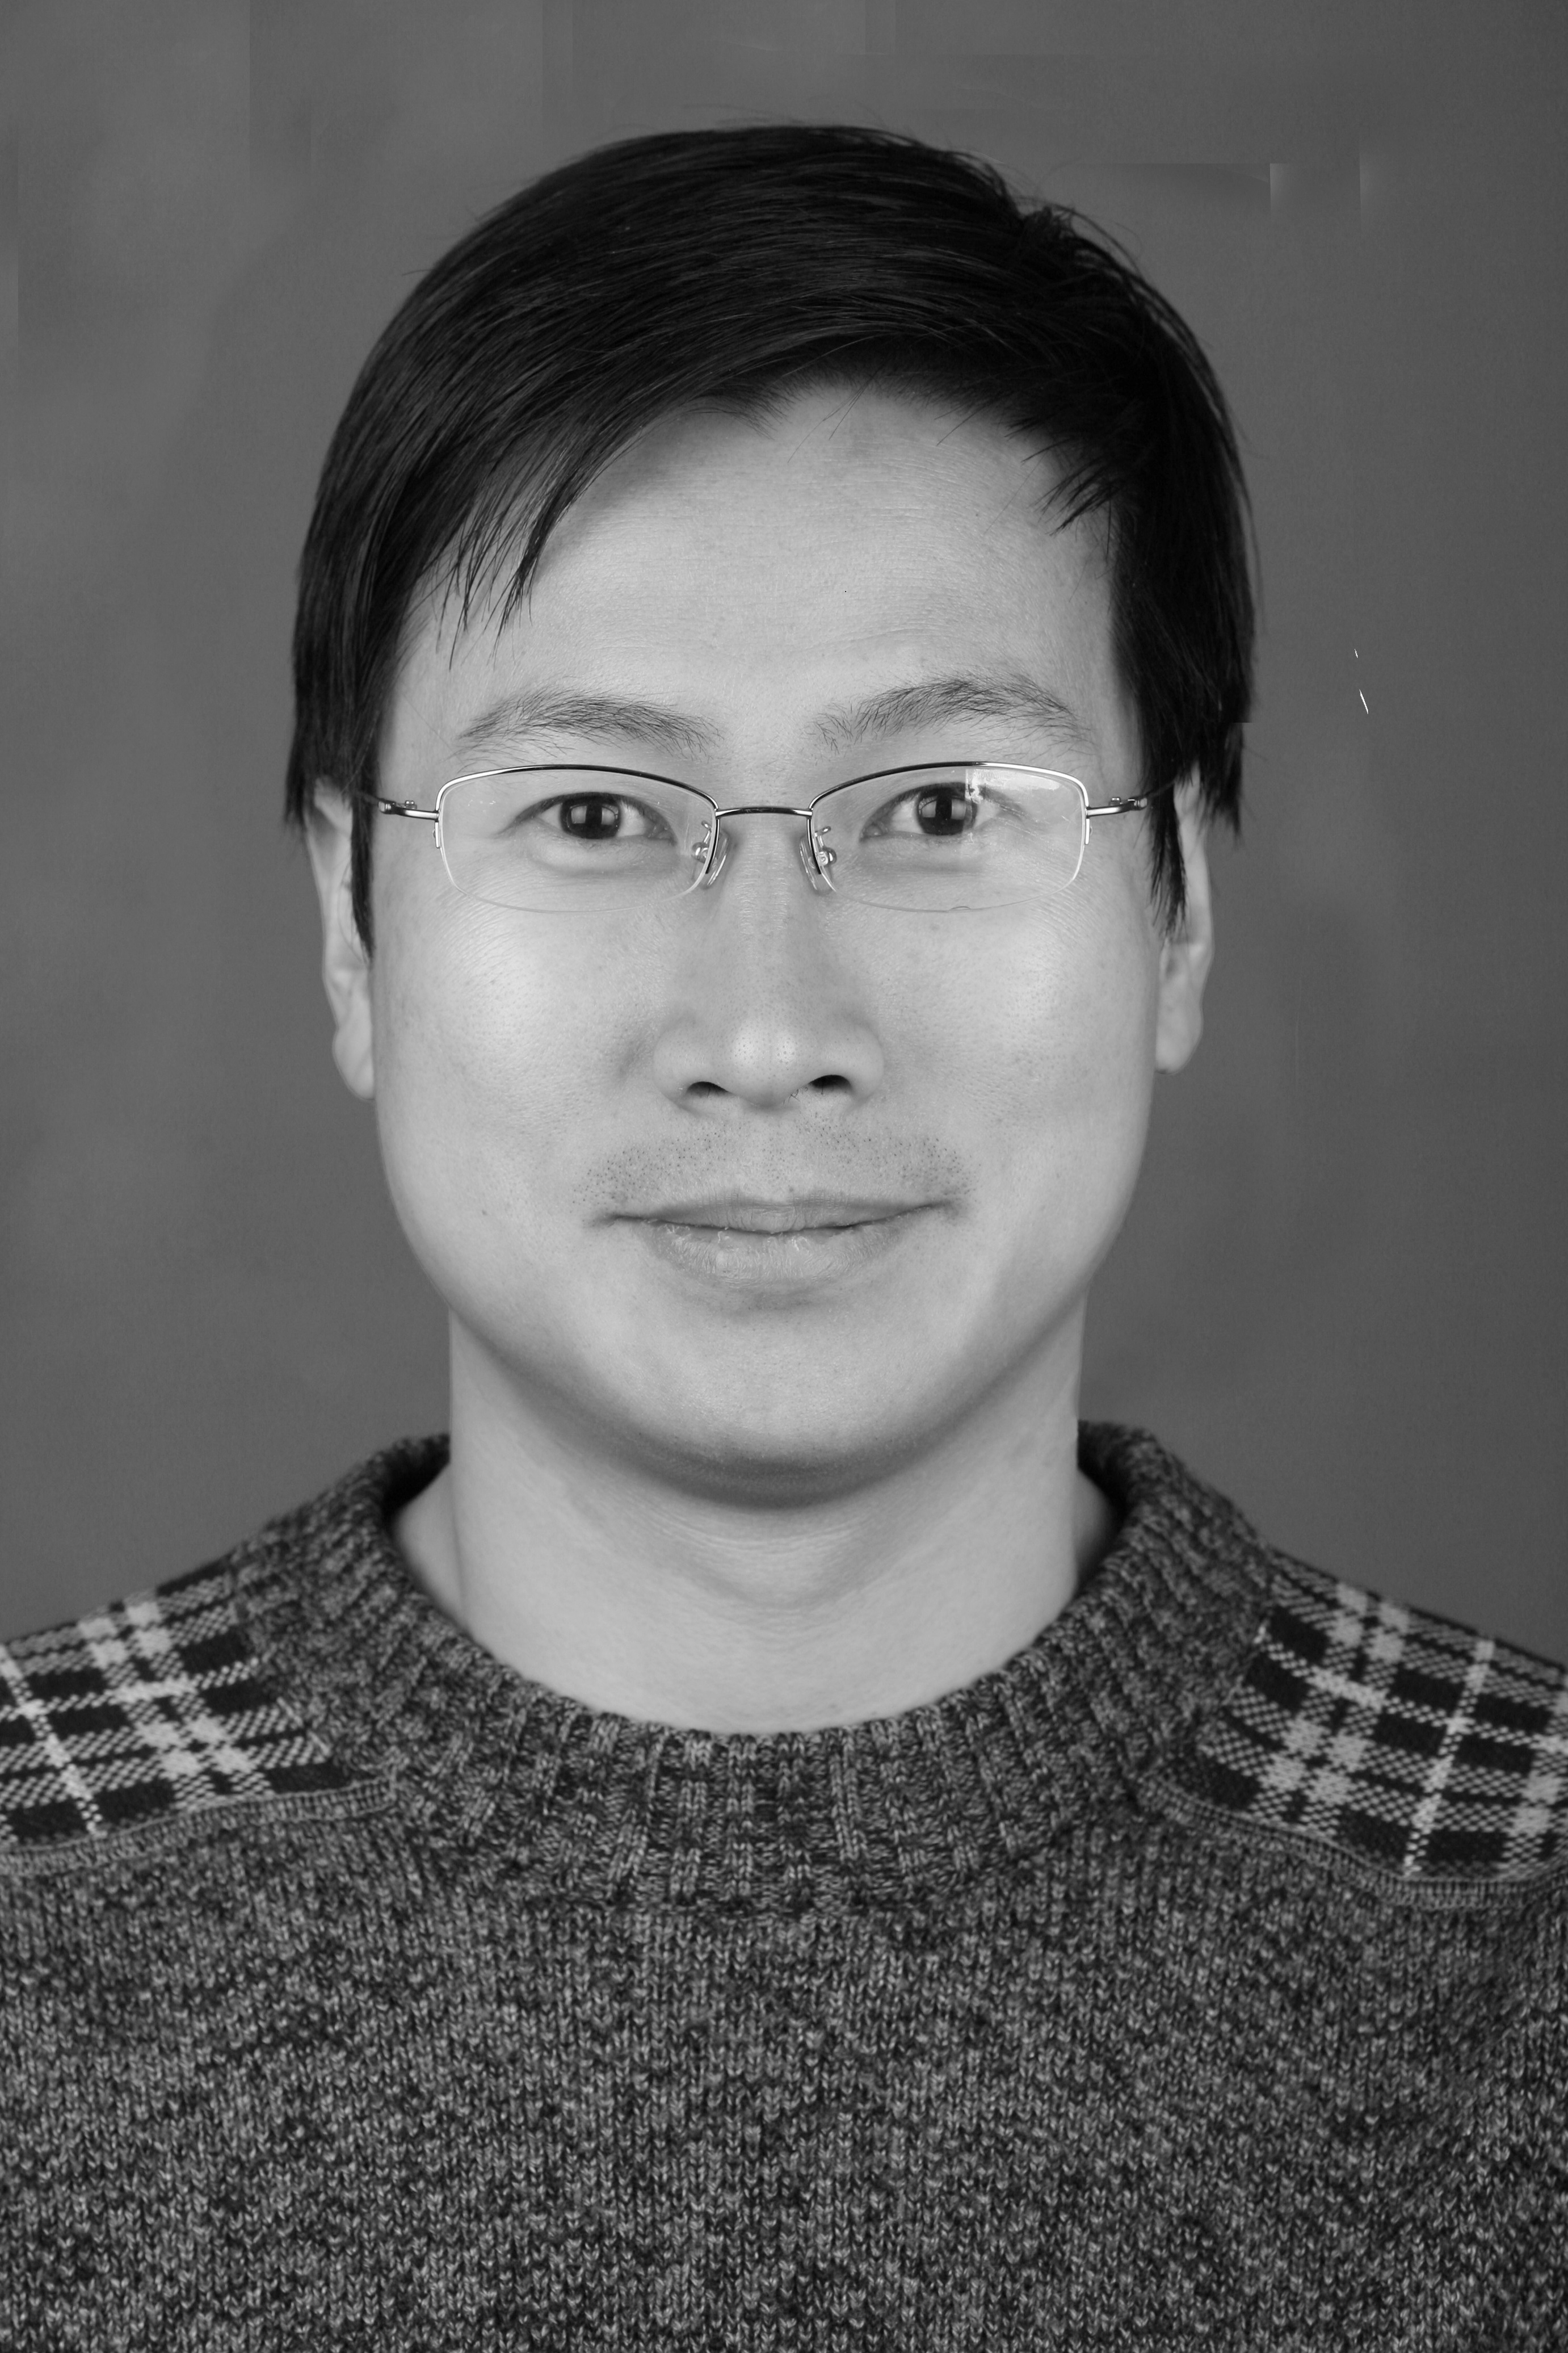
\includegraphics[width=1in,height=1.45in,clip,keepaspectratio]{xujiaxi}}]{Jiaxi Xu}
 born in 1972, Senior Engineer in School of Information Engineering of Nanjing Xiaozhuang University. His research interest is software testing, especially embedded software testing and open source software testing.
\end{IEEEbiography}

\begin{IEEEbiography}[{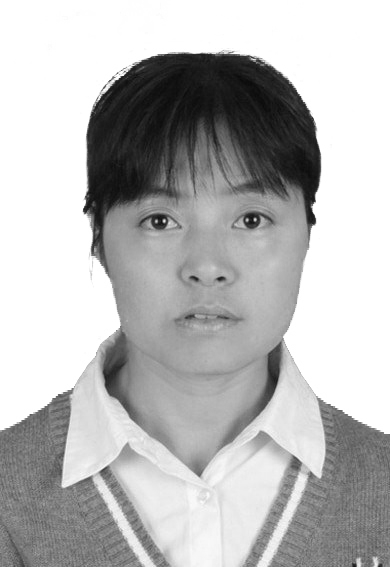
\includegraphics[width=1in,height=1.25in,clip,keepaspectratio]{wangyan}}]{Yan Wang}
received the MS degree in Control Theory and Control Engineering from University of Electronic Science and Technology of China. She is currently a lecturer in the School of Information Engineering at Nanjing Xiaozhuang University. Her research interests include development and testing of embedded software, and combinatorial interaction testing.
\end{IEEEbiography}

% You can push biographies down or up by placing
% a \vfill before or after them. The appropriate
% use of \vfill depends on what kind of text is
% on the last page and whether or not the columns
% are being equalized.

%\vfill

% Can be used to pull up biographies so that the bottom of the last one
% is flush with the other column.
%\enlargethispage{-5in}



% that's all folks
\end{document}


